\documentclass[floatsintext,doc]{apa6}
\usepackage{lmodern}
\usepackage{amssymb,amsmath}
\usepackage{ifxetex,ifluatex}
\usepackage{tikz}
\usetikzlibrary{bayesnet}

\usepackage{fixltx2e} % provides \textsubscript
\ifnum 0\ifxetex 1\fi\ifluatex 1\fi=0 % if pdftex
  \usepackage[T1]{fontenc}
  \usepackage[utf8]{inputenc}
\else % if luatex or xelatex
  \ifxetex
    \usepackage{mathspec}
  \else
    \usepackage{fontspec}
  \fi
  \defaultfontfeatures{Ligatures=TeX,Scale=MatchLowercase}
\fi
% use upquote if available, for straight quotes in verbatim environments
\IfFileExists{upquote.sty}{\usepackage{upquote}}{}
% use microtype if available
\IfFileExists{microtype.sty}{%
\usepackage{microtype}
\UseMicrotypeSet[protrusion]{basicmath} % disable protrusion for tt fonts
}{}
\usepackage{hyperref}
\hypersetup{unicode=true,
            pdftitle={Learning from generic language},
            pdfauthor={Michael Henry Tessler~\& Noah D. Goodman},
            pdfkeywords={keywords},
            pdfborder={0 0 0},
            breaklinks=true}
\urlstyle{same}  % don't use monospace font for urls
\usepackage{graphicx,grffile}
\usepackage{apacite}
\makeatletter
\def\maxwidth{\ifdim\Gin@nat@width>\linewidth\linewidth\else\Gin@nat@width\fi}
\def\maxheight{\ifdim\Gin@nat@height>\textheight\textheight\else\Gin@nat@height\fi}
\makeatother
% Scale images if necessary, so that they will not overflow the page
% margins by default, and it is still possible to overwrite the defaults
% using explicit options in \includegraphics[width, height, ...]{}
\setkeys{Gin}{width=\maxwidth,height=\maxheight,keepaspectratio}
\IfFileExists{parskip.sty}{%
\usepackage{parskip}
}{% else
\setlength{\parindent}{0pt}
\setlength{\parskip}{6pt plus 2pt minus 1pt}
}
\setlength{\emergencystretch}{3em}  % prevent overfull lines
\providecommand{\tightlist}{%
  \setlength{\itemsep}{0pt}\setlength{\parskip}{0pt}}
\setcounter{secnumdepth}{0}
% Redefines (sub)paragraphs to behave more like sections
\ifx\paragraph\undefined\else
\let\oldparagraph\paragraph
\renewcommand{\paragraph}[1]{\oldparagraph{#1}\mbox{}}
\fi
\ifx\subparagraph\undefined\else
\let\oldsubparagraph\subparagraph
\renewcommand{\subparagraph}[1]{\oldsubparagraph{#1}\mbox{}}
\fi

%%% Use protect on footnotes to avoid problems with footnotes in titles
\let\rmarkdownfootnote\footnote%
\def\footnote{\protect\rmarkdownfootnote}



% these packages are needed to insert results 
% obtained from R into the LaTeX document
\usepackage{pgfplotstable}
\usepackage{csvsimple}
\usepackage{siunitx}

% set the name of the folder in which the CSV files with 
% information from R is stored
\newcommand{\datafoldername}{csv_to_tex}

% the following code defines the convenience functions
% as described in the main text below

% rlgetvalue returns whatever is the in cell of the CSV file
% be it string or number; it does not format anything
\newcommand{\rlgetvalue}[4]{\csvreader[filter strcmp={\mykey}{#3},
             late after line = {{,}\ }, late after last line = {{}}]
            {\datafoldername/#1}{#2=\mykey,#4=\myvalue}{\myvalue}}

% rlgetvariable is a shortcut for a specific CSV file (myvars.csv) in which
% individual variables that do not belong to a larger chunk can be stored
\newcommand{\rlgetvariable}[1]{\csvreader[]{\datafoldername/myvars.csv}{#1=\myvar}{\myvar}\xspace}

% rlnum format a decimal number
\newcommand{\rlnum}[2]{\num[output-decimal-marker={.},
                             exponent-product = \cdot,
                             round-mode=places,
                             round-precision=#2,
                             group-digits=false]{#1}}

\newcommand{\rlnumsci}[2]{\num[output-decimal-marker={.},
                          scientific-notation = true,
                             exponent-product = \cdot,
                             round-mode=places,
                             round-precision=#2,
                             group-digits=false]{#1}}

\newcommand{\rlgetnum}[5]{\csvreader[filter strcmp={\mykey}{#3},
             late after line = {{,}\ }, late after last line = {{}}]
            {\datafoldername/#1}{#2=\mykey,#4=\myvalue}{\rlnum{\myvalue}{#5}}}

\newcommand{\rlgetnumsci}[5]{\csvreader[filter strcmp={\mykey}{#3},
             late after line = {{,}\ }, late after last line = {{}}]
            {\datafoldername/#1}{#2=\mykey,#4=\myvalue}{\rlnumsci{\myvalue}{#5}}}

\newcommand{\brmresults}[2]{\(\beta = \rlgetnum{#1}{key}{#2}{mean}{3}\) (\rlgetnum{#1}{key}{#2}{l95}{3}, \rlgetnum{#1}{key}{#2}{u95}{3})}
\newcommand{\brmresultsp}[2]{\(\beta = \rlgetnum{#1}{key}{#2}{mean}{3}\) [\rlgetnum{#1}{key}{#2}{l95}{3}, \rlgetnum{#1}{key}{#2}{u95}{3}]}
\newcommand{\effsize}[2]{\(d = \rlgetnum{#1}{key}{#2}{mean}{2}\) [\rlgetnum{#1}{key}{#2}{l95}{2}, \rlgetnum{#1}{key}{#2}{u95}{2}]}





  \title{Learning from Generic Language}
    \author{Michael Henry Tessler\textsuperscript{1}\textsuperscript{,2}~\& Noah D. Goodman\textsuperscript{1}}
    \date{}
  
\shorttitle{Learning from generic language}
\affiliation{
\vspace{0.5cm}
\textsuperscript{1} Department of Psychology, Stanford University \\
\textsuperscript{2} Department of Brain and Cognitive Sciences, Massachusetts Institute of Technology}
\keywords{generics; learning; pragmatics; semantics; Bayesian modeling \newline\indent Word count: 13699}
\usepackage{csquotes}
\usepackage{upgreek}
\captionsetup{font=singlespacing,justification=justified}

\usepackage{longtable}
\usepackage{lscape}
\usepackage{multirow}
\usepackage{tabularx}
\usepackage[flushleft]{threeparttable}
\usepackage{threeparttablex}

\newenvironment{lltable}{\begin{landscape}\begin{center}\begin{ThreePartTable}}{\end{ThreePartTable}\end{center}\end{landscape}}

\makeatletter
\newcommand\LastLTentrywidth{1em}
\newlength\longtablewidth
\setlength{\longtablewidth}{1in}
\newcommand{\getlongtablewidth}{\begingroup \ifcsname LT@\roman{LT@tables}\endcsname \global\longtablewidth=0pt \renewcommand{\LT@entry}[2]{\global\advance\longtablewidth by ##2\relax\gdef\LastLTentrywidth{##2}}\@nameuse{LT@\roman{LT@tables}} \fi \endgroup}
\usepackage{tabularx}
\usepackage{multicol}
\usepackage{wrapfig}
\usepackage{caption}
\usepackage{booktabs}
\usepackage{amsmath}
\usepackage{graphicx}
\usepackage{subcaption}
\usepackage{longtable}
\usepackage{array}
\usepackage{multirow}
\usepackage{xcolor}
\usepackage{bbm}

\newcommand{\denote}[1]{\mbox{ $[\![ #1 ]\!]$}}
\newcommand*\diff{\mathop{}\!\mathrm{d}}
\definecolor{Red}{RGB}{255,0,0}
\definecolor{Green}{RGB}{10,200,100}
\definecolor{Blue}{RGB}{10,100,200}

\newcommand{\mht}[1]{{\textcolor{Blue}{[mht: #1]}}}
\newcommand{\ndg}[1]{{\textcolor{Green}{[ndg: #1]}}}
\newcommand{\red}[1]{{\textcolor{Red}{#1}}}

\authornote{Corresponding author: Michael Henry Tessler, 450 Serra Mall, Building 420, Department of Psychology, Room 316, Stanford University, Stanford, CA 94305, USA. E-mail: \href{mailto:tessler@mit.edu}{\nolinkurl{tessler@mit.edu}} Present address: Department of Brain and Cognitive Sciences, Building 46, Room 3027,	Massachusetts Institute of Technology, 77 Massachusetts Avenue, Cambridge, MA 02139-4307, USA}

\abstract{
Generic language (e.g., \emph{Birds have hollow bones}) conveys generalizations about categories and is a fundamental and ubiquitous mechanism of learning about the world. 
How exactly this learning occurs, however, is unclear: Generics exhibit so much flexibility in how they are interpretated that a quantitative theory of how generics update beliefs has not only  not been developed or tested, but is often explicitly dismissed.
%with respect to what makes them true or false  % been developed and tested.
%Understanding generics, however, involves an extreme dependence on context that has made 
%Articulating precisely how generic language updates beliefs, however, is beyond the reach of any extant theory of generics.
Here, we explore a hypothesis introduced by Tessler and Goodman (2019) that generics update beliefs via an uncertain threshold like a vague quantifier: A category--property generic (\emph{Ks F}) means that the property F is expected to be relatively widespread in the category K, where what counts as being relatively widespread is \emph{a priori} uncertain and resolved by consulting one's prior beliefs about the property. 
We compare this model to a family of alternatives with the same background knowledge but where generics have a fixed, precise meaning; in addition, we formalize a quantitative model of a strictly conceptual-based approach to generics, where generics are a direct connection to conceptual knowledge.
Across three experiments in which we both measure and manipulate prior beliefs, we find the uncertain meaning approach to generics to be the best explanation of participants' highly heterogeneous interpretations of novel generic statements. 
This result taken together with the result that the same model of generic meaning can explain the variability in  generic endorsements as shown by Tessler \& Goodman (2019) suggests that generics are an effective medium for faithful transmission of knowledge between interlocutors. 
This work adds to the growing enterprise of formal, quantitative studies of human understanding of generic language.
%manifests in a directly analogous manner in interpretations. %generics
% we both measure and manipulate prior beliefs. We find that prior beliefs are causally related to generic interpretations, as predicted, and that  are best modeled as a vague quantifier.
% Our results confirm previous arguments that simplistic statistical models of generics are untenable, while also providing a path forward for a rigorous quantitative study of generic language.
%proposed a model for a meaning of generics as a vague quantifier, which predicted truth judgments (or, endorsements) of generics with high quantitative accuracy. 
%Learning, however, operates via belief-updating and the question still remains about how generic language updates beliefs. 
%Here, we test the adequacy of this model to account for the belief-updating capacity of generic statements -- how novel generics are interpreted by listeners -- and compare it to other possible quantitative models of belief-updating from generics.
%Here, we formalize a simple hypothesis about the meaning of generics:  Borrowing the machinery of learning from observations, generics convey a single, minimal example to the listener. 
%We show this model is mathematically equivalent to a recent proposal by Tessler and Goodman (2019) for generics as a kind of vague quantifier. 
%We extend their model with a mechanism for pragmatic interpretation and test the models in their ability to account for the belief-updating resulting from generic statements---how novel generics are interpreted by listeners. 
%The vague quantifier model of generics predicts strong dependence of interpretation on prior beliefs about the prevalence of features. 
%We also show that the generics-as-minimal-example theory relates to traditional, quantificational views of generics in a straightforward way.
}

\begin{document}
\maketitle
%\newpage


\hypertarget{introduction}{%
\section{Introduction}\label{introduction}}

%\mht{might want to make the point somewhere in the intro, or model section, that it is hard to test quantitative models for generic interpretations because (a) interpretations are highly variable and (b) background knowledge is hard to partial out}

Much of what we learn about the world comes not from our own experience but by learning from others, often via language.
Language is a powerful medium through which to describe that which goes beyond what can be experienced, conveying abstractions and generalizations.
Generalizations about categories are often conveyed using generic language \cite<e.g., \emph{Birds have hollow bones}; \emph{Alligators grow to be 10-feet long};>{Carlson1977}, an important case of abstract knowledge transmitted through language \cite{Gelman2009}.
Generics are ubiquitous in everyday conversation and child-directed speech \cite{Gelman1998, Gelman2008, Gelman2004mono}, and learning from generics is thought to be central to conceptual development \cite{Cimpian2009:explanations, Gelman2004}.
Understanding how beliefs are updated from generic language is thus an important issue for cognitive science.

%\mht{THOUGHT: Is there a way to start with RSA, and then ask what is the literal contribution of a generic? TG19 give us one.... One way might be to take the Abelson intuition, and then reason through 

One of the most fundamental components of beliefs are the latent probabilities that we use to make predictions about the future \cite{Shepard1987}. 
For a standard category-based prediction problem, the relevant metric is the probability that an instance of a category $k$ has a feature $f$: $P(f \mid k)$, sometimes referred to as the \emph{prevalence} of the feature in the category.
%The most basic, theory-neutral dimension of belief-updating about categories and properties is the prevalence of a feature in a category, or :
A common intuition with generics is that they \enquote{{[}\ldots{}{]} appear to be commonly taken [\emph{interpreted}] in a rather strong sense, as though the qualifier \emph{always} had implicitly crept into their interpretation} \cite<p.~172,>{Abelson1966}; in other words, a common intuition is that generics mean \emph{all}, or a generic conveys that $P(f \mid k) =1$. 
Generics allow for exceptions, however (e.g., not all birds fly, yet \emph{Birds fly} is a true statement), and so the generic must allow for $P(f \mid k) < 1$. 
Some generics seem to convey prevalence levels substantially less than 100\%: \emph{Robins lay eggs} intuitively conveys that roughly 50\% (the female robins) lay eggs ($P(f \mid k) \approx 0.5$); \emph{Mosquitos carry malaria} conveys a low prevalence value (in true fact, $< 1\%$ of mosquitos carry malaria; $P(f \mid k) \approx 0.01$). 
Broadly consistent with these intuitions, prior research has found that adults typically rate the prevalence implied by a generic (e.g., \emph{Bears like to eat ants}) to be very high \cite<\emph{most bears like to eat ants};>{Gelman2002}, except when the features could be construed as being accidental, in which case prevalence is rated substantially lower (e.g., \emph{Xs have fungus-covered claws} $\rightarrow$ \emph{some Xs have fungus-covered claws}; \citeNP{Cimpian2010}; see also \citeNP{Khemlani2009, Khemlani2012} for evidence of similarly weak inferences from generics such as \emph{Lions eat people}).

%learning from generics about both familiar and novel animals (e.g., \emph{Bears like to eat ants}; \emph{Lorches have purple feathers}) rate the prevalence of the feature implied by the generic (e.g., the percentage of bears that like to eat ants) 
%Another common intuition, however, is that generics can convey weak generalizations.
% For example, \emph{Mosquitos carry malaria} seems to only convey that the prevalence is non-zero, an existential claim, as if the qualifier \emph{can} had implicitly crept in: \emph{mosquitos can carry malaria}.
% Consistent with this intuition, \citeA{Cimpian2010} (Expt.~3) found lower implied prevalence from generics about%Even more puzzling, generics can take on other interpretations --- distinct from \emph{all}, \emph{most}, or \emph{some} --- as in the case of \enquote{Ducks lay eggs}, where half of ducks (the females) lay eggs.

%TStipulated that a generic implies $P(f \mid k)$ is high cannot be the full story:
%Intuitively, such strong interpretations could arise through pragmatic reasoning \cite{Grice1975}: Why would a speaker assert a generic claim unless the property (e.g., eating ants) were sufficiently prevalent in the category?
%Generics exhibit extreme sensitivity to context, however, that has made it difficult to define quantitatively what should be learned from a generic.
%Intuitively, generics \enquote{{[}\ldots{}{]} appear to be commonly taken in a rather strong sense, as though the qualifier \emph{always} had implicitly crept into their interpretation} (p.~172; Abelson \& Kanouse, 1966), and indeed adults learning from generics about both familiar and novel animals (e.g., \enquote{Bears like to eat ants}; \enquote{Lorches have purple feathers}) rate the \emph{implied prevalence} of the feature (e.g., the percentage of bears that like to eat ants) as very high (\(\sim 85\%\); Gelman, Star, \& Flukes, 2002; Cimpian, Brandone, \& Gelman, 2010, Expt. 1).

%And how would a learner, hearing a novel generic, know how strongly to interpret it?

%If, in fact, \enquote{Mosquitos carry malaria} conveys something very weak, analogous to \emph{some mosquitos, under some circumstances, carry malaria}, then the knowledge conveyed by the generic could be similar to learning one mosquito, in one particular circumstance, was once observed carrying malaria; then, given that properties covary with kinds in systematic ways, a learner might reasonably infer that there is some larger (but unknown) subset of mosquitos in some larger (but unknown) class of situations that also carry malaria.

The fact that generic statements have such variable interpretations in terms of the property prevalence $P(f \mid k)$ has been taken by many in psychology to imply that there is no coherent, quantitative relationship between the meaning of generics and the prevalence of the feature \cite{Leslie2008, Cimpian2010, Khemlani2012, Prasada2013}. 
Instead, theory-building has proceeded with verbal accounts, appealing to notions of kindhood and conceptual structures, whose relation to quantitative data is often underspecified.
% so many diverse  that the predicated property is present in all, most, half, some, or few members of a category 
% different levels of prevalence of interpretations that are possible with generic sentences has been taken
%This conclusion does not follow, however, since these studies only show that a single
The fact that generics have variable interpretations, however, does not falsify the notion that there exists a systematic relationship between generics and prevalence.
Generics, like many other aspects of language, may exhibit a sensitivity to context  which  modulates how they get interpreted; such a context-sensitivity does not in and of itself rule out that generics update beliefs about prevalence in a consistent, predictable way (see \citeNP{kochari2020generics} for a related argument). 
% It is this project we concern ourselves with here.
% Developing and testing such a context-based, statistical account of generics is methodologically challenging, however: One must articulate a model of generics that describes precisely how context and the meaning of generics combine to produce an interpretation in the mind of a learner, and one must quantitatively validate such a model by measuring interpretations of generics and prior beliefs and relating the two via the model.

% Tessler \& Goodman did this very thing. 
% But they didn't test how this would work in interpretation. 
%They also didn't try to formalize what

\citeA{Tessler2019psychrev} proposed a quantitative account of generics that synthesized and unified this diverse swath of linguistic expressions. 
Under this model, the core meaning of a generic is a kind of vague quantifier (a la \emph{many} or \emph{a lot}) but one whose precise meaning is underspecified and must be inferred in context, which takes the form of shared, conceptually-based prior knowledge about categories and properties. 
% (a la \emph{some}, \emph{most}, \emph{all}) in the sense that its truth conditions are determined by a threshold function (e.g., \emph{some} means at least one,  \emph{most} means at least half); the generic is a special kind of quantifier, however, because the threshold for the generic is underspecified and must be inferred in context (i.e., the generic means: at least $\theta$, where $\theta$ is unknown).
%The threshold is resolved by a Bayesian listener reasoning about the probabilities of different levels of prevalence for a given feature; for example, carrying malaria is a property whose prevalence in a category is expected to be low because among other categories, the property exists in only a few members of a category when it is present at all (e.g., a few birds may have malaria, but it is implausible that all members of a category would be carrying malaria at any particular moment in time). 
The model was shown to explain truth judgments or endorsements (e.g., is the sentence \emph{Mosquitos carry malaria} true or false?) with a high-degree of quantitative accuracy, but it also provides a yet-untested substantive hypothesis about interpretations, or how beliefs should be updated from generic language. 
%These predictions have never been tested, however, and it is on interpretations that we focus on in this paper.
%It is these
% belief-updating or interpretations has not been tested and is important for understanding learning from generic language.


%even when a member of a certain category is \emph{carrying malaria}, it is relatively unlikely that most or all other members of the category are also \emph{carrying malaria}.


% over subjective, predictive probabilities that result from richly structured prior knowledge about categories and properties. 
%The model uses simple Bayesian reasoning to determine which threshold is likely to be true, given  prior knowledge of the property. 
%Yet, prior knowledge alone may not be the sole contributor to generic interpretation. 
%In particular, communicative, pragmatic pressures could enrich the literal meaning of the generic in fundamental ways \cite{declerck1986manifold}.
%We thus extend this original model using the tools developed in the Rational Speech Act framework \cite{Frank2012, Goodman2016, problang}, a class of probabilistic models of pragmatic communication, to better understand how pragmatic reasoning could enrich the literal interpretation of a generic.

%We draw a different conclusion from this evidence.



%Rather than 
%What sort of meaning could account for the panoply of interpretations that come with generic sentences?

%In addition, pragmatic communicative pressures 
%
%such strong interpretations could arise through pragmatic reasoning \cite{Grice1975}: Why would a speaker assert a generic claim unless the property (e.g., eating ants) were sufficiently prevalent in the category?
%
%
%\mht{mention that we measure quantitative data for priors and interpretation, which supports the full pragmatic generic model}. 

%Furthermore, we test this pragmatic generic interpretation model in its ability to model the belief-updating aspect of generics; the earlier work tested 
%Testing interpretation is crucial given the role of generic language in learning. 

%Updating one's beliefs by observing examples is a very basic cognitive ability, shared with other animals. 
%It is thus a reasonable starting point to imagine that language has coopted this belief-updating mechanism, and that the meaning of a generic is equivalent to ``imagine you have observed an example.''
%That is, hearing \enquote{Mosquitos carry malaria} is interpreted as the knowledge that one mosquito, in one particular circumstance, was once observed carrying malaria; belief updating from this one ``observation'' would affect our beliefs about other mosquitos, given that properties tend to have some consistency within kinds.
%If a generic conveys a single, positive example, the example would be a \emph{minimal example} in the sense that it would exhibit only the feature being described by the predicate in the generic sentence, while other features remain unknown.
%Bayesian belief-updating is a standard way to formalize this reasoning, that has been found to match complex patterns of human learning (Tenenbaum, Kemp, Griffiths, \& Goodman, 2011).
%%ne could formalize the meaning of a generic statement as equivalent to Bayesian belief-updating of structured prior knowledge (Tenenbaum, Kemp, Griffiths, \& Goodman, 2011) after observing a single positive example of the category with a property.
%Later we show that construing generic interpretation as Bayesian belief-updating from a single minimal example is mathematically identical to a recent model by Tessler and Goodman (2019) that treats a generic as a vague quantifier.

%The hypothesis that the core meaning of a generic is a vague quantifier provides only the literal contribution of the utterance, but language is never heard in a vacuum, sampled from some random process. 
%Instead, language is understood in a social context (Grice, 1975): Why did the speaker bother to tell me this?
%\mht{mention the kind of ``implicit'' pragmatics we have in mind? Levinson (1996?): pragmatics pervades even logical reasoning?}
%%Such pragmatic reasoning is pervasive, and need to
%We show in this paper that communicative or pragmatic reasoning, formalize in a Rational Speech Act model (Frank \& Goodman, 2012; Goodman \& Frank, 2016; Scontras, Tessler, \& Franke, 2018), can give rise to richer interpretations of generics than the literal content would necessarily convey. 
%In this paper, we test a literal model of generic interpretation against a pragmatic model, which we 


%The information conveyed by a generic may still be more than that encoded by just a single positive example.
%One plausible source for deriving stronger interpretations is social, communicative reasoning That is, pragmatic enrichment of the literal content of generics could manifest as a stronger implied prevalence than just that implied by a single example.
%The idea that generics convey a communicatively relevant example to the listener is consistent with a view of generics as a fundamentally pedagogical---and not necessarily linguistic---phenomenon (Csibra \& Shamsudheen, 2015).

In addition to these theoretical questions, basic empirical questions about context-sensitive generic interpretation remain.
Previous experimental work on interpretations of generic statements have revealed categorical distinctions (e.g., generics about properties of accidental or disease states are interpreted less strongly than generics about biological properties; \citeNP{Cimpian2010}), but the extent of the gradience in generic interpretations has never been examined or quantified in an experiment. 
Furthermore, though intuitively generics can have weak interpretations (e.g., implying that only a minority of the category have the property), the implied prevalence from the weakest of generics in these previous studies was still quite high (e.g., around 70\% in \citeNP{Cimpian2010} Expt. 3), leaving open the question of how weak generic interpretations can be.\footnote{Similarly, inferences that members of a category have a property (e.g., \enquote{Leo is a lion. Thus, Leo eats people.}) can be quite weak, though still the extant empirical evidence suggests participants still think that the inference is more likely than not \cite{Khemlani2012}.\footnote{In this study of \citeA{Khemlani2012}, the measurement was actually a confidence rating on -3 to +3 scale. All reported mean confidence ratings were greater than the midpoint of the scale.}
}
Our formal modeling predicts gradience in interpretations and that such very weak interpretations can occur when prior knowledge indicates that the property in question is rare within kinds (e.g., the property only manifests under certain circumstances).

%  bonafide weak interpretations (e.g., implied prevalence \(<50\%\)) can result when learning from novel generics.
%
%Though the intuitive implied prevalence of \emph{Mosquitos carry malaria} is very low (i.e., very few mosquitos carry malaria), the sentence is just one example and the empirical data supporting a more general conclusion about the existence of weak generics is mixed.
%In \cite{Cimpian2010} (Expt. 3), the mean implied prevalence from weak generics was \(70\%\) (i.e., after hearing a generic, the predicated property was expected to be present in 70\% of the category), significantly lower than that observed for generics about biological properties, but still conveying that a majority of the category have the property.
%Further, the gradience in generic interpretations has never been examined or quantified in an experiment. 

This paper is organized as follows.
In the first section, we describe the model of generic meaning proposed by \citeA{Tessler2019psychrev} and show how it predicts prevalence interpretations from a generic statement.
We additionally describe alternative models that predict prevalence interpretations from different assumptions about the meaning of a generic; as well, we formalize a model that predicts prevalence by assuming generics serve as a kind of direct conduit to conceptual knowledge.
We compare these formal hypotheses in their abilities to predict and provide a parsimonious explanation for generic interpretation data from three experiments, in which we both measure prior beliefs and generic interpretations.
%and incorporate it into the Rational Speech Act modeling framework \cite{Frank2012, Goodman2016}.
%We compare literal and pragmatic versions of the model against additional control models that use the same prior knowledge but which update their beliefs via different semantic mechanisms: fixed-thresholds analogous to the semantics of quantifiers like \emph{some} and \emph{most}.
In Experiment 1, we test the models on a diverse stimulus set designed to elicit high by-item variability.
In Experiment 2, we examine the models in their capacity to explain data from a replication of \citeA{Cimpian2010} (\emph{Implied Prevalence} task).
% that biological and accidental properties receive differential interpretations and find substantial variability in implied prevalence by-item; the items that exhibit the most variability, however, have a potential confound which leads us to design our main experiments.
%use these data to test our literal and pragmatic models of generic interpretation against each other and against control models.
In Experiment 3, we test whether prior beliefs about prevalence are causally related to the interpretation of a novel generic by experimentally manipulating prior beliefs.
Together, these results provide strong quantitative evidence that generics update beliefs about prevalence in a coherent, consistent way as predicted by the model of \citeA{Tessler2019psychrev}.


%We conclude by discussing the broader context of these results and their importance for our understanding of learning and development.



%\begin{enumerate}
%\item connect ``context'', ``prior beliefs about context'' and ``prior beliefs about prevalence of features''
%\item introduce uncertain threshold account and fixed-threshold alternatives
%\item fixed-threshold alternatives are a sort of validation of the cimpian, leslie intuition... no fixed-threshold model is a good model
%\item uncertain threshold is a systematic relationship between prevalence and generics (just like gradable adjectives)
%\end{enumerate}



%\begin{figure}
%\centering
%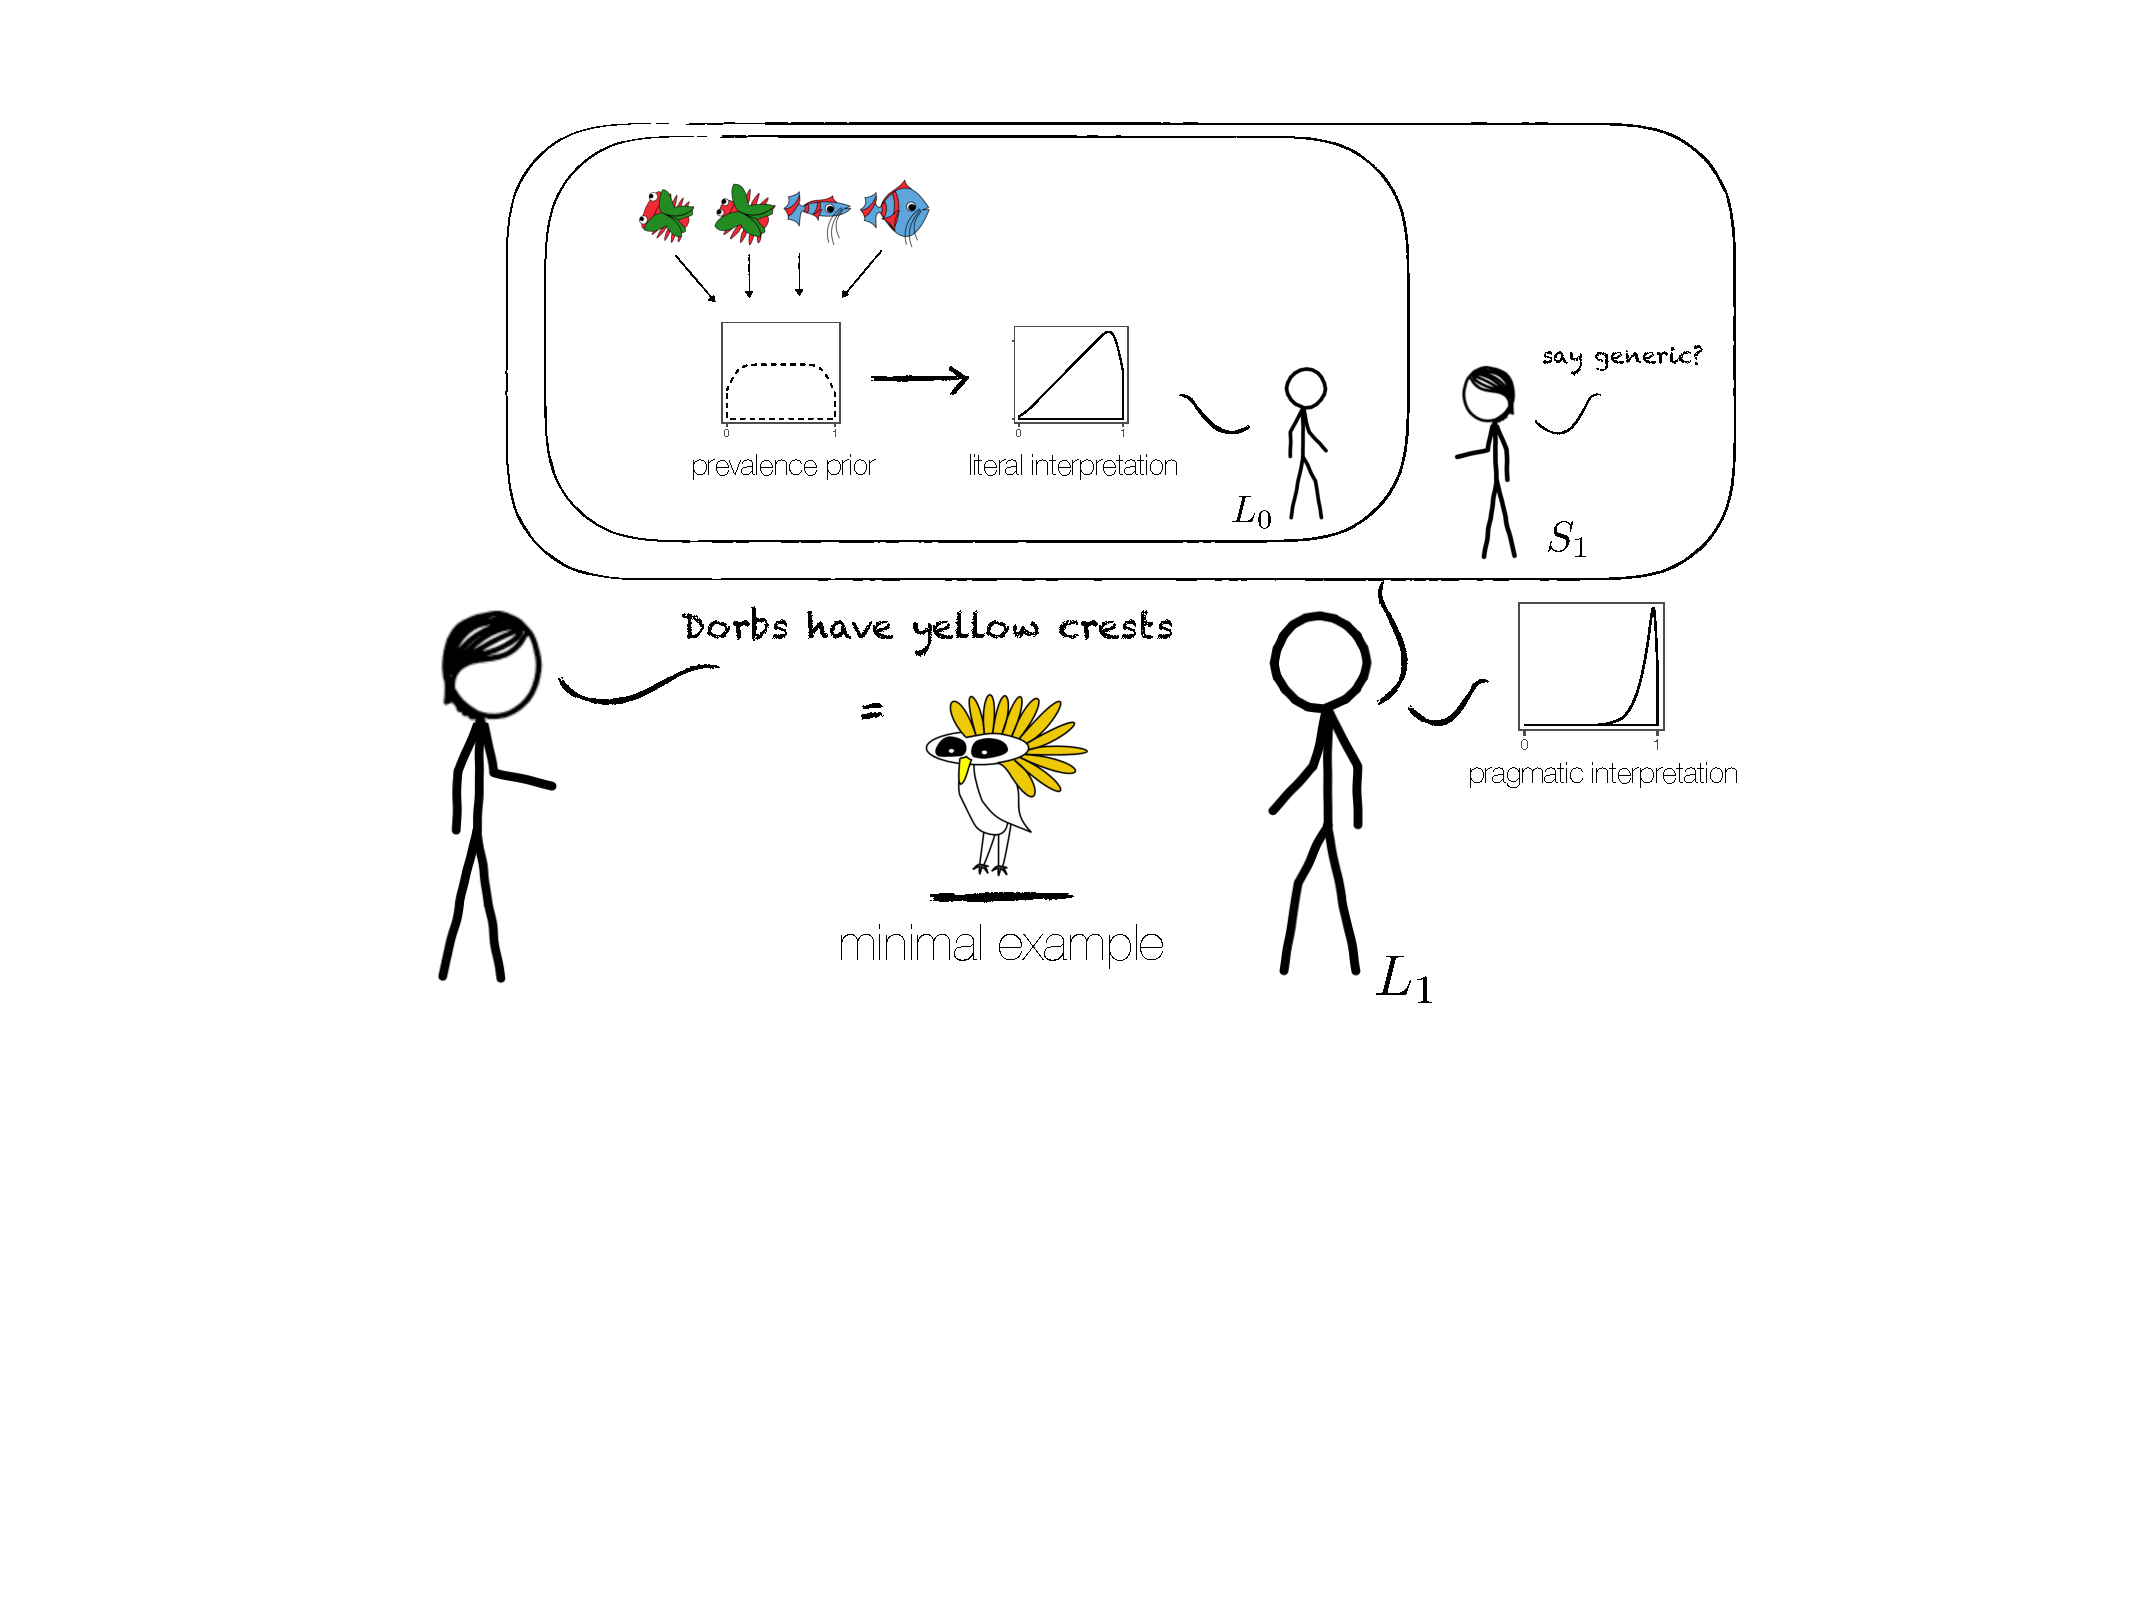
\includegraphics{figs/cartoon3.pdf}
%\caption{\label{fig:cartoon}Cartoon of the pragmatic generic interpretation model. The literal contribution of a generic (e.g., \enquote{Dorbs have yellow crests}) is a threshold function where the listener is uncertain about the threshold. 
%%\ndg{add a creature within the L0 bubble that has no colors except the yellow crest (ie make minimal), and label it "dorb". also maybe replace the arrows from agents to creatures with an eye?} 
%A pragmatic listener (\(L_1\)) interprets the utterance as a communicative act coming from a speaker (\(S_1\)) that decides to produce a generic in order to convey prevalence information to a naive listener (\(L_0\)). 
%The literal listener interprets the utterance (\emph{literal interpretation}) by drawing on their prior knowledge about other categories and properties (\emph{prevalence prior}).}
%%\mht{make this into something more like }
%\end{figure}

\hypertarget{computational-model}{%
\section{Computational Model}\label{computational-model}}

Generic language conveys generalizations about categories by predicating a property $f$ of a category $k$ \cite{Carlson1977, Leslie2008}.
Given that human generalization from observations can be well described using the language of probability \cite{Shepard1987} and Bayesian belief-updating with (often structured) prior knowledge \cite{Tenenbaum2011}, \citeA{Tessler2019psychrev} propose that the meaning of generics---which convey generalizations---can also be formalized using the probability calculus \cite<cf.,>{Cohen1999, vanRooij2020generics}.
Under their model, the literal contribution of a generic sentence is a function on a listener's subjective probability that a future instance of the category $k$ will have the property $f$---$P(f(x){=}\texttt{true} \mid x\in k)$; in the psychological literal on generics, such a probability is often called \emph{prevalence}, though the term \emph{projectibility} \cite{Goodman1955} may also be appropriate (for consistency with the literature, we maintain the term prevalence). %some may call this ``projectibility''). 
%A reasonable initial hypothesis is that generics convey the same information content as a single observation, interpreted with respect to background knowledge.

We begin by considering a Bayesian learner trying to determine how strongly to expect a feature $f$ in an unfamiliar category $k$. For this category, the learner is ignorant about the prevalence (including, presence or absence) of feature $f$ in $k$; in this situation, the best prior knowledge the learner can use to guide their predictions about the prevalence is their knowledge of other similar categories and/or an abstract intuitive theory of the domain in which the feature is relevant \cite<cf.,>{Nisbett1983}. For the case of unfamiliar categories, we parameterize this prevalence prior to be a function of the feature being predicated in the generic statement: $P_{f}(r)$.\footnote{
A more general notion of the prevalence prior would explicitly take into account knowledge of the category. We return to this point in the discussion.}
%The learner thus enters with prior beliefs about the prevalence of the feature $f$ in $k$, $P(f(x){=}\texttt{true} \mid x\in k)$, being a particular value $r$. This prevalence prior $P_{f}(r)$ is an abstract representation that guides the learner to expect the prevalence levels of a feature $f$ to be low, high, or somewhere in between, contingent on knowledge of the feature and context \cite<cf.,>{Nisbett1983}.
 
 
Standard machinery from formal semantics \cite{Montague1973} can be used to formalize the literal meaning of a generic as a threshold-function  (e.g., \(\mbox{ $[\![ gen ]\!][k][f]$} = r_{kf} > \theta\)), and \citeA{Tessler2019psychrev} propose the threshold value for a generic is uncertain and sampled from a uniform prior: $P(\theta) = \text{Uniform}(0, 1)$. Thus, the model of the literal meaning for a generic is much like a model of a quantifier  (e.g., \(\mbox{ $[\![ some ]\!][k][f]$} = r_{kf} > 0\), \(\mbox{ $[\![ most ]\!][k][f]$} = r_{kf} > 0.5\), \(\mbox{ $[\![ all ]\!][k][f]$} = r_{kf} = 1\)), but one in which the threshold is not specified \emph{a priori}. 
Incorporating that likelihood function and prior on thresholds into the learner trying to uncover how strongly to expect the feature in the category $r$, they present a Bayesian model of generic interpretation: 

\begin{align}
P (r_{kf}, \theta \mid \denote{gen}[k][f]) = P (r_{kf}, \theta \mid r_{kf} >  \theta) &\propto \delta_{r_{kf} > \theta} \cdot P(\theta) \cdot P_f(r_{kf})  \label{eq:L0}
\end{align}

%\begin{align}
%L_0(r, \theta \mid u) \propto {\delta_{\mbox{ $[\![ u ]\!]$}(r, \theta)} \cdot P(\theta) \cdot P(r) } \label{eq:L0}
%\end{align}

Here, the truth-functional meaning of a generic is a threshold-function mandating that the prevalence $r_{kf}$ is greater than the threshold \(\theta\), represented by the Kronecker delta $\delta_{r_{kf} > \theta}$ that returns \(1\) when \(r_{kf} > \theta\) (i.e., when the utterance is true) and \(0\) otherwise.
$P(\theta)$ is the context-invariant prior distribution over semantic thresholds for the generic sentence and $P_{f}(r_{kf})$ is the learner's property-specific prior beliefs about the prevalence.
This model is structurally similar to a recently proposed model for gradable adjective interpretation, e.g., \emph{tall} means $\text{height}(x) > \theta$, but $\theta$ is underspecified \cite{Lassiter2015}.
Following \citeA{Lassiter2015}, $P(\theta)$ is assumed to be uniform, and hence $P(\theta = \theta') \propto 1; \forall \theta' \in (0, 1)$. 


To get some intuition for the model behavior, consider a simplified, discrete scenario where prevalence $r$ could take on 4 values corresponding to intervals -- $\{0.01-0.25, 0.26 - 0.50, 0.51 - 0.75, 0.76 - 1\}$ -- and $\theta$ could take 3 values -- \{0.25, 0.5, 0.75\} (Figure \ref{fig:modelSimulations}A, top). Assume that the prevalence prior is uniform (i.e., each of the four levels of prevalence is equally likely \emph{a priori}). (Recall that the prior on thresholds $P(\theta)$ is always assumed to be uniform.)
The the thehesold semantics for a generic encoded in Eq. \ref{eq:L0} states that the prevalence is greater than $\theta$.
For $\theta = 0.75$, only the highest level of prevalence $r = 0.76 - 1$ will be above the threshold.  
For $\theta = 0.5$, both the highest level of prevalence and the second highest $r \in \{0.51 - 0.75, 0.76 - 1\}$ will be above the threshold.  
For $\theta = 0.25$, all but the lowest level of prevalence---$r \in \{0.26 - 0.50, 0.51 - 0.75, 0.76 - 1\}$---will be above the threshold (Figure \ref{fig:modelSimulations}A, middle).  
To schematically represent the posterior, we count, for each level of prevalence, how many times it lies above a threshold; then, the relative (unnormalized) posterior weights for levels $\{0.01-0.25, 0.26 - 0.50, 0.51 - 0.75, 0.76 - 1 \}$ are \{0, 1, 2, 3\}, or after normalization  $\{0, \frac{1}{6}, \frac{1}{3}, \frac{1}{2}\}$ (Figure \ref{fig:modelSimulations}A, bottom).


%If $\theta$ is low, then many prevalence levels $r$ will be consistent with a generic statement that is true.
%Thus, given uniform prior beliefs about $r$ (i.e., all prevalence levels are equally likely \emph{a priori}), this model produces a posterior distribution that favors higher values of $r$, with probability proportional to their value (Figure~\ref{fig:tripartite}A, top panel). 




%The marginal posterior distributions over prevalences and thresholds are given by the following (for derivations, see Appendix):
%
%\begin{align}
%P(r_{kf} \mid \denote{gen}[k][f]) = &\int_{\theta}P (r_{kf}, \theta \mid r_{kf} >  \theta)\diff \theta \propto r_{kf} \cdot P(r_{kf}) \label {eq:L0r} \\
%P(\theta \mid \denote{gen}[k][f]) = &\int_{r_{kf}}P (r_{kf}, \theta \mid r_{kf} >  \theta)\diff r_{kf}  \propto 1 - F_{r_{kf}}(\theta) \label {eq:L0theta}
%\end{align}
%
%where $F_r(\theta)$ is the cumulative distribution function of $r$. \mht{check this (CDF of r vs theta)}. As is shown in Eqs.\ref{eq:L0r} \& \ref{eq:L0theta}, 

%This literal update rule 


%Inference about the weight of the coin amounts to finding a good explanation of this single heads outcome.
%Rational, Bayesian belief-updating in this setting says a reasoner should \emph{a posteriori} believe explanations (coin-weights) proportional to their likelihood of generating the data.
%The explanation that would make the single, heads outcome most likely is that the coin \emph{always} comes up heads (e.g., both sides of the coin are heads), but weaker heads biases also make the observation relatively more likely.

 
 The uncertain threshold generics model produces inference about prevalence that are highly sensitive to prior beliefs about the property $P(r)$. 
 Prevalence prior distributions that display more structure (e.g., multimodal distributions) receive interpretations that are highly reflective of that underlying structure.
 This prior-sensitive interpretation is a desirable feature of the model because generics operate over rich intuitive theories about properties and are believed to receive interpretations that are sensitive to those theories \cite{Leslie2007, Gelman2010:essentialist, Cimpian2010theory, Rhodes2012, Prasada2013}. 
 For instance, for biological properties like \emph{flying} (like in \emph{Ducks fly}), a listener may be assumed to know that such a property manifests in many categories with 0\% prevalence (e.g., 0\% of dogs, rabbits, etc\ldots{} \emph{fly}), but is present in other categories in very high proportions (robins, falcons, pterodactyls, etc\ldots{}); hence, this listener's prior distribution over prevalence would have at least two modes: one around 0\% and another near 100\% (Figure~\ref{fig:modelSimulations}B, second row).
 %\footnote{
%	Technically, people may have graded degrees of belief about the prevalence and hence the mode at 0\% might not be a Delta distribution at exactly 0\%. That is, such a psychological model can assume that there are categories in which almost no members have the property (e.g., a dog flying), but that the existence of such an individual is not entirely impossible.}
	%Bayesians in general do not like to assign 0 probabilities to outcomes, which is what a mode at 0\% would entail for this cognitive model. 
	%Instead, the model assigns some low but non-zero probability that an instance of a category having a property which is not in general true of the category  (e.g., a dog flying), because it is not impossible to imagine some intuitive chain of causal events that could give rise to the property (e.g., a genetic mutation or a cross-species cloning experiment). }
A reproductive property like \emph{laying eggs} can manifest in only one sex of a category, which would manifest as a probability distribution with a different bimodal structure, favoring prevalence levels near 0\% and 50\% (Figure~\ref{fig:modelSimulations}B, third row).  
Finally, some properties may be expected to be present in only a minority of the category (e.g., because of a weak causal connection between the property and the kind such as \emph{carries malaria}; cf., \citeNP{Prasada2013}) which would follow a distribution  favoring low prevalence values (Figure \ref{fig:modelSimulations}B, bottom row). \footnote{
In this paper, we often parameterize the prior as a mixture of two Beta distributions, which has the feature that prevalence levels close to 0\% are never exactly 0\% but instead may just be very low numbers. Intuitively, this close-to-zero prevalence component of the distribution corresponds to an accidental or transient cause of the feature, which does not preclude the possibility that the property appears in a few individuals in a category that should not normally have that property present (e.g., a dog that has three legs, an albino raven, ...).
Some of the interpretation distributions shown in Figure \ref{fig:modelSimulations}B thus appear bimodal, with the accidental cause component of the distribution appearing with low probability in some posterior distributions.% In fact, they are all bimodal distributions to some extent given the parameterization of the prior; in many cases, however, the component of the distribution that favors very low prevalence levels has very low probability. 
}
For each, the generic interpretation is unique (Figure \ref{fig:modelSimulations}B, right-most column) and is most similar to different fixed-threshold quantifiers depending on the property (Figure \ref{fig:modelSimulations}B, other columns).

The formalization of prior beliefs in this model and the vague semantics has been used to explain human truth judgments (or, endorsements) of generics (e.g., that \emph{Robins lay eggs} is intuitively true, while \emph{Robins are female} is not) as well as other kinds of linguistic expressions that are thought to convey generalizations \cite<e.g., habituals;  \emph{Sally runs} is less felicitous if Sally ran 3 times in the past year than if she ran 3 times in the past week;>{Tessler2019psychrev}.
Eq. \ref{eq:L0} is also mathematically very similar to another recently proposed theory of generics, which was motivated by theoretical constructs from classical conditioning though which also has not yet been tested with quantitative behavioral data \cite{vanRooij2020generics}.
Here we ask how well belief-updating from generics (i.e., generic interpretations) can be modeled as a function of an uncertain threshold operating over diverse prior beliefs about properties. 


\begin{figure}
\centering
%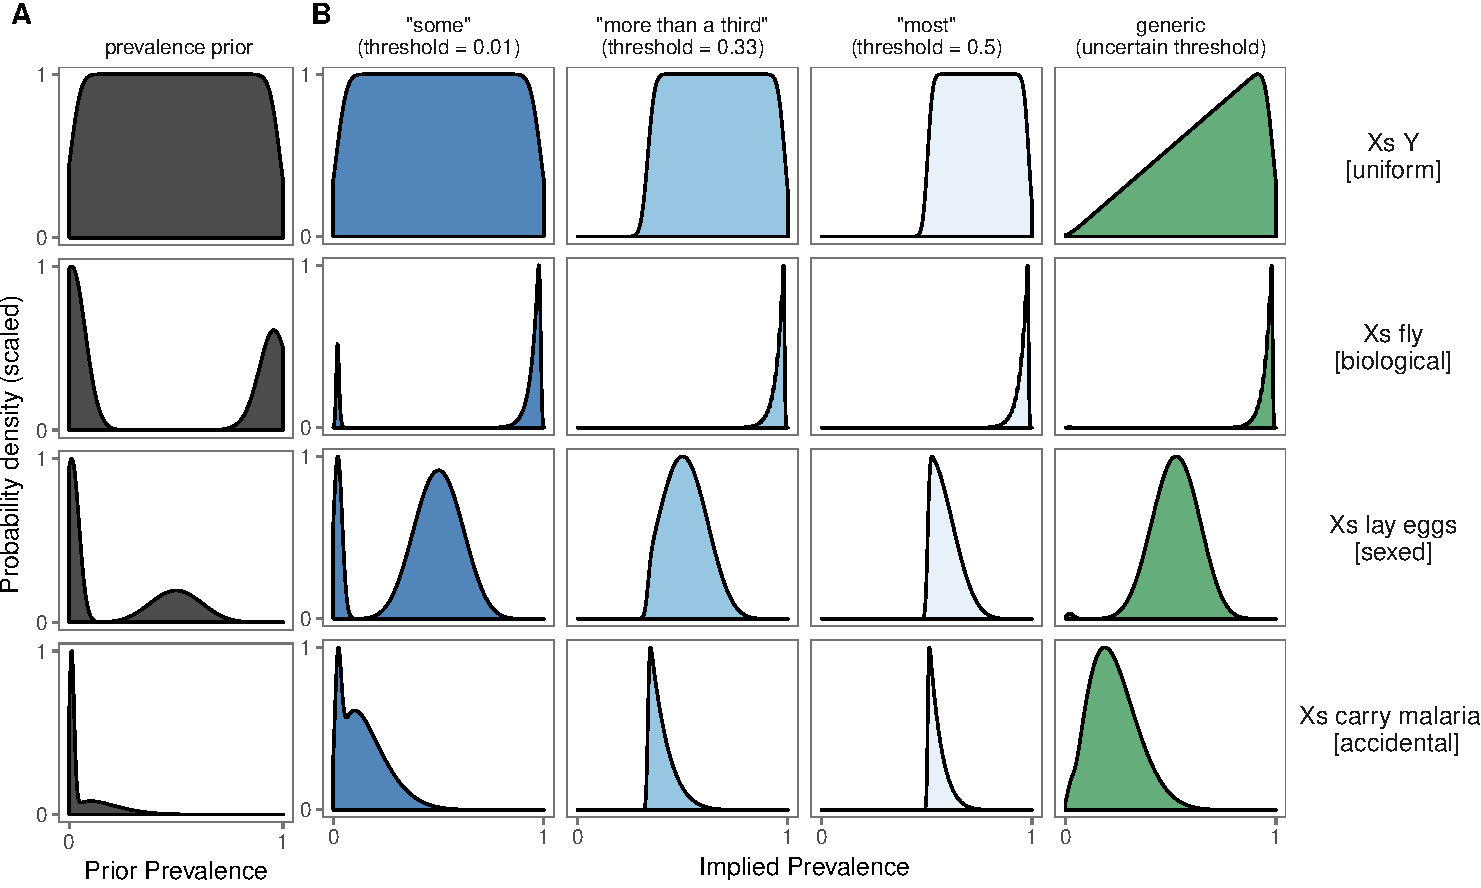
\includegraphics{genint_files/figure-latex/modelSimulations-1.pdf}
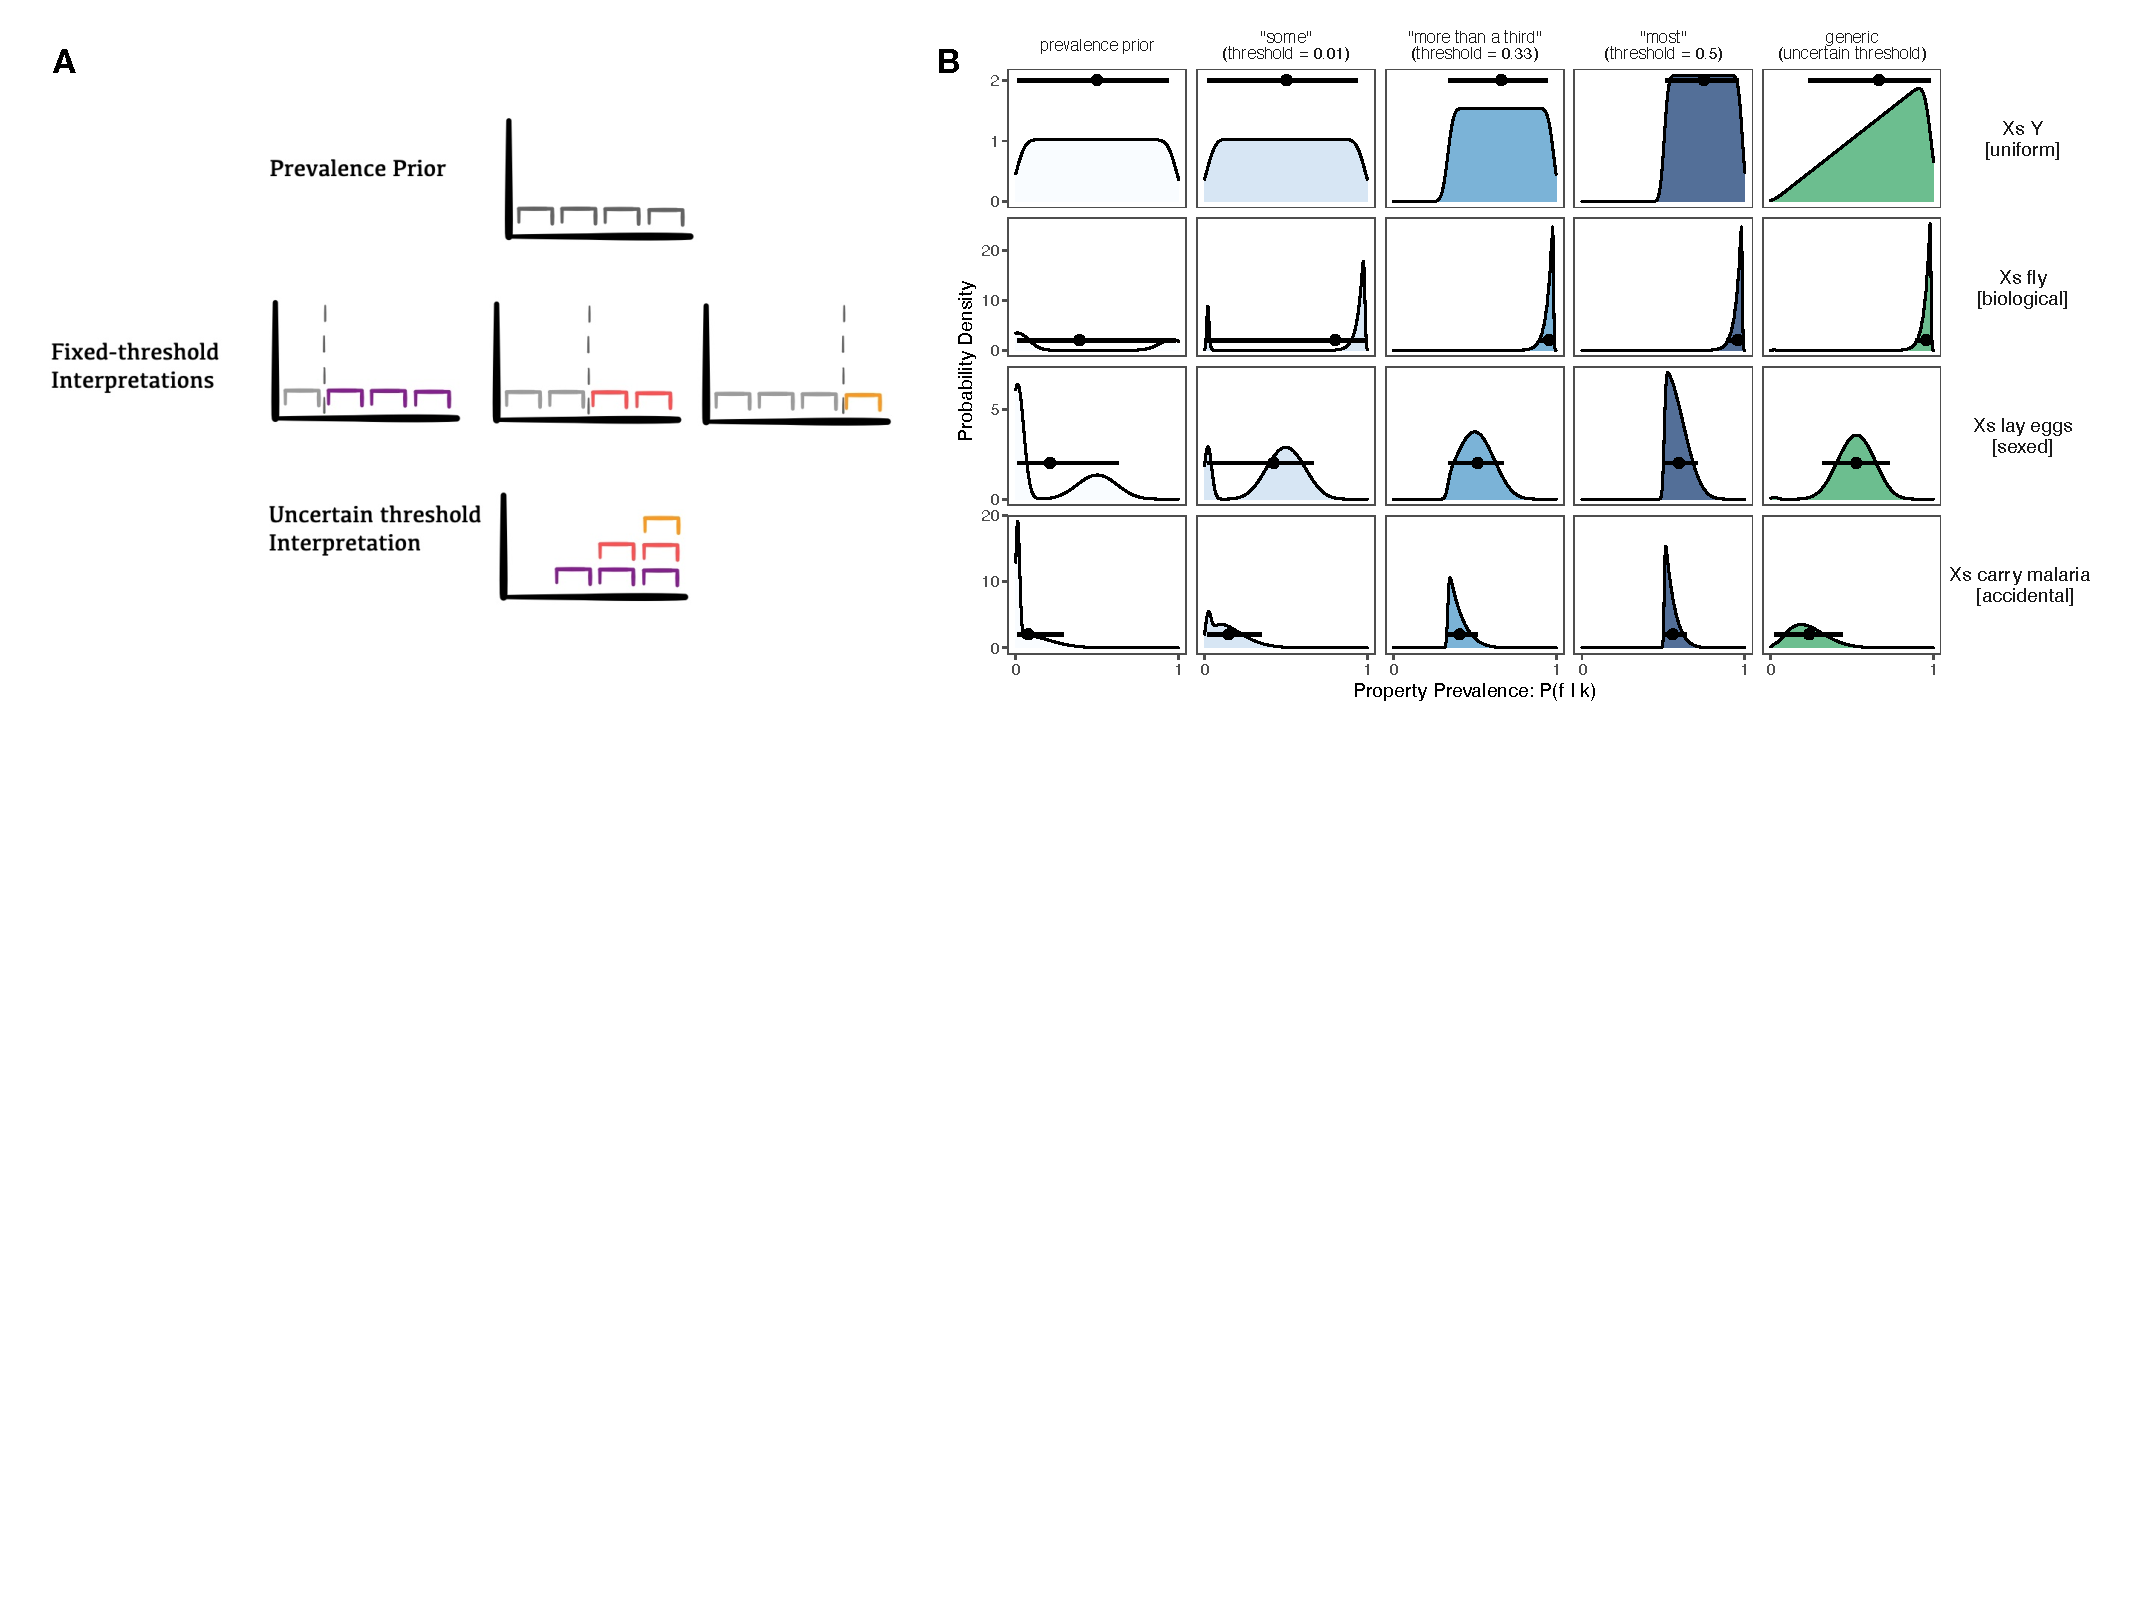
\includegraphics{figs/cartoon-model-sims}
\caption{\label{fig:modelSimulations}
Computational model overview.
A: Cartoon of belief updating in the case of a uniform prior over prevalence levels, according to the fixed-threshold and uncertain threshold models. Fixed-threshold models rule out prevalence levels below the threshold (light grey). The uncertain threshold model can be viewed as a composite of all the fixed-threshold models.
B: Comparison of uncertain threshold and fixed-threshold models for four different prevalence prior distributions, intuitively corresponding to different types of properties. Priors used for the four properties: $\textit{uniform} \sim \text{Beta}(1, 1); \textit{biological} \sim 0.6 \times \text{Beta}(1, 200) + 0.4 \times \text{Beta}(30, 1); \textit{sexed} \sim 0.6 \times \text{Beta}(1, 200) + 0.4 \times \text{Beta}(10, 10); \textit{accidental} \sim 0.6 \times \text{Beta}(1, 200) + 0.4 \times \text{Beta}(2, 10)$. Lines denote Bayesian 95\% highest density intervals and points denote means of distributions.
}
\end{figure}


\hypertarget{alternative-semantic-models}{%
\subsection{Alternative models}\label{alternative-semantic-models}}

We compare our uncertain threshold model to two sets of alternative models, which operate with the same prior beliefs, but which update them according to a different likelihood function. 

\subsubsection{Alternative semantics}

%Many empirical studies in psychology treat the ``statistical hypothesis'' about the meaning of a generic to be tantamount to a quantifier with a fixed threshold on prevalence, and consequently report evidence against this ``statistical hypothesis'' \cite{Prasada2006, Leslie2008, Cimpian2010, Khemlani2012, Prasada2013, Brandone2014}.
Many empirical studies in psychology consider a ``statistical hypothesis'' about the meaning of a generic, which is tantamount to a quantifier with a fixed threshold on prevalence \cite{Prasada2006, Leslie2008, Cimpian2010, Khemlani2012, Prasada2013, Brandone2014}.
We thus compare the uncertain threshold model to alternative models that update beliefs according to a fixed-threshold semantics (\emph{a la} quantifiers \emph{some} or \emph{most}). 
To isolate the contribution of the semantics model,  we endow the alternative models with the same background knowledge in the form of the prevalence prior distribution \(P(r)\).
Models with a fixed semantics are given by:
\begin{eqnarray}
%L_0^{some}(r \mid u) \propto  P(r \mid r > 0)  \label{eq:someModel}
P (r_{kf} \mid r_{kf} >  \theta^*) \propto \delta_{[r_{kf} > \theta^*]} \cdot P_f(r_{kf})  \label{eq:L0fixed}
\end{eqnarray}
If $\theta^* = 0$, then the model is analogous to a literal interpretation for \enquote{some}, which rules out the lowest possible prevalence level ($0\%$).\footnote{Note that a full model of quantifier interpretation would include their pragmatic interpretations (e.g., that \enquote{some} often implies \enquote{not all}). Such a model can be implemented in the same probabilistic modeling framework \cite{Goodman2013} but does not directly address our question of whether a fixed-threshold semantics is tenable for generics.} 
If $\theta^* = 0.5$, the model would be analogous to \enquote{most}, with a literal meaning meaning \emph{more than half}. 
Other fixed thresholds are possible as well (e.g., $\theta^* = 0.25$; \enquote{more than a quarter}).
Predictions of a few of these control models are shown in Figure~\ref{fig:modelSimulations}B.

A model that assumes a fixed threshold of $\theta^*$ places zero probability on any response less than $\theta^*$.
In case there are ratings in the experimental data sets that are less than $\theta^*$, we must supplement these models with an extrinsic noise process in order for this model to actually generate predictions for those data; that is, with some probability, were will assume participants respond at random.
This noise probability parameter will serve as an additional free parameter for the fixed-threshold control models. 
%We infer this noise probability parameter from the data for the fixed threshold models.

We additionally compare the generic interpretation models to a model that does not update beliefs, predicting prevalence ratings according to the prior distribution \(P(r)\).
This comparison informs us as to whether or not participants actually \emph{update} their beliefs when they hear a generic statement.

\subsubsection{Reified kinds}

Conceptual accounts of generics look beyond prevalence to model generic meaning \cite{Leslie2008, Cimpian2010, Khemlani2012, Prasada2013, Csibra2015}. This approach to looks to conceptual knowledge in the mind as the determining factor of the generic truth conditions (what makes them true or false). For the inverse problem --- learning from generic language --- these accounts would say that what is learned from a generic statement like \emph{Dogs bark} is that dogs ``are the kind of thing that bark'', where the property has some interpretation inside of a conceptual model of the world \cite<e.g., as a generic belief; >{Prasada2000}. This approach does not make direct predictions about how implied prevalence should vary as a function of property being predicated, so we take a step to formalize such a ``reified kinds'' view generics.

If there exists a predictable mapping between the meaning ``X is the kind of thing that Ys'' and prevalence, then the representation of prevalence (i.e., the prevalence prior) must be able to be partitioned into two clusters: the kinds that do possess Y and the kinds that do not possess Y. For example, if a prevalence prior is modeled as a mixture distribution (as in Figure \ref{fig:modelSimulations}B), then a straight-forward decision-rule for determining the prevalence implied by the generic would be to select the component of that mixture distribution which has the highest mean value. 
For example, if the prevalence prior can be partitioned into a mixture of two Beta distributions:
\begin{eqnarray}
P_f(r_{kf}) = \phi \cdot \text{Beta}(\gamma_1, \xi_1) + (1-\phi)\cdot \text{Beta}(\gamma_2, \xi_2)
% P (r_{kf} \mid u) \propto \cdot P_f(r_{kf})  \label{eq:kinds}
\end{eqnarray}

\noindent then the interpretation of the generic in terms of prevalence could simply be the Beta  distribution that has the higher mean.

\begin{eqnarray}
%P_f(r_{kf}) = \phi \cdot \text{Beta}(\gamma_1, \xi_1) + (1-\phi)\cdot \text{Beta}(\gamma_2, \xi_2)
P (r_{kf} \mid u) \propto  \begin{cases}
\text{Beta}(\gamma_1, \xi_1) \text{ if } \gamma_1 > \gamma_2 \\
\text{Beta}(\gamma_2, \xi_2) \text{ if } \gamma_2 > \gamma_1 
 \end{cases} \label{eq:rk}
\end{eqnarray}
\noindent where $\gamma$ represents the mean of the Beta distribution.
%
%
%\hypertarget{pragmatic-enrichment}{%
%\subsection{Pragmatic enrichment}\label{pragmatic-enrichment}}
%
%Even if the literal contribution of a generic sentence is modeled as a vague quantifier with a uniform prior on the threshold as Tessler and Goodman (2019) posit, the inferences a listener derives from a generic could quantitatively deviate from  the predictions of Eq.~\ref{eq:L0} by listeners taking into account the communicative intent of a speaker  (Clark, 1996; Grice, 1975; Levinson, 2000; Figure \ref{fig:cartoon}).
%Reasoning about why a speaker chooses to produce a generic could result in strengthened inferences, where the listener takes the generalization to apply more broadly than what a literal Bayesian reasoner would infer. 
%%That is, a listener could reason about why the speaker choose to produce a generic utterance (when they could have stayed silent)
%We model pragmatic reasoning by incorporating our model of literal generic interpretation (Eq.~\ref{eq:L0}) as a \emph{literal listener} model in the Rational Speech Act framework (Frank \& Goodman, 2012).
%In such a model, a listener \(L_1\) interprets an utterance $u$ by reasoning about a speaker \(S_1\) intentionally producing the utterance to update the beliefs of the literal listener \(L_0\):
%
%
%Equations \ref{eq:S1} \& \ref{eq:L1} are a vanilla Rational Speech Act model which has been used to account for a number of diverse pragmatic language understanding phenomena (for a review, see Goodman \& Frank, 2016; for a tutorial, see Scontras, Tessler, \& Franke, 2018).
%Equation \ref{eq:S1} is a model of a softmax rational agent deciding whether or not to produce an utterance in order to convey information to a literal listener $L_0$  (as defined in Equation \ref{eq:L0}), while taking into account the cost of producing the utterance (e.g., longer utterances are more costly to produce).
%
%
%Equation \ref{eq:L1} is a model of a pragmatic listener who understands that the generic utterance was produced by an intentional speaker \(S_1\) (Figure \ref{fig:cartoon}).
%Again, interpretations are strongly driven by the prevalence priors (Figure \ref{fig:tripartite}C). 
%However, pragmatic reasoning allows the utterances to imply stronger generalizations than literal interpretation because a speaker might not have bothered to produce the generic if the prevalence was not sufficiently high, especially if the speaker incurred some cost in producing the utterance (compare Figure~\ref{fig:tripartite}A~vs.~\ref{fig:tripartite}C).
%The differences between literal and pragmatic interpretations are most pronounced for priors with more uncertainty, such as the uniform prior. 
%We design our items in Expt.~1 to elicit a wide range of implied prevalence ratings in order to have sufficient quantitative variability to distinguish the predictions of the literal~vs.~pragmatic models.
%For purposes of quantitative modeling, we allow both the cost of the generic---\(\text{cost}(generic)\)---and the speaker's rationality parameter \(\alpha\) to be free parameters that we infer from the behavioral data.


%\hypertarget{the-influence-of-prevalence-priors-and-pragmatic-reasoning}{%
%\subsection{The influence of prevalence priors and pragmatic reasoning}\label{the-influence-of-prevalence-priors-and-pragmatic-reasoning}}





%Interpreting a generic sentence as providing a single positive observation to the listener provides a way to understand generics in a highly property-specific manner.
%Listeners may derive a stronger interpretation of a generic, however, by reasoning about the communicative nature of the sentence they hear
%That is, a generic sentence is produced by a speaker who has the goal of conveying information to them.
%Figure~\ref{fig:tripartite} shows the predictions of each level of recursion in the pragmatic interpretation model (Eqs.~\ref{eq:L0}, \ref{eq:S1}, \ref{eq:L1}).
%The speaker model (Eq.~\ref{eq:S1})  decides to produce the generic by reasoning about whether to convey to the literal listener the distribution implied by the generic~vs.~the prevalence prior, which results from staying silent (or producing the ``null'' utterance; Figure~\ref{fig:tripartite}A).
%The speaker production probabilities thus strongly depend on the prevalence prior as well as the assumed cost of production (Figure~\ref{fig:tripartite}B).
%The pragmatic listener reasons that a speaker would only produce the generic at relatively high prevalence levels (\emph{relative} to the prevalence prior) and thus the fact that the speaker bothered to say the generic implies even higher prevalence than the literal meaning implies. 
%This inference is strengthened as the cost of the utterance increases, though in a way that respects the prevalence prior (i.e., not all generics can imply 100\% prevalence, even given high cost to the utterance; Figure~\ref{fig:tripartite}C).

%When learning about an abstract property with a uniform prevalence prior (top row), the pragmatic model infers more strongly that at least most of the category have the property.
%For the other prevalence priors, the pragmatic model predicts lower-variance interpretations.
%We design Experiment 1 with a diverse stimulus set to elicit a wide range of variability in interpretations that could distinguish the literal from the pragmatic generic interpretation models.

%{\textcolor{Green}{[ndg: note: i changed "context" to other things (eg "property") in a bunch of places because what we're talking about is differences in target property and it's corresponding background knowledge. this is context in some sense, but i worry it would confuse people with more pragmatic / situated notions of context.]}}





\hypertarget{overview-of-experiments}{%
\section{Overview of Experiments}\label{overview-of-experiments}}

Our models of generic interpretation predict that the interpretations of generics should vary with the prevalence prior for the property in question.
Experiment 1 is a large scale version of \citeA{Cimpian2010}'s \emph{implied prevalence} task, with sufficiently dense measurements on the by-item level to reveal graded, quantitative variability among interpretations of generics of different properties. 
Experiment 2 is a replication and extension of \citeA{Cimpian2010}'s result that implied prevalence varies between generics about biological properties (in particular, body parts with color modifiers e.g., \emph{yellow fur}) and accidental properties (e.g., \emph{fungus-covered claws}).
%; this study serves to validate that the paradigm can elicit fine-grained quantitative variability, which we will build on to test the computational models.
%\citeA{Cimpian2010} reported differences 
%Our Preliminary Experiment 
Experiment 3 is a test of the causal influence of prevalence priors on generic interpretation, in which we manipulate participants' subjective prevalence priors.

Each of our experiments is divided into two parts. 
In Part A (Expts.~1a, 2a, 3a), we measure participants' prior beliefs about the prevalence of the features used in our stimuli (e.g., the prior probabilities of different levels of prevalence of the feature \emph{likes to cuddle}). %; we do this by asking about the prevalence of the feature among a variety of alternative, familiar categories (e.g., \emph{what percentage of \{cats, mice, elephants, ...\} like to cuddle?}).
In Part B (Expts.~1b, 2b, 3b), we measure the prevalence implied by a generic about a novel categories (e.g., \emph{Dorbs like to cuddle.}). 
We then perform a series of quantitative analyses aimed at predicting the prevalence implied by the generic (Part B) from the prior distribution of prevalence (Part A), assuming different models of belief-updating from a generic (i.e., likelihood functions that update a prior distribution into a posterior distribution on prevalence). 
The comparison of different formal models of generic interpretation using the same elicited prior knowledge allows us to provide evidence for a particular model of generic interpretation, while precisely articulating the effect of prior knowledge. 

The sample size, exclusion criteria, and planned statistical contrasts for Expts.~1 \& 3 were pre-registered on the Open Science Framework.
All cognitive and Bayesian data analytic models were implemented in the probabilistic programming language WebPPL \cite{dippl}. 
All data, analysis scripts, models, and links to experiments and pre-registration reports can be found at \url{www.github.com/mhtess/generic-interpretation}.

\hypertarget{experiment-1}{%
\section{Experiment 1: Variability in Generic Interpretation}\label{experiment-1}}

This experiment is designed to test models of generic interpretation by measuring the prevalence implied by a generic about a novel kind, using a diverse set of properties.
We first elicit participants' prior beliefs about the likely prevalence levels expected for these properties (Expt. 1a).
We then use the elicited prevalence priors to make model predictions about the prevalence implied by a generic (Expt. 1b).

\hypertarget{experiment-1a-prevalence-prior-elicitation}{%
\subsection{Experiment 1a: Prevalence prior elicitation}\label{experiment-1a-prevalence-prior-elicitation}}

In this experiment, we elicit prior beliefs about prevalence for a diverse set of properties.
These prior beliefs will be used inside the computational models in order to predict interpretations of generic statements about novel categories. %(akin to Expt.~1). 
Because the properties are familiar properties, we can elicit participants' knowledge by asking about the property among familiar  categories.

\hypertarget{methods}{%
\subsubsection{Methods}\label{methods}}

\hypertarget{participants-1}{%
\paragraph{Participants}\label{participants-1}}

We recruited 200 participants from MTurk.
This number was arrived at with the intention of getting approximately 23 independent sets of ratings for each unique item in the experiment, which corresponds to roughly 115 ratings per item.
Participants were restricted to those with U.S. IP addresses and with at least a 95\% MTurk work approval rating (these same criteria apply to all experiments reported).
The experiment took on average 7 minutes and participants were compensated \$0.80.

\hypertarget{materials}{%
\paragraph{Materials}\label{materials}}
We created a stimulus set composed of seventy-five properties.
Items were generated by the first author by considering eight different classes of properties: physical characteristics (e.g., \emph{have brown spots}, \emph{have four legs}), psychological characteristics (e.g., \emph{experience emotions}), dietary habits (e.g., \emph{eat human food}), habitat (e.g., \emph{live in zoos}), disease (e.g., \emph{get cancer}, \emph{carry malaria}), reproductive behavior (e.g., \emph{have a menstrual cycle}), aggressive behaviors (e.g., \emph{pound their chests to display dominance}, \emph{hunt other animals}), and other miscellaneous behaviors (e.g., \emph{perform in the circus}, \emph{sing beautiful songs}); online sources about strange animal behaviors were consulted in order to find the more obscure properties. Full list of materials can be found in Table B.1 in Appendix B.

\hypertarget{procedure-and-materials-1}{%
\paragraph{Procedure and materials}\label{procedure-and-materials-1}}
The task comprised two different kinds of trials: a category elicitation trial, which appeared first, and twelve prevalence elicitation trials, which used the responses generated in the category elicitation trial.
In the category elicitation trial, participants were asked to list three kinds of animals for each of five different classes of animals: mammals, fish, birds, insects/bugs, amphibians/reptiles.
The five classes of animals were presented in a randomized order on the screen and there were three text boxes for each in which participants could type an animal kind.

On the subsequent prevalence elicitation trials, participants were shown a random subset of five of the animal kinds they generated on the initial trial and asked, for each of these categories, what percentage of the category they believed had a property (e.g., \enquote{Out of all of the cheetahs in the world, what percentage do you think attack hikers?}).\footnote{Pilot results indicated similar responses were generated by a question about frequency (e.g., \enquote{Out of 100 cheetahs, how many do you think attack hikers?}).} 
Participants responded using a slider bar with endpoints labeled 0\% and 100\%, and the exact number corresponding to their slider bar rating was displayed once participants clicked on the slider bar.
Each participant saw a random selection of twelve properties.

As an attention check, at the end of the prevalence elicitation trials, participants were asked to select, from a list of ten, all of the properties they could remember being tested on.
The list included five properties that they had been tested on and five distractors.

\hypertarget{results}{%
\subsubsection{Results}\label{results}}
We used the same exclusion criteria that were preregistered for the subsequent generic interpretation study: \url{https://osf.io/bwn4t/register/5771ca429ad5a1020de2872e}.
Participants who did not have at least 4 out of 5 hits and at least 4 out of 5 correct rejections during the memory trial were excluded (\(n = 15\)).
In addition, we excluded participants who self-reported a native language other than English (\(n = 13\)).
This left a total of \(n = 175\) participants, with items receiving on average 28 (range = {[}16, 38{]}) sets of participant responses, for a total of on average 140 ratings (range = {[}80, 190{]}) since each participant provided five ratings.

The prevalence prior distribution can be thought of as describing the expectations about the prevalence of a feature for a novel category that a person has yet to experience. 
A response in this task can be thought of as a sample from a property's prevalence prior distribution and thus, the distribution of responses for an item are a sample-based approximation of the prevalence prior distribution (Figure~\ref{fig:genInt-prevPrior}A). 
%Tshows these distributions of responses for ten example items.
For example, given participants' knowledge of familiar categories, a learner would expect the property \emph{has four legs} to be either completely universal (prevalence = 100\%) or completely absent (prevalence = 0\%) in a novel category.
The distribution for the property \emph{eats insects} looks similar, though there is considerable probability mass spread among the non-binary alternatives (\(0\% <\) prevalence \(< 100\%\)).
\emph{Get in fights with other animals} is similar but has substantially less probability mass at 100\% prevalence: It is unlikely that this property is widespread in a category.
\emph{Live in urban areas} shows a monotonically decreasing probability function; even if this property is present in a category, it is unlikely to be highly prevalent. 
\emph{Live in zoos} is expected to be even less prevalent, and the property \emph{has seizures} is expected to even more rare.
Some prevalence prior distribution exhibit unique structure; for instance,  the property \emph{gets erections} is only expected to be present in 50\% of the population when it is present at all because of the fact that this is a property that only male members of categories can possess. In this way, theory-based considerations can influence the structure of these prevalence priors (see also \citeNP{Tessler2019psychrev} for a discussion of this relationship). 

Most of the elicited prevalence prior distributions appear at least bi-modal.
To visualize all properties simultaneously, we represent each distribution by two statistics: the relative probability mass at 0\%---\(P(\text{feature is present})\), or \(P(r > 0)\)---and the expected value (mean) of the distribution conditional on the prevalence being greater than 0\%---\(\mathbb{E}[P(r \mid r>0)]\) or the property's \emph{prevalence when present}.
The $P(\text{feature is present})$ is a measure of the (inverse-)distinctiveness of the feature (i.e., among how many animal categories is the property expected to be present). 
\emph{Prevalence when present} is the average prevalence among the categories for which the property \emph{can} occur. 
Figure~\ref{fig:genInt-prevPrior}B shows the distributions of these two parameters: The stimulus set covers a wide range of possible values of both of these parameters.
This suggests we have sampled items with priors that exhibit a lot of quantitative variability, as desired.

To confirm the multi-modality of the empirical prior distributions, we conduct a Bayesian analysis where we model the prior elicited data (on a by-item basis) as being generated from some combination of mixtures of Beta distributions.\footnote{We use Beta distributions to match the form of the response variable: a number between 0 - 1.} 
We compare the likelihood of the prior elicited data, modeling each item independently, under a single Beta distribution as well as  mixtures of 2-, 3-, and 4- Beta distributions; this comparison allows us to determine the best functional form of the priors, which will be useful when we try to model both the prior data and the generic interpretation data simultaneously. 
The method of model comparison we employ---Bayes Factors---averages across all values of any free parameters of the model (weighted by their prior probabilities) and thus,  penalizes models with extra free parameters if, in fact, the model's predictions are not greatly improved by the addition of free parameters (or, are highly sensitive to the exact values of those parameters).
Each prevalence prior component (i.e., each Beta distribution) has two parameters governing its shape: a mean \(\gamma\) and variance parameter \(\xi\); in addition, for models that use mixtures of 2-, 3-, or 4-Beta distributions, we have an additional 1, 2, or 3 parameters (respectively) governing the relative contribution (i.e., the weight) of each mixture component. 
We put uninformative priors over these parameters \(\gamma \sim \text{Uniform}(0, 1)\), \(\xi \sim \text{Exponential}(1)\), \(\phi \sim \text{Dirichlet}([1]^n)\) and compute the marginal likelihood of the data by using an Annealed Importance Sampling algorithm \cite{neal2001annealed} implemented in the probabilistic programming language WebPPL.
We find that the most parsimonious account of the prior elicited data is that of a mixture of two Beta distributions (log Bayes Factors of 2-vs.1-Beta: $\log \text{BF}_{2,1}= 
\rlgetnum{expt1a_mixture_of_betas_bf.csv}{n_components}{1}{log_bf}{0}$; 2-~vs.~3-Betas: $\log \text{BF}_{2,3}= 
\rlgetnum{expt1a_mixture_of_betas_bf.csv}{n_components}{3}{log_bf}{0}$; 2-~vs.~4-Betas: $\log \text{BF}_{2,4}= 
\rlgetnum{expt1a_mixture_of_betas_bf.csv}{n_components}{4}{log_bf}{0}$).
Thus, we will assume the prevalence prior data follows a mixture of 2-Beta distributions when we jointly model the generic interpretation data, which we measure in our next experiment.  

%Given these priors, our model makes quantitative predictions about the prevalence implied by a novel generic sentence (e.g., \enquote{Lorches live in zoos}), which we test in Experiment 1b.

\begin{figure}
\centering
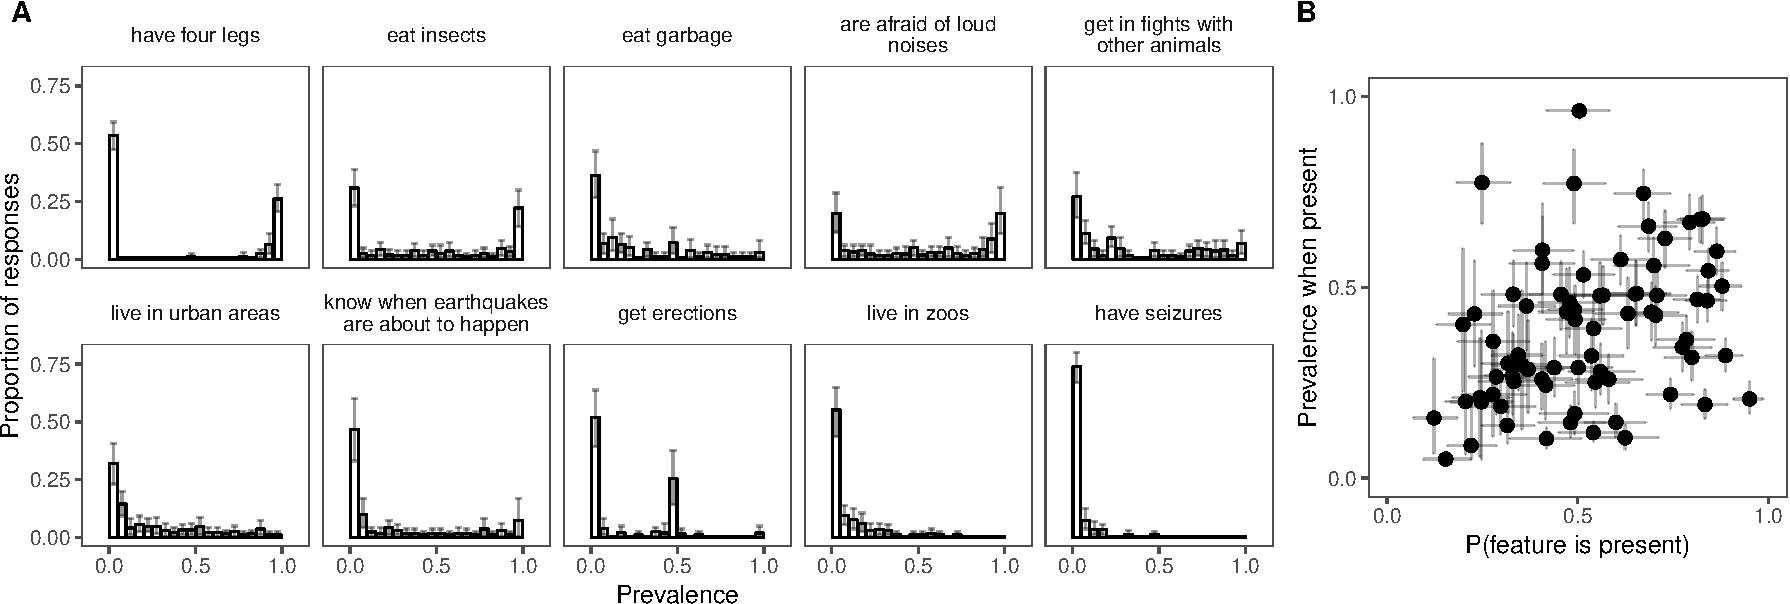
\includegraphics{genint_files/figure-latex/genInt-prevPrior-1.pdf}
\caption{\label{fig:genInt-prevPrior}Prevalence priors for a diverse set of animal properties. A: Ten example prevalence priors elicited in Expt. 2a. Distributions vary in terms of how rare the property is across categories (probability mass at 0\% prevalence) as well as the prevalence within a category where the property is present (shape of non-0\% part of the distribution). B: Prevalence priors summarized by their relative probability mass at zero-prevalence P(feature is present), and their expected value among non-zero prevalence levels: Prevalence when present. The stimulus set covers a wide range of possible values of both of these parameters. Error bars denote bootstrapped 95\% confidence intervals.}
\end{figure}

\hypertarget{experiment-1b-generic-interpretation}{%
\subsection{Experiment 1b: Generic interpretation}\label{experiment-1b-generic-interpretation}}

\hypertarget{methods-1}{%
\subsubsection{Methods}\label{methods-1}}

\hypertarget{participants-2}{%
\paragraph{Participants}\label{participants-2}}
%
We recruited 200 participants from MTurk.
This number was arrived at with the intention of getting approximately 50 ratings for each unique item in the experiment.\footnote{The intended number of ratings in this experiment is smaller than the corresponding number of ratings in the prior elicitation task (Expt.~1a), which was approximately twice as many. In the prior task, we were eliciting multimodal distributions, which require more samples  to approximate faithfully than unimodal distributions, which we anticipated for this generic interpretation task.}
The experiment took on average 5.50 minutes and participants were compensated \$0.80.

\hypertarget{procedure-and-materials-2}{%
\paragraph{Procedure and materials}\label{procedure-and-materials-2}}
%
The materials were the same as in Expt. 1a.
Participants were told that scientists had recently discovered lots of new animals that we did not know existed.
On each trial, they would be told facts about the new animals and be asked to translate it into the percentage of that animal to which it applies.
On each trial, participants read \enquote{You are told: \emph{generic}}, where the generic sentence was a bare plural statement about a familiar property \(F\) applying to a novel animal category \(K\) (e.g., \emph{Javs attack hikers}).

Participants were then asked \enquote{Out of all of the \emph{K}s on the planet, what percentage do you think \emph{F}?} (e.g., \enquote{Out of all of the javs on the planet, what percentage do you think attack hikers?}).
Participants responded using a slider bar with endpoints labeled 0\% and 100\%, and the exact number corresponding to their slider bar rating was displayed once participants clicked on the slider bar.
This kind of explicit question about prevalence has been used to reveal differences in the interpretations of generics~vs.~quantified statements in adults and young children \cite{Gelman2002, Brandone2014} as well as differences in interpretations of generics about different properties \cite{Cimpian2010}. 
It is not a measure of unconscious probabilistic expectations, which can often deviate from this kind of conscious probabilistic judgment \cite<e.g.,>{wu2017asking}.\footnote{
It has been observed, however, that that probabilistic information conveyed using perceptual features (e.g., spatial extent) can lead to better understanding of probabilities, as measured by performance on a probabilistic search task \cite{wu2017asking}.
Thus, our use of a perceptually-grounded slider bar could support participants' estimations of probability and bring more alignment between unconscious probabilistic expectations and participants' reported prevalence values.
%The \citeA{wu2017asking} task is only indirectly comparable, however, because it concerns the comprehension of probabilistic information whereas we examine the reporting of probabilistic information.
}
Though the response measure may encourage some amount of gradience in responses \cite<cf.,>{armstrong1983some}, the fact that the numeric rating appears above the slider bar allows participants to provide an exact rating should they desire. 

Novel animal category names were mostly taken from Cimpian et al. (2010) and similar studies on generic language.
Each participant completed thirty-five trials, corresponding to a random subset of the full stimulus set.
After the generic interpretation trials, participants completed the same memory check trial as was done in the prior elicitation.
They were shown ten properties and asked to click on those they had seen in the experiment.
Following the memory check trials, participants completed up to five explanation trials, depending on their ratings in the task.
On an explanation trial, participants saw a rating they had given for a property they had rated as applying to less than 50\% and asked if they could explain why they gave the response that they gave.
Participants also had the option of changing their response after providing an explanation.
These data were only used in exploratory analyses and not for the main analyses reported below.
If participants gave no ratings less than 50\%, they did not complete any explanation trials.

\hypertarget{descriptive-results}{%
\subsubsection{Descriptive results}\label{descriptive-results}}

We used preregistered exclusion criteria, which were also used for Expt. 1a.
Participants who did not have at least 4 out of 5 hits and at least 4 out of 5 correct rejections during the memory trial were excluded (\(n = 62\)).
In addition, we excluded participants who self-reported a native language other than English (\(n = 8\)).
This left a total of \(n = 132\) participants, with items receiving on average 62 responses (range = {[}50, 77{]}).

%As in the replication of \citeA{Cimpian2010}, 
We observe a clear gradient in the implied prevalence ratings across our seventy-five items (Figure~\ref{fig:genint-empiricalData}).
On one end of the continuum, the generic \emph{Wugs have four legs} is interpreted as a universal (applying to exactly 100\% of wugs) by half of participants (36 out of 70) and which received a mean implied prevalence rating of 0.96 (95\% confidence interval: [0.93, 0.98]).\footnote{Note the novel category term is randomized for each participant and property. We use particular novel category terms in the text for ease of exposition.}
On the other end of the spectrum is \emph{Glippets perform in the circus}, which is interpreted as applying to less than 25\% of glippets by over half of participants (35 out of 61) and which receives a mean rating of 0.31 [0.23, 0.39].
Additionally remarkable is the distribution of responses for individual items: Though \emph{Feps live in zoos} is taken by many participants to mean that around 25\% of feps live in zoos, others take it to mean that almost 100\% live in zoos; such variability in interpretation is not unreasonable: some animal categories (e.g., Micronesian Kingfishers) exist entirely in zoos, while others do not.
In addition to the extreme endpoints, we find average ratings at all levels of prevalence in between, even for predicates that have the same main verb (e.g., \emph{live in} \emph{trees}~vs.~\emph{live in urban areas}~vs.~\emph{live in high-rise buildings}~vs.~\emph{live in zoos}; compare also properties involving the verb \emph{eat}; Figure~\ref{fig:genint-empiricalData}), arguing against a view that variability can be traced back simply to verbs with different ``generalizing powers'' \cite{Abelson1966, Cimpian2010}.
This extreme gradience also stands in contrast to the results of \citeA{Cimpian2010}, which left open the possibility that were just a few special distinctions of properties that had unique implied prevalences (e.g., biological~vs.~accidental properties; see also Figure \ref{fig:cimpian-modelingResults}). 
Explaining the extreme gradience we observe in our data set requires a quantitative theory. 

%\ndg{emphasize the gradience, in contrast with cimpian results which left open the possibility that there were just a few categories... this means we really want a quant model.}

To determine whether the variability we observe can be traced back to difference in how individual participants' use the slider bar (e.g., how extreme or moderate a participants is in their usage of the slider bar ratings), we normalized each participant's ratings by subtracting the mean and dividing by the standard deviation of that participant's responses. We then compared the mean normalized ratings by-item to the mean unnormalized (original) ratings by-item. We find an extremely strong correlation between the two (r = 0.9947), which suggests that the gradience in mean ratings we observe by-item is not driven by individuals’ variability in how extreme or moderate their responses are.

To assess the reliability of these data, we ran a replication (\(n=140\)) using a slightly different dependent measure.\footnote{By experimenter error, only seventy-four of the seventy-five items were collected in the replication data set.}
Instead of being asked a question about percentages (e.g., \enquote{Out of all of the Ks in the world, what percentage F?}), participants were asked a question in terms of frequency: \enquote{Out of 100 Ks, how many do you think F?}.
The empirical by-item means between these data and the original data are highly correlated (\(r(74) = 0.96\), \(r_{spearman}(74)= 0.96\)), indicating very high data reliability.

We also see evidence of quantization of responses, especially around 50\% prevalence. The quantization can be observed at 5\% increments and is likely due to the fact that the slider bar displayed the exact percentage above the slider bar and that people prefer round numbers. 
In our model-based analysis below, we discretize the state space to increments of 5\%, and this quantization does not change any of theoretical conclusions we will draw.


\begin{figure}
\centering
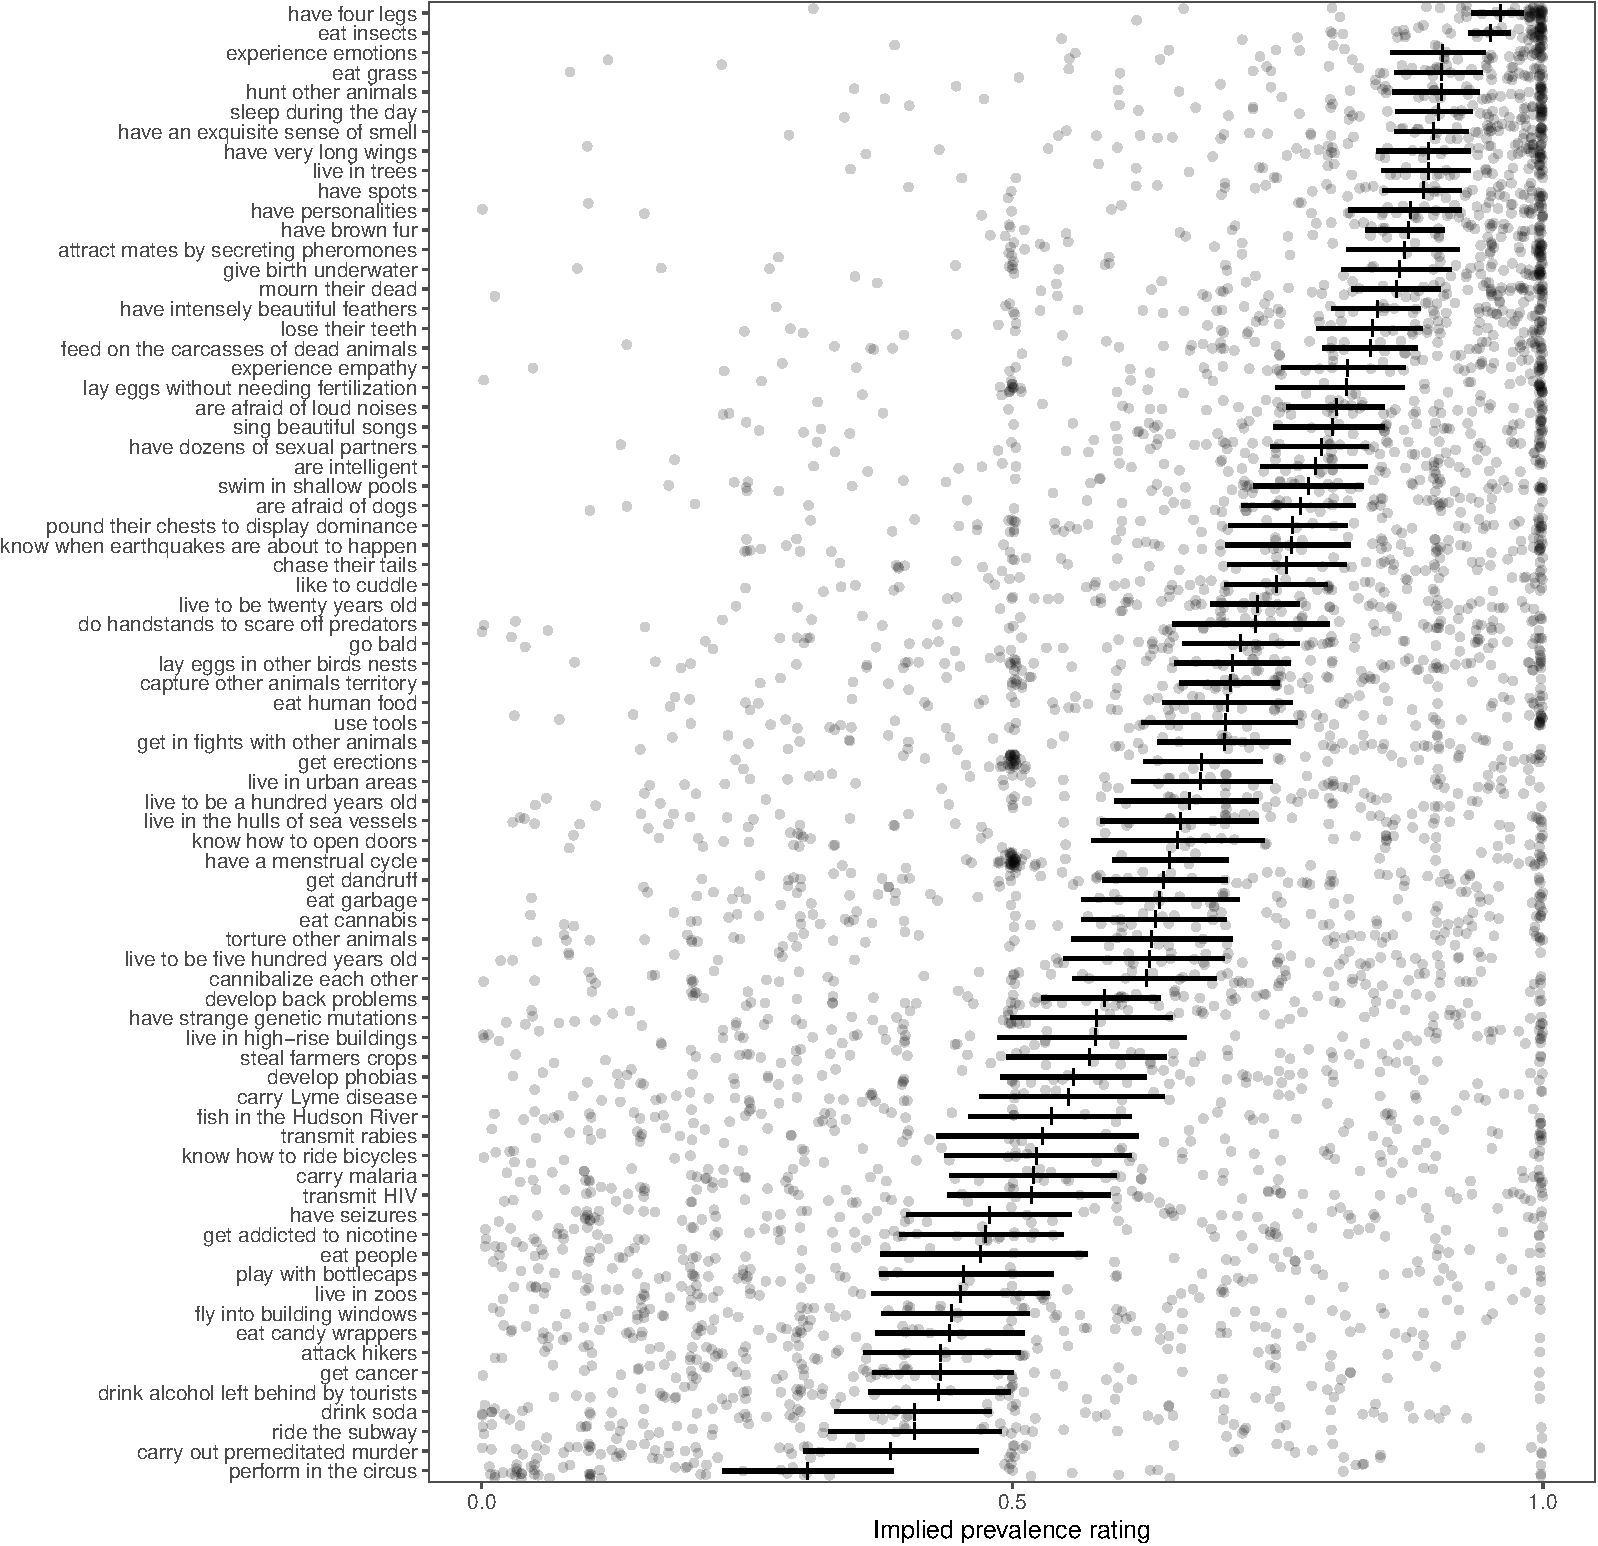
\includegraphics{genint_files/figure-latex/genint-empiricalData-1.pdf}
\caption{\label{fig:genint-empiricalData}Implied prevalence ratings for a diverse set of seventy-five items. Vertical lines denote means, points are individual empirical judgments. Error bars denote bootstrapped 95\% confidence intervals.}
\end{figure}


\hypertarget{model-based-analyses}{%
\subsubsection{Model-based analyses}\label{model-based-analyses}}

Our model-based analyses ask how well the various models for the meaning of a generic accommodate the human generic interpretation data and provides the most parsimonious view of the data.
We compare our uncertain threshold model to fixed-threshold models for fixed-threshold values between 0\% and 60\% (e.g., fixed-threshold at 0\% is analogous to the quantifier ``some''; fixed-threshold at 50\% is analogous to the quantifier ``most''). 
We additionally compare to a ``best'' fixed-threshold model, where the model's semantic threshold is a global, free parameter inferred from the data. 
Finally, we include a comparison to a formalization of a ``reified kinds'' control model, where what the generic does is pick out the component of the prior distribution which has the higher mean level of prevalence. 
Since fixed-threshold models assign 0-probability to all levels of prevalence below the threshold, these models must be supplemented with the extrinsic noise process (e.g., random guessing).
We estimate the noise parameter and all other model parameters using Bayesian methods in order to determine the most likely values of the latent parameters given our hypotheses about how both the prior elicitation and generic interpretation data were generated.\footnote{Appendix C in \citeA{Tessler2019psychrev} provides a careful analysis of the behavior of this joint Bayesian inference strategy for jointly modeling the prevalence prior parameters together with other parameters of the model governing generic interpretation. They find imperceptibly small differences between the parameters inferred from the prevalence prior data in isolation and those inferred by jointly modeling the prior elicitation together and the generic interpretation data, suggesting that in order to provide a stronger quantitative fit to the generic interpretation data, the prevalence priors are not significantly distorted by this method.}
%That is, we ask if there is some reasonable setting of the prevalence priors \ndg{"setting of the prevalence priors" dosn't exactly make sense to me...} that, together with a particular model of generic interpretation, could give rise to the generic interpretation results.
We compare the uncertain threshold model to the fixed-threshold + noise models and the reified kinds model using the standard Bayesian model comparison metric: marginal likelihoods, or Bayes factors \cite{LeeWagenmakers2014}.

%For data analysis, we assume that the prevalence priors take the form of a three-component mixture of Beta distributions\footnote{We use Beta distributions to match the form of the response variable: a number between 0 - 1.}, whose parameter uncertainty is strongly constrained by data from our prior elicitation task.
%We posit uncertainty in the parameters governing the listener prevalence prior distribution.
%Our prior elicitation task helps constrain the values of the parameters of the prevalence priors, which we assume takes the form of a three-component mixture of Beta distributions model.
%\footnote{We use Beta distributions to match the form of the response variable: a number between 0 - 1.}

%The only other parameters we introduce are specific to certain generic interpretation models:
%The model that assumes a literal semantics identical to the quantifier \enquote{most} (threshold at 0.5) must be augmented with an extrinsic noise parameter in order to accommodate responses that are literally false under this interpretation of a generic (i.e., implied prevalence ratings below 0.5).
%The pragmatic generic interpretation model posits that listeners interpret generics by strengthening a literal meaning equivalent to a single positive example of the category with the communicative force of an utterance produced by an intentional speaker.
%This model thus has two additional free parameters: The implicit cost of producing a generic in comparison to staying silent (\emph{utterance cost}) and the degree of information-theoretic optimality with which the speaker behaves (\emph{speaker optimality}).


\hypertarget{model-definition-and-inference}{%
%\paragraph{Model definition and inference}
\label{model-definition-and-inference}}


%\begin{figure}[ht]
%  \begin{center}
%    \begin{tabular}{cc}
%\begin{tikzpicture}
%  \node[obs]          (d-c)   {$d^{gen}_{f,i}$}; %
%  \node[obs, left=3.5 of d-c, yshift=2cm]          (x)   {$d_{f, i'}^{prior}$}; %
%  \node[latent, above=1cm of x, xshift=-0.5cm] (mx) {$\phi^f$} ; %
%  \node[latent, above=2cm of x, xshift=0.75cm]  (sx) {$\gamma^f_j$} ; %
%  \node[latent, above=2cm of x, xshift=1.75cm]  (dx) {$\xi^f_j$} ; %
%%  \factor[above=of x] {x-f} {left:$\text{mixture of Betas}$} {mx, sx,dx} {x} ; %
%  \edge[above=of x]{mx, sx,dx} {x} ; %
%      \node[latent, right=2cm of x]  (xf)   {$r^{f}$}; 
%  \edge[above=of xf]  {mx, sx,dx} {xf} ; %
%
%  \node[det, above=0.52cm of d-c] (L1) {$L_1(r^f \mid u)$} ; % 
%   \node[latent, right=0.6cm of L1, yshift=0.5cm] (alpha) {$\alpha$}; %
%   \node[latent, right=0.6cm of L1, yshift=-0.5cm] (cost) {$c$}; %
%  \edge[-] {xf} {L1} ;
%  \edge[-] {alpha} {L1} ;
%  \edge[-] {cost} {L1} ;
%  \edge{L1} {d-c} ;
%
%\gate {RSAgate} {(L1)(xf)} {} ; %
%\node[text width=1cm] at (-1,2.75) {$RSA$};
%
%    \plate{gen-data}{
%    (d-c)
%  }{$i \in \mathcal{P}$}
%    \plate{prior-data}{
%    (x)
%  }{$i' \in \mathcal{P'}$}
%{
%\tikzset{plate caption/.append style={above right=5pt and 12pt of #1.north west}}
%\plate{mix} {
%(sx)(dx)
%}{$j \in \{1, 2\}$};
%}
%\plate{items}{
%(gen-data) (prior-data)
%(mx)(sx)(dx)(d-c)(x)(mix)(RSAgate)
%}{$f \in \mathcal{F}$}
%
%\node[draw, align=left, execute at begin node=\setlength{\baselineskip}{3ex}] at (7,4) { 
%$\alpha \sim \text{Uniform}(0,30) $\\
% $c \sim  \text{Uniform}(0,10) $ \\
% \\
%$\phi_f \sim \text{Uniform}(0, 1)$ \\
% $\gamma^f_j \sim \text{Uniform}(0, 1), \xi^f_j \sim \text{Exponential}(1)$ \\
%  $d^{prior}_{f, i'} \sim \phi^f \cdot \text{Beta}(\gamma^f_1, \xi^f_1) + (1-\phi^f) \cdot \text{Beta}(\gamma^f_2, \xi^f_2)$ \\
%    $r^f \sim \phi^f \cdot \text{Beta}(\gamma^f_1, \xi^f_1) + (1-\phi^f) \cdot \text{Beta}(\gamma^f_2, \xi^f_2)$ \\
%
% \\
%
%$ d^{gen}_{f, i} \sim L(r^f \mid u  = \text{generic}) = \int_{\theta} L(r^f, \theta \mid u) \diff \theta$
%};
%\node[draw, align=left, execute at begin node=\setlength{\baselineskip}{3ex}] at (6,0) {Rational Speech Act model\\ 
%$L_1(r^f, \theta \mid u) \propto S_1(u \mid r^f, \theta) \cdot P(r^f) \cdot P(\theta) $\\ 
%$S_1(u \mid r^f, \theta)\propto \exp{( \alpha \cdot [ \ln L_0(r \mid u, \theta) - c(u)])} $\\
%$L_0(r^f \mid u, \theta) \propto  \delta_{\denote{u}(r^f, \theta)} \cdot P(r^f)$
%};
%\end{tikzpicture}
%    \end{tabular}
%  \end{center}
%  \caption{Fully Bayesian data analytic approach.}
%  \label{fig:bayesnet}
%\end{figure}


\begin{figure}[ht]
  \begin{center}
    \begin{tabular}{cc}
\begin{tikzpicture}
  \node[obs]          (d-c)   {$d^{gen}_{f,i}$}; %
  \node[obs, left=3.5 of d-c, yshift=2cm]          (x)   {$d_{f, i'}^{prior}$}; %
  \node[latent, above=1cm of x, xshift=-0.5cm] (mx) {$\phi^f$} ; %
  \node[latent, above=2cm of x, xshift=0.75cm]  (sx) {$\gamma^f_j$} ; %
  \node[latent, above=2cm of x, xshift=1.75cm]  (dx) {$\xi^f_j$} ; %
%  \factor[above=of x] {x-f} {left:$\text{mixture of Betas}$} {mx, sx,dx} {x} ; %
  \edge[above=of x]{mx, sx,dx} {x} ; %
      \node[latent, right=2cm of x]  (xf)   {$r^{f}$}; 
  \edge[above=of xf]  {mx, sx,dx} {xf} ; %

  \node[det, above=0.52cm of d-c] (L1) {$L(r^f \mid u)$} ; % 
   \node[latent, right=1cm of d-c] (omega) {$\omega$}; %
   \node[latent, right=0.6cm of L1] (thetastar) {$\theta^*$}; %
%   \node[latent, right=0.6cm of L1, yshift=-0.5cm] (cost) {$c$}; %
  \edge[-] {xf} {L1} ;
%  \edge[-] {alpha} {L1} ;
%  \edge[-] {cost} {L1} ;
  \edge{L1} {d-c} ;
    \edge{omega} {d-c} ;
    \edge{thetastar} {L1} ;


\gate {RSAgate} {(L1)(xf)} {} ; %
\node[text width=1cm] at (-1.5,1.25) {\emph{\small{Cognitive model}}};

    \plate{gen-data}{
    (d-c)
  }{$i \in \mathcal{P}$}
    \plate{prior-data}{
    (x)
  }{$i' \in \mathcal{P'}$}
{
\tikzset{plate caption/.append style={above right=5pt and 12pt of #1.north west}}
\plate{mix} {
(sx)(dx)
}{$j \in \{1, 2\}$};
}
\plate{items}{
(gen-data) (prior-data)
(mx)(sx)(dx)(d-c)(x)(mix)(RSAgate)
}{$f \in \mathcal{F}$}

\node[draw, align=left, execute at begin node=\setlength{\baselineskip}{3ex}] at (7,5.5) { 
%$\alpha \sim \text{Uniform}(0,30) $\\
% $c \sim  \text{Uniform}(0,10) $ \\
 $\omega \sim  \text{Uniform}(0, 1) $ \emph{[fixed threshold models only]}\\
  $\theta^* \sim  \text{Uniform}(0, 1) $ \emph{[``best'' threshold model only]}\\
 \\
$\phi_f \sim \text{Uniform}(0, 1)$ \\
 $\gamma^f_j \sim \text{Uniform}(0, 1), \xi^f_j \sim \text{Exponential}(1)$ \\
  $d^{prior}_{f, i'}, r^f  \sim \phi^f \cdot \text{Beta}(\gamma^f_1, \xi^f_1) + (1-\phi^f) \cdot \text{Beta}(\gamma^f_2, \xi^f_2)$};
\node[draw, align=left, execute at begin node=\setlength{\baselineskip}{3ex}] at (7,1) {Uncertain threshold model\\ 
%$L_1(r^f, \theta \mid u) \propto S_1(u \mid r^f, \theta) \cdot P(r^f) \cdot P(\theta) $\\ 
%$S_1(u \mid r^f, \theta)\propto \exp{( \alpha \cdot [ \ln L_0(r \mid u, \theta) - c(u)])} $\\
$L(r^f,  \theta \mid u) \propto  \delta_{\denote{u}(r^f, \theta)} \cdot P(r^f)\cdot P(\theta) $ \\
$ d^{gen}_{f, i} \sim L(r^f \mid u) = \int_{\theta} L(r^f, \theta \mid u) \diff \theta$
\\ \\
Fixed threshold models\\ 
%$L_1(r^f, \theta \mid u) \propto S_1(u \mid r^f, \theta) \cdot P(r^f) \cdot P(\theta) $\\ 
%$S_1(u \mid r^f, \theta)\propto \exp{( \alpha \cdot [ \ln L_0(r \mid u, \theta) - c(u)])} $\\
$L(r^f \mid u, \theta^*) \propto  \delta_{\denote{u}(r^f, \theta^*)} \cdot P(r^f)$ \\
$ d^{gen}_{f, i} \sim (1- \omega) \cdot L(r^f \mid u, \theta^*) + \omega \cdot \text{Uniform}(0, 1)$
\\ \\
Reified kinds model\\ 
%$L_1(r^f, \theta \mid u) \propto S_1(u \mid r^f, \theta) \cdot P(r^f) \cdot P(\theta) $\\ 
%$S_1(u \mid r^f, \theta)\propto \exp{( \alpha \cdot [ \ln L_0(r \mid u, \theta) - c(u)])} $\\
$d^{gen}_{f, i} \sim L(r^f \mid u) \propto  \text{Beta}(\gamma^f_1, \xi^f_1) \text{ where } \gamma^f_1 > \gamma^f_2$
};
\end{tikzpicture}
    \end{tabular}
  \end{center}
  \caption{Fully Bayesian data analytic approach used to model the experimental data. Prior data (Expt.~1a, 2a, 3a) $d^{prior}$ from each participant $i$ is modeled as a mixture of two Beta distributions, with unknown means $\gamma_j$, concentration parameters $\xi_j$, and mixture weights $\phi$. The parameters are inferred separately for each feature $f$ (item in Expts.~1\&2, distribution condition in Expt.~3). These parameters determine the prior distribution on prevalence, represented by $r^f$, used inside the cognitive models $L$ used to predict the generic interpretation data $d^{gen}$ from each participant $i$. The cognitive model $L$ is either the uncertain threshold model (Eq.~\ref{eq:L0}), a fixed threshold model (Eq.~\ref{eq:L0fixed}), or the reified kinds model (Eq.~\ref{eq:rk}). Fixed-threshold models are supplemented with an extrinsic global noise process that can be used to generate responses that are below the threshold by randomly guessing. For these models, a noise parameter $\omega$ is used. Finally, a ``best'' fixed-threshold model is tested where $\theta^*$ is a global free parameter inferred from the data.}
  \label{fig:bayesnet}
\end{figure}


%  \factor[above=of d-c] {d-f} {} {mx, sx,dx} {d-c} ; %
\paragraph{Model implementation details} 
For each candidate model of generic interpretation (fixed-threshold, reified kinds, and uncertain threshold models), we build a joint Bayesian data-analytic model to simultaneously predict the prevalence prior data (Expt. 1a) and the generic interpretation data (Expt. 1b), similar to the methods of \citeA{Tessler2019psychrev} (Figure \ref{fig:bayesnet}).
We model the prevalence prior data as being generated from a mixture of two Beta distributions (as we determined empirically in Expt.~1a) and we model the generic interpretation data as being generated from the candidate computational model of generic interpretation (uncertain threshold, reified kinds, fixed-thresholds + noise).
%For data analysis, we assume that the prevalence priors take the form of a three-component mixture of Beta distributions\footnote{We use Beta distributions to match the form of the response variable: a number between 0 - 1.}, whose parameter uncertainty is strongly constrained by data from our prior elicitation task.
Each prevalence prior thus has five parameters governing its shape: a mean \(\gamma\) and variance parameter \(\xi\) for each of the two Beta components and a mixture parameter $\phi$ that describe the relative weighting among the two components.
We put uninformative priors over these parameters \(\gamma \sim \text{Uniform}(0, 1)\), \(\xi \sim \text{Exponential}(1)\), \(\phi \sim \text{Uniform}(0,1)\).\footnote{Another reasonable, less structured model of the prevalence prior data would be a Dirichlet over discretized bins along the prevalence scale. We choose the mixture-of-Betas formulation because it assumes some correlation between neighboring values along the scale and has fewer parameters. }
This model of the prevalence prior \(P(r)\), with these parameters, also serves as the prevalence prior in whatever model of generic interpretation we are testing in order to generate predictions for the generic interpretation data. 
In addition, the models that use a fixed-threshold $\theta^*$ semantics for all thresholds $\theta^* > 0$ have an additional noise parameter, which adds a probability \(\omega\) of a participant responding randomly; we put a uniform prior over the value of this parameter: \(\omega \sim \text{Uniform}(0, 1)\).
The ``best'' threshold model infers the fixed-threshold $\theta^*$ from the data, assuming a uniform prior \(\theta^* \sim \text{Uniform}(0, 1)\).
%The pragmatic generic interpretation model (Eq. \ref{eq:L1}) has two free parameters: the rationality of the speaker model \(\alpha\) and the speaker's cost of producing the generic utterance (in comparison to staying silent) \(c = \text{cost}(generic)\), over which we put uninformative priors, consistent with the literature on this class of models: \(\alpha \sim \text{Uniform}(0, 30)\) and \(c \sim \text{Uniform}(0, 10)\).
%Comparing models using the marginal likelihood of the data will penalize the pragmatic model because of these additional degrees of freedom \cite{LeeWagenmakers2014}.
The uncertain threshold model and the reified kinds model have no additional free parameters. 

To learn about the credible values of the parameters as well as generate model predictions for the generic interpretation data, we performed Bayesian inference on each model by running four chains of an incrementalized version of MCMC \cite{Ritchie2016} for $10^6$ iterations, removing the first $5 \times 10^5$ iterations for burn-in.
Convergence was checked qualitatively by confirming the similarity of the results across chains; there were no appreciable differences in the results between different chains.
To assess which model is the best explanation (maximally predictive and most parsimonious) of the data, we compute Bayes Factors, which compare the likelihood of the observed data under each of the models, averaging across all values of any free parameters.
This form of model comparisons penalizes models with extra free parameters if, in fact, the model's predictions are highly sensitive to those parameters.
To approximate the marginal likelihood, we used an Annealed Importance Sampling algorithm \cite{neal2001annealed} implemented in the probabilistic programming language WebPPL; for each model, we collected 100 samples, each of which was composed of an annealing schedule of 25,000 linearly spaced iterations.
We compare our joint data-analytic models (Figure \ref{fig:bayesnet}) in their ability to predict the entire distribution of responses for each item in both the prior elicitation task and the generic interpretation task. 


\begin{figure}
\centering
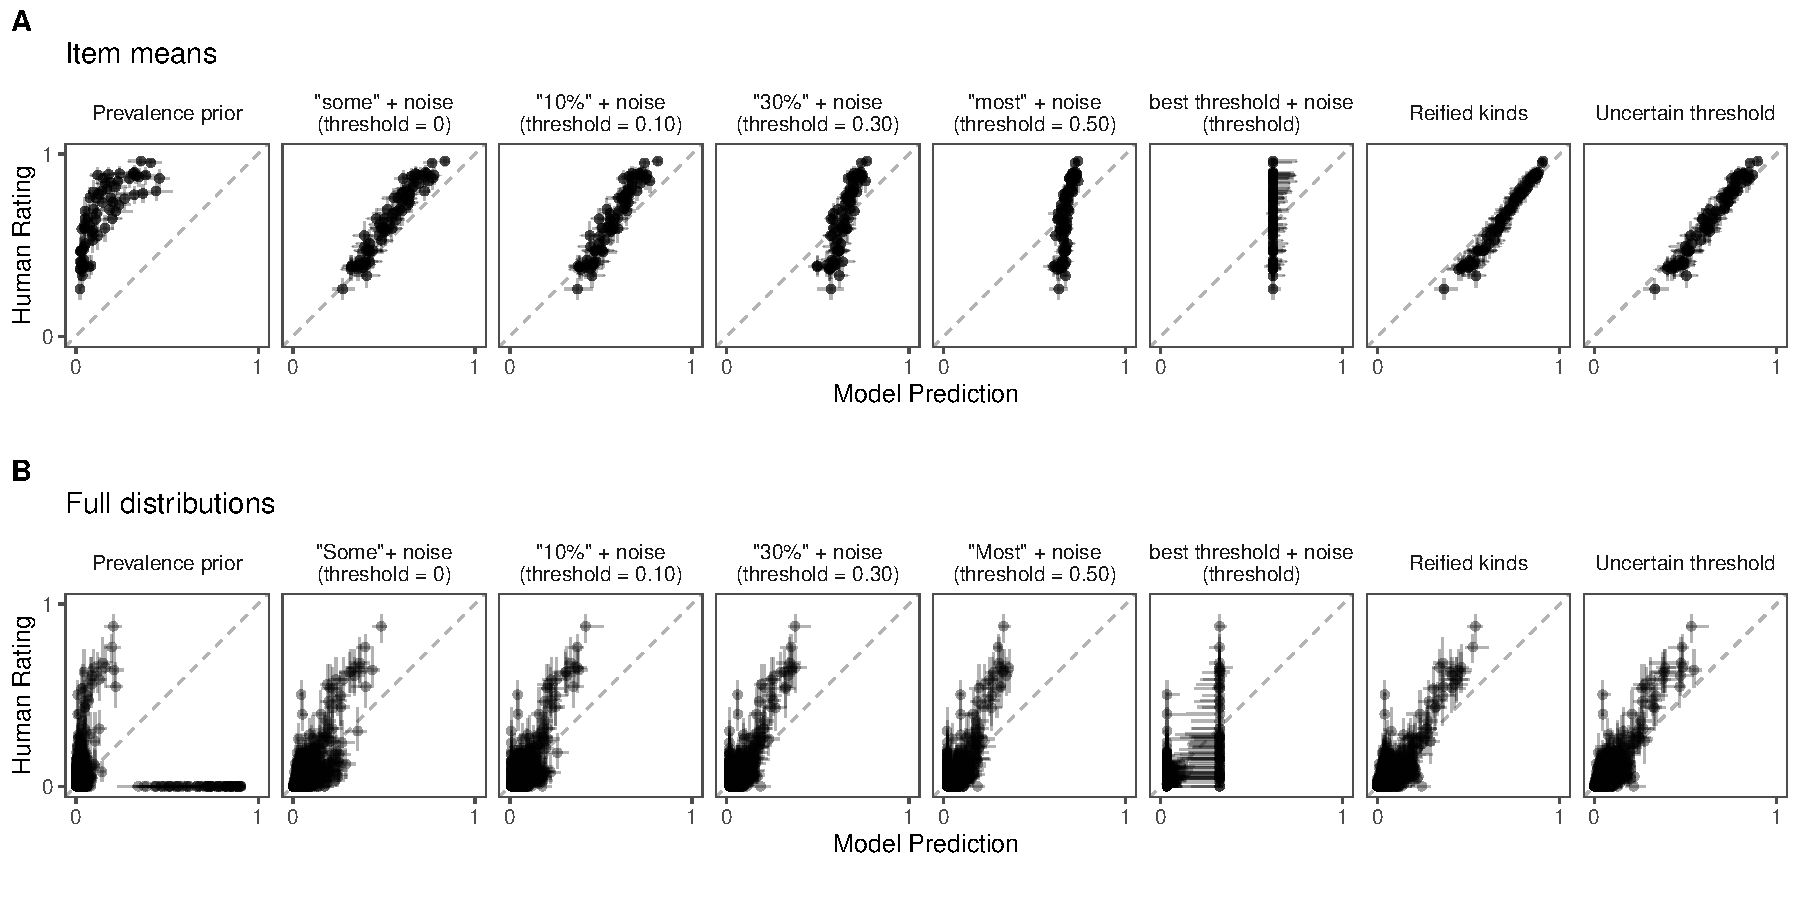
\includegraphics{figs/genint-modelingResults-plotgrid-scatters.pdf}
\caption{\label{fig:genint-modelingResults}Posterior predictive model fits for eight models in terms of their fit for (A) item means and (B) full distribution of responses for each individual item. Full distribution plots are created by discretizing the distributions to bins of width 0.05 (20 bins per item). Models are (from left to right): (i) the mean of the prevalence prior, (ii - v) a threshold semantics fixed at 0.01 (\enquote{some}), 0.1, 0.3, and 0.5 (``most''), (vi) a threshold semantics with a threshold inferred from the data (``best threshold''), (vii) the ``reified kinds'' model that picks out the component of the prior distribution with a higher mean, and (viii) the uncertain threshold model. Fixed-threshold models are outfitted with a noise parameter to accommodate data points that are logically impossible given the fixed semantics. Error bars denote bootstrapped 95\% confidence intervals for the behavioral data and 95\% highest posterior density intervals for the model predictions.}
\end{figure}

\hypertarget{model-criticism}{%
\paragraph{Model results}\label{model-criticism}}
%A qualitative examination of the inferred prevalence prior distributions showed that they were well-modeled as a mixture of two Beta distributions.
%Often one Beta distribution is devoted to accounting for the very small numbers (0\% or near 0\% prevalence ratings, for all the categories for which the property is absent), while the two other components account for the other parts of the distribution of responses, the details of which depend upon the property (see Figure~\ref{fig:genInt-prevPrior} for examples of priors of different shapes).
%To provide a quantitative examination of the fit to the priors data, we look at the posterior predictive distribution discretized to bins in increments of 10\% prevalence (i.e., categorical distributions over the bins of 0\%, 10\%, \ldots{}, 90\%, 100\% prevalence) and compare the model's inferred priors to the empirical counts that fell into those bins in the prior elicitation task.
%The joint data analysis model accommodates the empirical patterns in the prevalence priors very well: \(r^2(825) = 0.99\), \(MSE = 0.00052\).
%This indicates both that the mixture-of-Betas form is appropriate for the prevalence priors data and that the joint data analysis does not need to distort the prevalence priors in order to fit the generic interpretation data.
%
Overall, we find extremely strong evidence that the best model for how generics update beliefs is via an uncertain threshold semantics. 
The uncertain threshold model is many orders of magnitude better at jointly accounting for the data from the generic interpretation and prior elicitation tasks than any other model (Table \ref{tab:summary1}, log BF). 

% Finally, we ask whether one model is in fact a better explanation of the data using a formal model comparison technique.
%given the better fit of the pragmatic model but fewer parameters of the literal one, %Our second data analytic strategy is a formal model comparison to determine the extent to which the pragmatic generic interpretation model is the best explanation of the data, given it is a slightly more complex model than the literal interpretation model.

To gain deeper insight into why the uncertain threshold model is so much better than the alternative models, we examine each model's posterior predictive distribution of responses for each item. The posterior predictive distribution encodes the model's best guesses about what the data should look like, given the model and the parameters inferred from the data. 
We examine the posterior predictive distribution in two forms: (1) the expected value (or, mean) of the predicted responses for each item, and (2) the full distribution of responses for each item. In order to calculate summary statistics concerned the full distribution of responses, we discretize the model's predicted distribution and the empirical data to 20 equally spaced bins (bin-width = 0.05 on the 0-1 scale). 
With these comparisons, we find that the uncertain threshold model explains roughly 96\% of the variance in the mean data and about 71\% of the variance in the full distributions, with a very small mean squared error in comparison to the alternatives (Table \ref{tab:summary1}). 

%To evaluate how well each model can accommodate the implied prevalence data, we compare the item means for each of the 75 items to the the Maximum A-Posteriori (MAP) value of the expected value of each model's posterior predictive distribution . 
As a sanity check, we see that the model that predicts the implied prevalence ratings based only on the prevalence prior (\emph{Prevalence Prior}) does a poor job at predicting the mean human ratings (MSE = 0.27, $r^2 = 0.61$), with the model predicting lower prevalence values than participants report, consistent with the generic updating a listener's prior beliefs into stronger posterior beliefs (Figure \ref{fig:genint-modelingResults}A). 
Fixed threshold models exhibit an interesting inability to account for the mean implied prevalence ratings. The lowest threshold (0\% [``some'']) shows a strong correlation with the data, but like the Prior Prevalence model, predicts prevalence ratings that are too low relative to the human data, consistent with the intuition that assigning the semantics of \emph{some} for generics is too weak.
As the threshold value increases, the fixed-threshold models predict higher levels of implied prevalence, leading to model predictions that are too strong for certain generics (model prediction $>>$ human rating); this too-strong interpretation, in turn, leads the data analysis model to infer higher levels of noise as the threshold increases (MAP estimate of noise shown in Table \ref{tab:summary1}). 
This relationship between threshold and noise is most dramatically exemplified by the ``best threshold'' model, in which both threshold and noise are inferred from the data: this model ends up deciding that the threshold should be very high (MAP estimate = 0.93) as should the amount of noise (MAP estimate = 0.71), resulting in predictions that do not vary considerably by-item. 
Visually, this relationship between threshold value and noise results in a rotation of the model prediction line; as more responses must be attributed to noise, the model~vs.~data line appears more like a vertical line  (Figure \ref{fig:genint-modelingResults-bars}). 

\begin{figure}
\centering
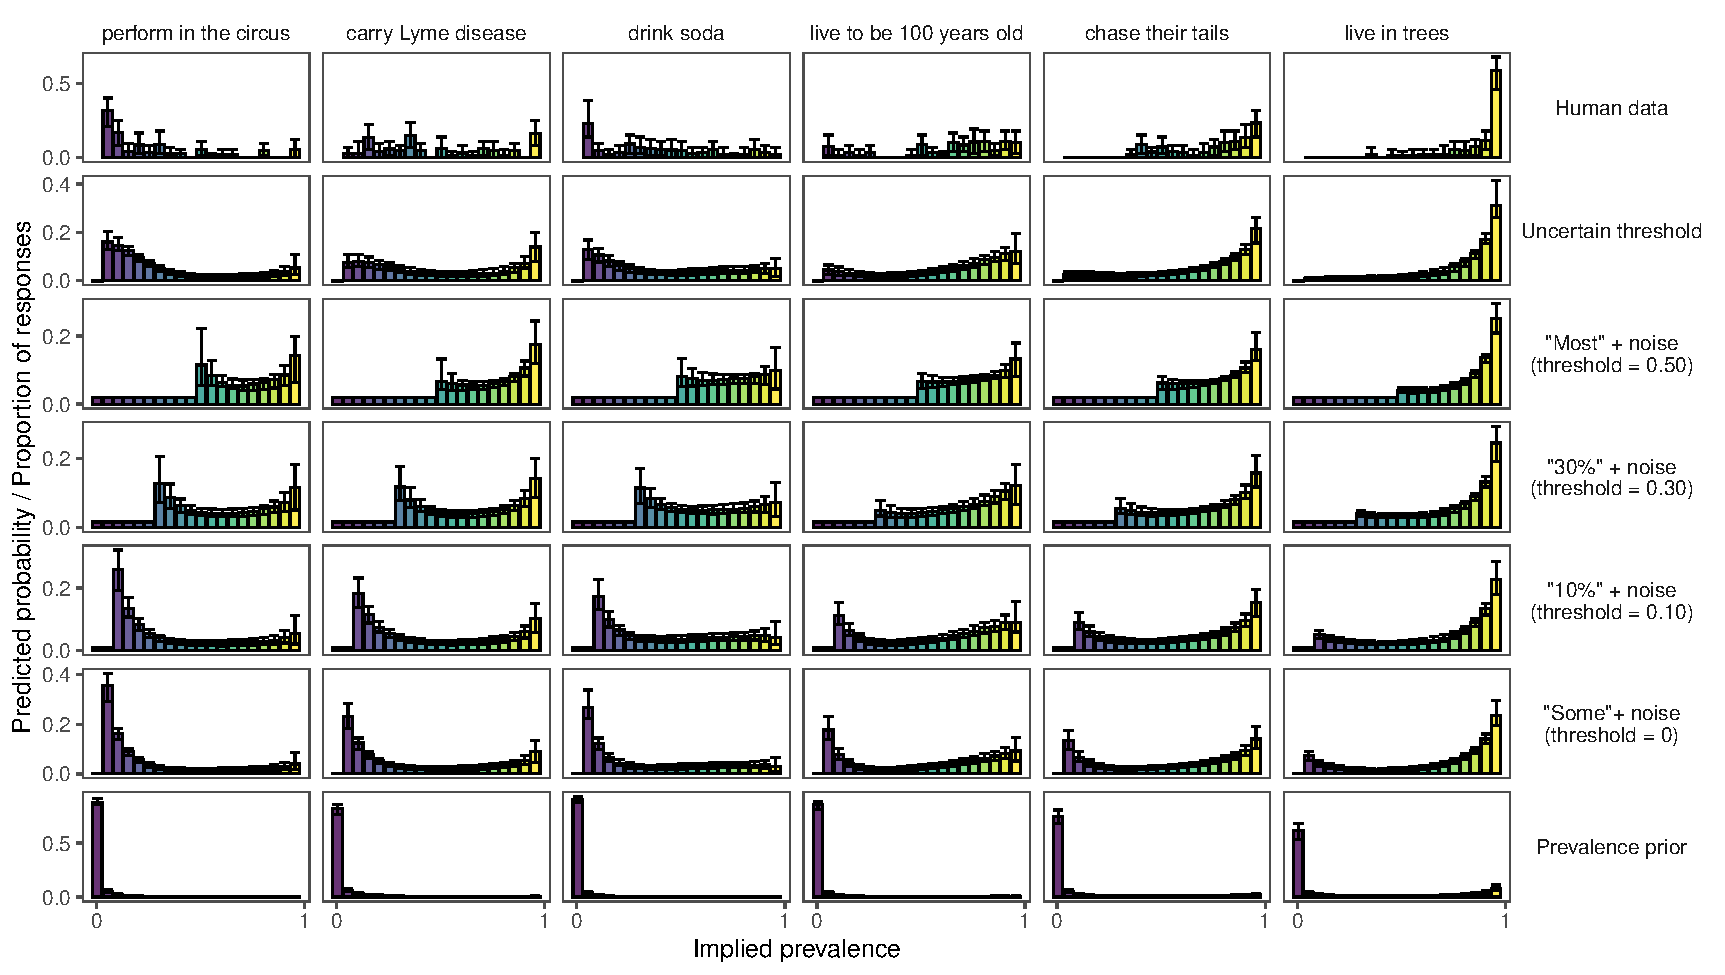
\includegraphics{figs/genint-fullDistributions-variousFixeds-1.pdf}
\caption{Distributions of implied prevalence ratings and model predicted distributions of responses for six items that span the spectrum of prevalence ratings. Individual fixed-thresholds capture the item distributions for certain items, but only the uncertain threshold captures all of the key features of the distributions for all of these items. The Reified kinds model closely tracks the Uncertain threshold model predictions, but comes apart for items where a multimodal distribution of interpretations is predicted (e.g., \emph{carry Lyme disease}).
}
\label{fig:genint-modelingResults-bars}
\end{figure}

The control model that performs the best is the \emph{Reified kinds} model, which predicts prevalence ratings based on a categorical (as opposed to continuous) view of the prevalence prior. This model selects the component of the prevalence prior distribution that has the highest mean and uses that to make predictions for generic interpretations (in the case of our 2-component prevalence prior, this model simply selects the component with the higher mean prevalence). 
This model seems to struggle the most with the ``weak generics'', the statements that receive overall low prevalence interpretations (Figure \ref{fig:genint-modelingResults}A; ``Reified kinds'', items below $y = x$ line).
By comparing the distribution of responses for \emph{Reified kinds}~vs.~\emph{Uncertain threshold}, we can see that  \emph{Reified kinds} fails to predict certain bi-modalities that the \emph{Uncertain threshold} model predicts.
For example, the statement \emph{Feps carry Lyme disease} is interpreted by some participants to mean that most or all feps carry Lyme disease, while others interpret it more weakly (some or few feps carry Lyme disease; Figure \ref{fig:genint-modelingResults-bars}). 
The \emph{Reified kinds} model partitions the prevalence prior into two distinct components and always selects the one with higher mean prevalence, thus only predicting the interpretation that most or all feps carry Lyme disease. 
By contrast, the \emph{Uncertain threshold} model treats the prevalence prior distribution as a continuous representation of belief about prevalence and is able to predict the bimodal interpretation. 
Overall, the \emph{Uncertain threshold} model is able to predict key signatures of full distributions of behavioral data, which no other model is able to adequately describe (Figure \ref{fig:genint-modelingResults}B).


%The strength of the uncertain threshold model can further by seen by examining the model's full distribution of responses on a by-item basis, rather than just the item means.
%For example, the item \emph{Ks carry Lyme disease} exhibits a high entropy empirical distribution: Participants (as a collective) are highly uncertain as to prevalence implied by the statement; it is possible that very few of the kind carries Lyme disease, and it is possible that almost all do as well. 
%The uncertain threshold model captures this diversity in responses, similar to the ``Some'' model in this case. 
%For other items, however, ``Some'' is too weak: For example, for \emph{Ks chase their tails}, the most compelling fixed-threshold model would the ``Most'' model, since responses for this item are predominantly above 50\%. 
%The uncertain threshold thus takes on the interpretations of different fixed-threshold models depending on the item, but this is not a variable that is stipulated in the model. 
%The model infers what is the best threshold by reasoning a variety of thresholds and taking into the prior distribution on prevalence. 


%Table \ref{tab:summary1} shows the mean squared errors and proportion of explained variance for predictions from models based on the prevalence prior alone, the uncertain threshold model, and fixed-threshold models for five values of the fixed-threshold (0\% [``some''], 10\%, 30\%, 50\% [``most''], and the best threshold models).
%All models show some correlation to the observed data, because all models encode informative prior beliefs about the property (Table \ref{tab:summary1}). 
%Figure~\ref{fig:genint-modelingResults}, however, reveals that both the prior only model and the belief-updating model based on the quantifier \emph{some} (i.e., a fixed threshold at the lowest possible value) consistently \emph{underpredict} the implied prevalence, consistent with the intuition that assigning the semantics of \emph{some} for generics is too weak.
%Increasing the threshold value for the fixed-threshold models leads the model to draw stronger interpretations from all generics, leading the model to \emph{overpredict} interpretations of weak generics,  which in turn causes the Bayesian data analysis model to infer higher values for the model's noise parameter (Table \ref{tab:summary1}).
%As the fixed-threshold increases, thus, so does the inferred amount of noise, which causes these models to wash away the differences in predictions between items (Figure~\ref{fig:genint-modelingResults}).
%The ``best'' threshold model, which treats the fixed-threshold as a free parameter inferred from the data, ends up deciding that the threshold should be very high (MAP estimate = 0.93) as should the amount of noise (MAP estimate = 0.71). 


%\begin{center}
%  \begin{table}[h]
%    \centering
%
%    \pgfplotstabletypeset[sci zerofill,
%    col sep = comma,
%    every head row/.style={before row = \toprule, after row = \midrule},
%    every last row/.style={after row = \bottomrule},
%    columns/semantics/.style={string type, column name={Fixed threshold}, column type = l},
%    columns/noise/.style={string type, column name={Inferred noise level}, column type = l}%,
%%    columns/Estimate/.style={column name={Estimate}, dec sep align},
%%    columns/Std. Error/.style={column name={SDE}, sci sep align, sci},
%%    columns/t value/.style={column name={$t$-value}, dec sep align},
%%    columns/Pr(>|t|)/.style={column name={$p$-value}, dec sep align }
%    ]
%    {csv_to_tex/expt1_model_param-posteriors.csv}
%
%    \caption{Inferred noise levels for fixed-threshold models with different values for the thresholds. Values reported are the Maximum A-Posteriori (MAP) estimates and 95\% Highest Posterior Density intervals.}
%    \label{tab:noise}
%  \end{table}
%\end{center}

 
%Though the model based on a semantics for \enquote{most} (i.e., a fixed threshold at 0.5) does better in terms of mean squared error, it explains substantially less variance; the \enquote{most} model attributes over the half of the data to noise (posterior MAP and 95\% credible interval for noise parameter $\omega = 0.57 {[}0.55, 0.59{]}$), because of the high number of responses below 50\%.

%Unlike each of the alternative semantic models, the two models based on belief updating according to an unspecified threshold (literal and pragmatic generics models) can accommodate the highly variable generic interpretation data with a high degree of quantitative accuracy.
%The pragmatic model slightly outperforms the literal generics model in terms of both mean squared error and variance explained at the level of average responses.
%The inferred values of the speaker optimality parameter \(\alpha\) was 2.03 {[}1.82, 2.18{]} and the generic cost parameter \(c\) was 3.6 {[}3.16, 4.27{]}.
%\mht{update with results from new model runs}





%Here, the empirical distribution it still 
%Figure~\ref{fig:genint-modelingResults-bars} shows these predicted distributions for seven example items covering the range of average responses from roughly 30\% implied prevalence to almost 100\%.

%All models exhibit some sensitivity to the variance in implied prevalence ratings, because they all use the prevalence prior in their definition.
%It is the actual magnitude of the strength of the generalization implied by the utterance that is predicted to be different, with the prior and \enquote{some} models predicting too weak of an interpretation.
%\enquote{Most} is handicapped by its high inferred rate of noise and does not make dramatically different predictions across the items.
%Both the literal and pragmatic generic interpretation models track the quantitative variance across these items.
%The evidence for pragmatic interpretations is most apparent for items that receive high but not at-ceiling implied prevalence ratings (e.g., \emph{have spots}, \emph{hunt other animals}; Figure~\ref{fig:genint-litPrag-scatter}).

%This result suggests that interpretations are most in dangerous of being strengthened beyond a speaker's intent for properties for which the listener is most uncertain about their distribution (cf., the asymmetry reported in Cimpian et al., 2010).\ndg{that last sentence (pointing to assymetry) needs to either be explained a lot more or cut.}

%{\textcolor{Blue}{[mht: could do a regression comparing whether or not the pragmatic model is better than the literal model (or the difference in sq.err) vs. the entropy of the prior... to see if pragmatics is most visible under conditions of uncertainty]}}\ndg{meh, i don't think it's needed...}




\begin{center}
  \begin{table}[h]
    \centering
    \small
    \pgfplotstabletypeset[fixed zerofill, precision = 2,
    col sep = comma,
    every head row/.style={before row = \toprule, after row = \midrule},
    every last row/.style={after row = \bottomrule},
    columns/semantics/.style={string type, column name={Model}, column type = l},
     columns/threshold/.style={string type, column name={Threshold}, column type = l},
          columns/noise/.style={string type, column name={Noise}, column type = l},
    columns/MSE/.style={column name={MSE}, fixed relative, dec sep, precision = 2},
      columns/r2/.style={column name={$r^2$}, dec sep},
    columns/r2_dist/.style={column name={$r^2_{dist}$}, dec sep},
     columns/mse_dist/.style={column name={$\text{MSE}_{dist}$}, fixed relative, dec sep, precision = 1},
    columns/log_bf/.style={column name={(log) BF}, dec sep, fixed, precision=0}%,
    ]
    {csv_to_tex/expt1_model_summary_stats2.csv}

    \caption{Summary statistics and parameters for models of generic interpretation. Threshold value for \emph{Best fixed-threshold} model is the MAP estimate inferred from the data; noise values are also MAP estimates inferred from the data. Mean Squared Errors and variance explained are calculated both at the level of the item means and over the distribution over responses discretized to bins of width 0.05 ($r^2_{dist}, \text{MSE}_{dist}$) for the generic interpretation data (Expt.~1b). Bayes Factors quantify evidence in support of each model relative to the Uncertain threshold model (in log scale) and are computed over the full distribution of responses for both the prior elicitation and generic interpretation tasks (Expts.~1a \& 1b). log BF values below 0 indicate evidence in support of the Uncertain threshold model.}
    \label{tab:summary1}
  \end{table}
\end{center}



%\begin{figure}
%\centering 
%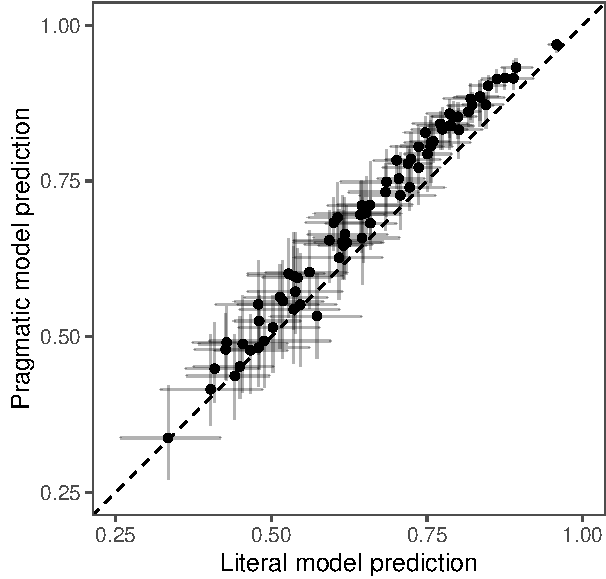
\includegraphics[width=0.4\textwidth]{genint_files/figure-latex/genint-litPrag-scatter-1} 
%\caption{Comparison of implied prevalence predictions for the literal~vs.~pragmatic generic interpretation models. The pragmatic model shows stronger interpretations for items that have intermediate implied prevalence. \mht{draw smoothed line to show the area under curve?}}
%\label{fig:genint-litPrag-scatter}
%\end{figure}




\hypertarget{preliminary-study-replication-and-extension-of-cimpian-et-al.-2010}{%
\section{Experiment 2: Replication and Extension of Cimpian et al. (2010)}\label{preliminary-study-replication-and-extension-of-cimpian-et-al.-2010}}

We use the same model based approach to re-examine the findings of Cimpian et al. (2010). As before, we measure the prevalence priors (Expt.~2a) and use those in combination with the models to predict the generic interpretation data (Expt.~2b), which is a replication and extension of the Cimpian et al. (2010) task. 

\subsection{Experiment 2a: Prior elicitation}

We take advantage of the finding in Expt.~1a that the prevalence priors elicited by asking about alternative categories were best modeled as a mixture of two Beta component distributions. 
We imagine one component governs the creatures that have some causal mechanism that stably gives rise to the property, while the other component is a null distribution, describing those creatures for which the feature could only be generated by an unstable, transient cause. 
Our prior elicitation task is then a structured task, where we ask about particular parameters of this model of the prevalence prior, and use Bayesian data analysis to reconstruct the prevalence priors implied by participants' responses. 


\subsubsection{Method}\label{method}

\paragraph{Participants}
We recruited 40 participants over Amazon's crowd-sourcing platform
Mechanical Turk (MTurk). We chose this number of participants based on
intuition from similar experiments which were designed primarily to test
a quantitative model. Participants were restricted to those with US IP
addresses and with at least a 95\% MTurk work approval rating. All
participants were native English speakers. The experiment took about 5-7
minutes and participants were compensated \$0.75.

\paragraph{Procedure}
Direct elicitation of background knowledge about the properties used in Cimpian et al. (2010) (e.g., by asking about prevalence in familiar
categories as did in Expt.~1a) is difficult because many of the properties are fantastical or obscure (e.g., pink teeth, silver legs, fungus-covered fur) which almost no familiar animals categories possess. 
Therefore,  we interrogate participants' latent beliefs about the property by assuming the mixture distribution validated in Expt.~1a -- where the prior is composed of a null distribution and a  \emph{stable cause} distribution -- and create an elicitation task to measure two aspects of the prior: (1) the relative contribution of the null distribution (e.g., for how many categories is the
property expected to be present at all) and (2) the shape of the stable cause distribution, the prevalence among
kinds where the property is present (\emph{prevalence when present}).

Participants were first introduced to a data-collection robot that was tasked with learning about properties of animals. Participants
were told the robot randomly selected an animal from its memory to ask
the participant about (e.g., The robot says: \enquote{We recently
discovered animals called feps.}). To measure the (inverse-) relative contribution
of the null prevalence distribution, the robot asked how likely it was
that there \emph{was a fep with the property} (e.g., \enquote{How likely is
it that there is a fep that has wings?}), to which participants reported
on a scale from \emph{unlikely} to \emph{likely}. To measure the shape of the stable cause distribution -- \emph{prevalence when present} -- the robot then asked the likely
prevalence assuming that at least an instance that had the property (e.g.,
\enquote{Suppose there is a fep that has wings. What percentage of feps
do you think have wings?}). Participants completed a practice trial
using the property \emph{is female} to make sure they understood the
meanings of these two questions. For example, it is very likely that
there is a fep that is female because almost all animals have female
members (high \(P(\text{feature is present})\)). Additionally, when
present, the property is only expected in about 50\% of the category.
Participants were provided corrective feedback if they did not answer the question within a range of valid responses.


\paragraph{Materials}
We constructed a stimulus set of forty different properties to explore a
wide range of \emph{a priori} beliefs about prevalence. These items make
up four categories of properties: body parts (e.g., \emph{fur}), body
parts of a particular color (e.g., \emph{yellow fur}), body parts
described with a vague adjective (e.g., \emph{curly fur}), and body
parts with in an accidental or disease state (e.g., \emph{wet fur}).
Pilot testing revealed more variability for items in the
accidental category relative to the other types of properties, and so we used
twice as many exemplars of accidental properties. We used eight exemplars of each of the three
non-accidental properties (parts, colored parts, vague parts), and
sixteen exemplars of accidental properties, building on the stimulus set
from Cimpian et al. (2010). List of properties is shown in Table B2 of
the Appendix.


\subsubsection{Data analysis and
results}\label{data-analysis-and-results}

Question 1 elicits the mixture parameter of a two-component mixture
model: \(P(\text{feature is present})\). Question 2 elicits the
prevalence in a kind where the property is present -- a sample from one component of the distribution. These elicited
parameters of the priors display a range of possible values
Figure~\ref{fig:cimpian-prevPrior}A. Biological properties are likely to
be present and when present, are likely to be widespread (top right
corner of scatter plot). More specific properties (either using gradable
adjectives or color adjectives) are expected to be slightly less
prevalent among the kinds where the property is present, perhaps
reflecting the fact that the same kind of animal can come in many
different colors or sizes; in addition, gradable properties (e.g., \emph{big claws}) imply comparison classes (e.g., big for an X) which could further restrict the prevalence. Finally, accidental properties
are roughly equally as likely to be present in a category as the color or gradable
properties (same \(P(\text{feature is present})\)), but are not expected
to be as widespread when present in the category (low \emph{prevalence
when present}).

From these two elicitation questions, we can reconstruct the marginal distributions on prevalence, which we have been calling the prevalence priors.
We assume that kinds for which the
property is absent have prevalence levels sampled from a Beta
distribution that heavily favors numbers close to 0:
\(\text{Beta}(\gamma = 0.01; \xi = 100)\).\footnote{Note that we use the
  noncanonical mean \(\gamma\) and concentration \(\xi\) (or,
  inverse-variance) parameterization of the Beta distribution rather
  than the canonical shape (or pseudocount) parameterization for ease of
  posterior inference. The shape parameterization can be recovered
  using: \(\alpha = \gamma \cdot \xi; \beta = (1 - \gamma) \cdot \xi\).}
With that assumption, the marginal prior distribution on prevalence is given by:\footnote{All
  modeling results hold when this null distribution is assumed to be
  even more left-skewed \(\text{Beta}(\gamma = 0.001; \xi = 1000)\) or
  just a delta-function at zero \(\delta_{p=0}\).}

\begin{align}
\phi & \sim \text{Beta}(\gamma_1, \xi_1) \nonumber \\ 
r & \sim \begin{cases}
        \text{Beta}(\gamma_2, \xi_2) &\mbox{if } \text{Bernoulli}(\phi) = \textsc{T} \label{eq:priorModel}  \\
        \text{Beta}(\gamma = 0.01; \xi = 100) &\mbox{if } \text{Bernoulli}(\phi) = \textsc{F} \\
        \end{cases}
\end{align}

For data analysis, we assume participants' responses to both questions
(\(i \in \{\text{Question 1}, \text{Question 2}\}\)) are generated from
Beta distributions: \(d_{i} \sim \text{Beta}(\gamma_i, \xi_i)\), and put
uninformative priors over the parameters of each:
\(\gamma_i \sim \text{Uniform}(0, 1); \xi_i \sim \text{Uniform}(0, 100)\).
%We implemented this Bayesian mixture-model in the probabilistic
%programming language WebPPL (Goodman \& Stuhlmüller, 2014). 
To learn
about the credible values of the parameters of the model, we ran MCMC on
each item independently for 100,000 iterations, discarding the first
50,000 for burn-in.

Figure~\ref{fig:cimpian-prevPrior}B shows example reconstructed priors for eight properties.
Biological properties (\emph{biological}, \emph{vague}, and \emph{color}
body parts) have prevalence distributions that are bimodal with peaks at
0\% and near-100\% prevalence, but differ in their variance around the
100\%-mode. By contrast, accidental properties do not have a substantial
second mode. This variability in prevalence priors leads the generic
interpretation model to predict different prevalence levels implied by
the generic.

\begin{figure}
\centering
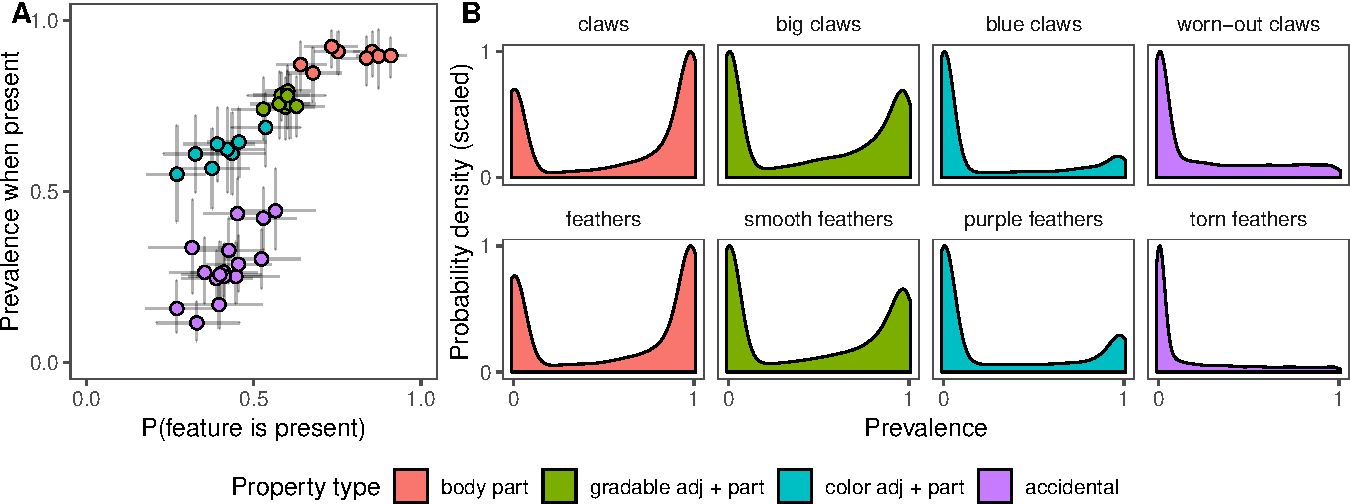
\includegraphics{genint_files/figure-latex/cimpian-prevPrior-1.pdf}
\caption{\label{fig:cimpian-prevPrior}Prevalence priors for items from
Cimpian et al. (2010). A: Latent parameters governing prevalence priors
are different for different kinds of properties. B: The diversity in
parameters gives rise to different underlying distributions over
prevalence, which the generic interpretation model uses to make
predictions.}
\end{figure}


\begin{figure}
\centering
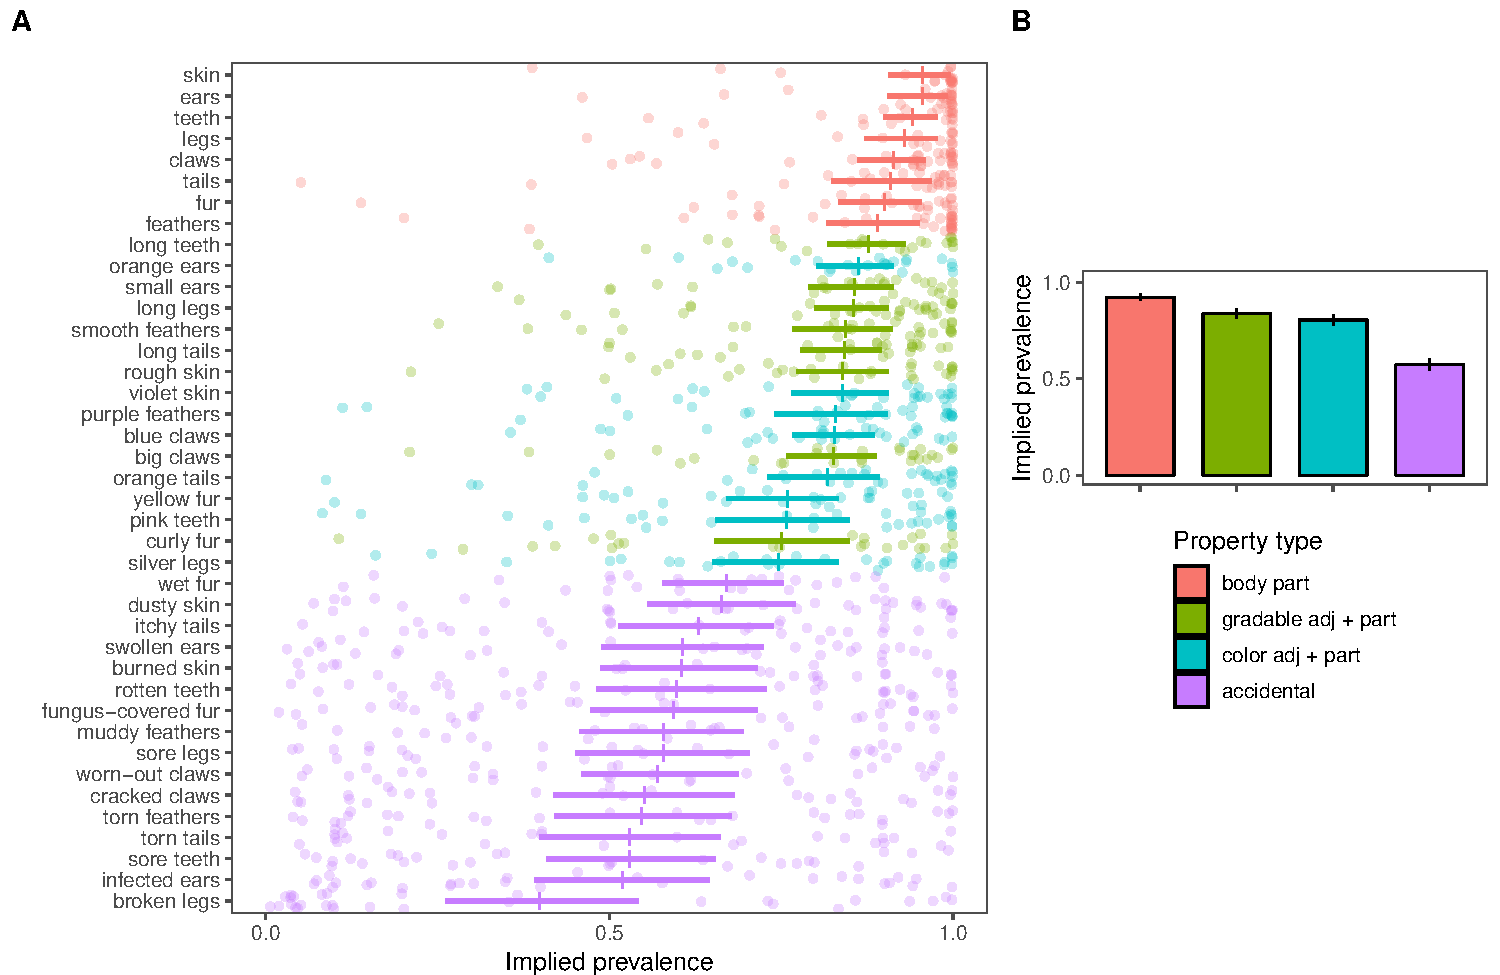
\includegraphics{figs/cimpian-results}
\caption{\label{fig:cimpian-modelingResults}Implied prevalence data for items from Cimpian et al. (2010). A: Implied prevalence ratings for forty body-part stimuli (\emph{Ks have F}). Vertical line denotes mean, horizontal lines denotes bootstrapped 95\% confidence intervals, points are individual responses. B: Implied prevalence collapsed across property type. The original result of Cimpian et al. (2010) showed a difference between \emph{color adj + part} and \emph{accidental}.}
\end{figure}

% As we did for Expt.~1, we implemented joint Bayesian data analysis models that predict the structured elicitation responses (Expt.~2a) and use the inferred prevalence priors to predict the generic interpretation data (Expt.~2b) assuming different models of generic interpretation (uncertain threshold, fixed-thresholds, reified kinds). 

\begin{figure}
\centering
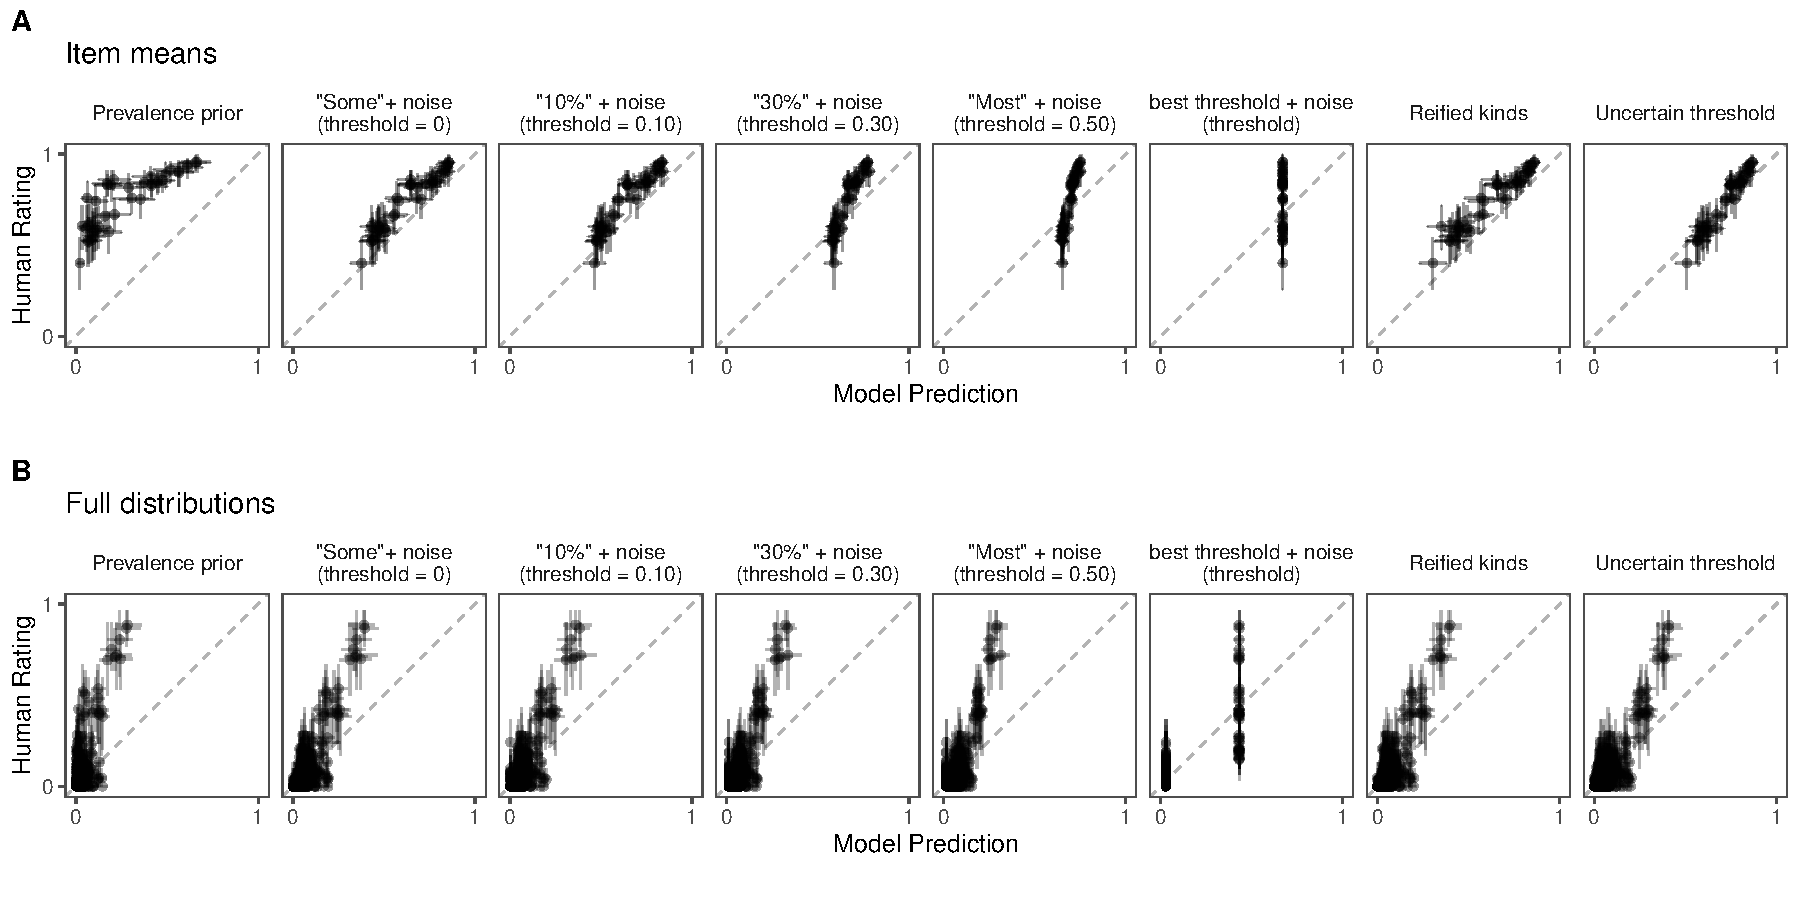
\includegraphics{figs/cimpian-modelingResults-plotgrid-scatters.pdf}
\caption{\label{fig:cimpian-modelingResults-scatters}Posterior predictive model fits for the Cimpian et al. (2010) replication data. (A) shows item means and (B) full distribution of responses for each individual item. Full distribution plots are created by discretizing the distributions to bins of width 0.05 (20 bins per item). Models are (from left to right): (i) the mean of the prevalence prior, (ii - v) a threshold semantics fixed at 0.01 (\enquote{some}), 0.1, 0.3, and 0.5 (``most''), (vi) a threshold semantics with a threshold inferred from the data (``best threshold''), (vii) the ``reified kinds'' model that picks out the component of the prior distribution with a higher mean, and (viii) the uncertain threshold model. Fixed-threshold models are outfitted with a noise parameter to accommodate data points that are logically impossible given the fixed semantics. Error bars denote bootstrapped 95\% confidence intervals for the behavioral data and 95\% highest posterior density intervals for the model predictions.}
\end{figure}


\begin{figure}
\centering
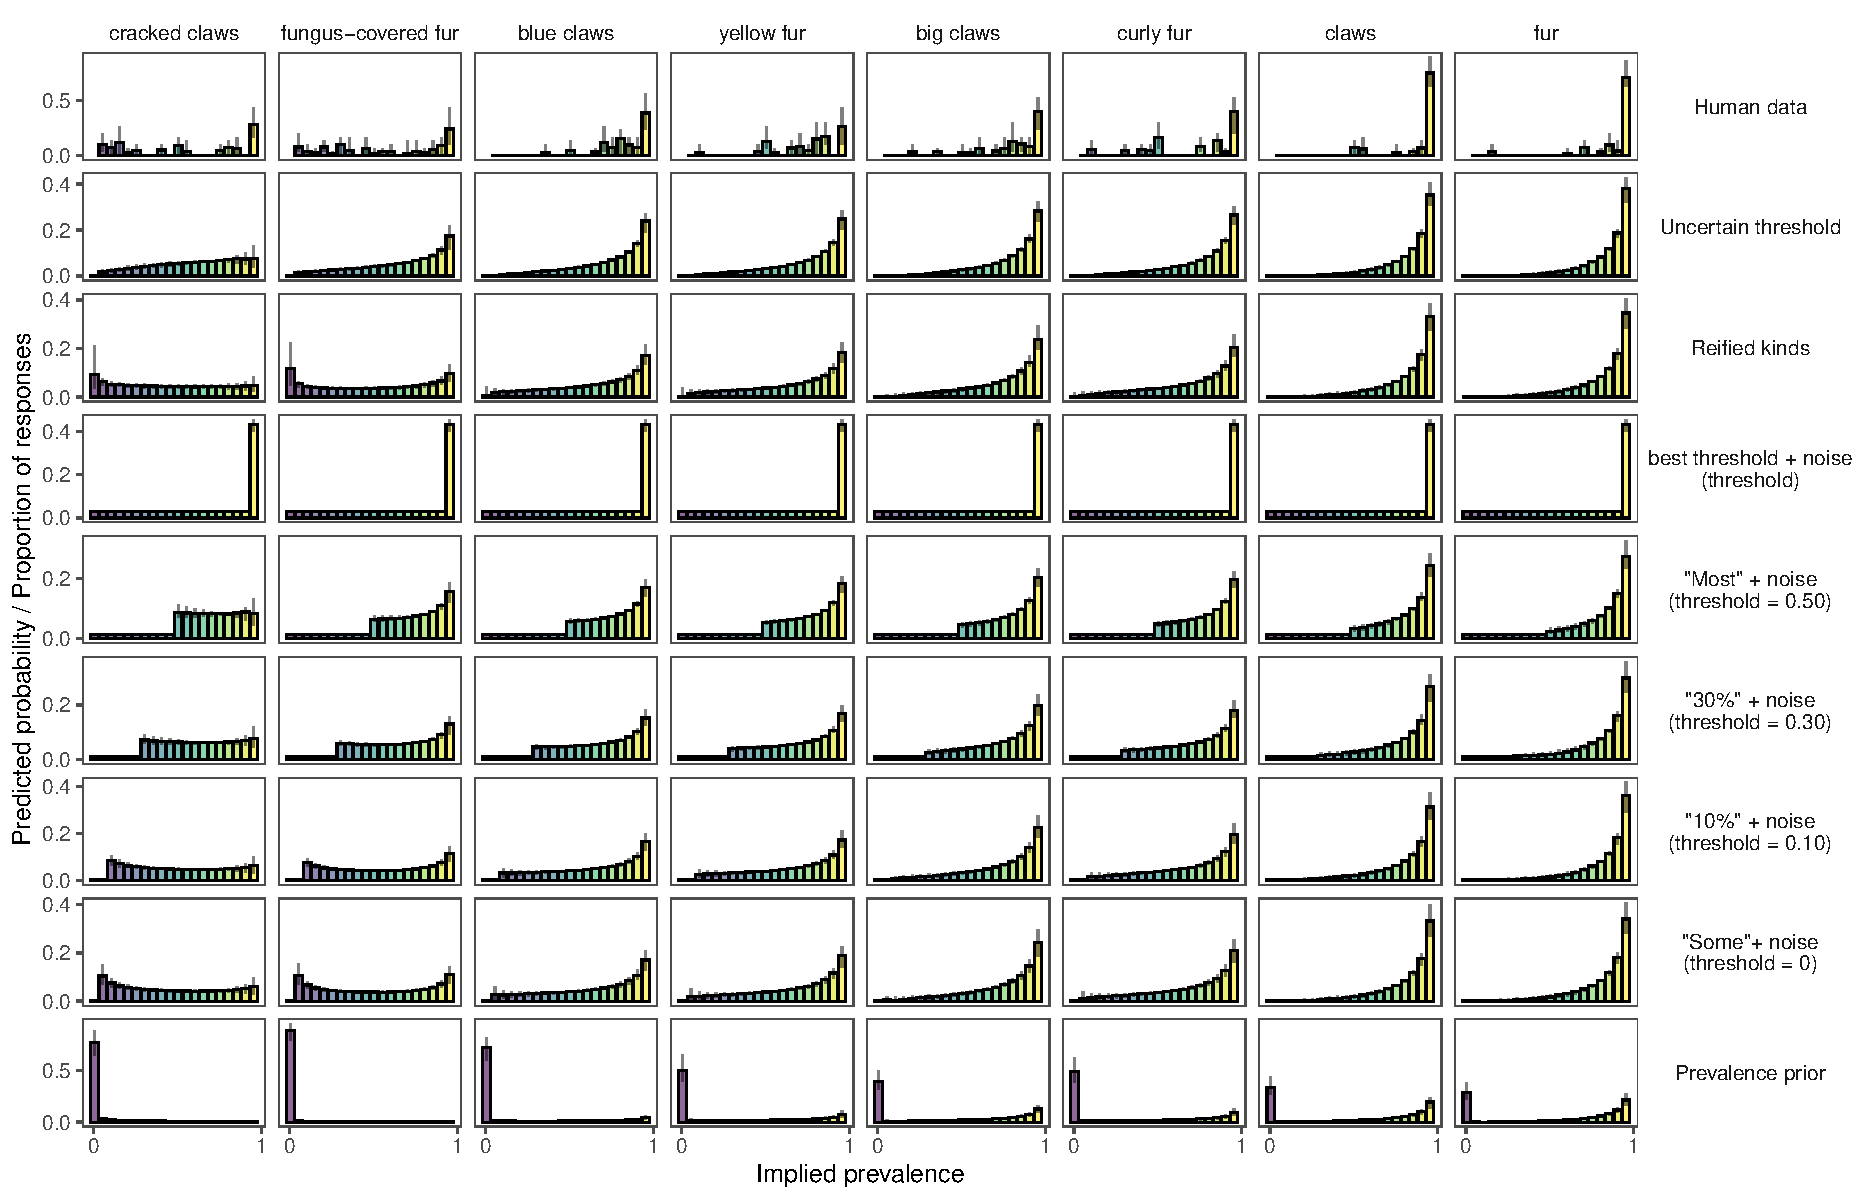
\includegraphics{figs/cimpian-fullDistributions-variousFixeds-1.pdf}
\caption{Distributions of implied prevalence ratings and model predicted distributions of responses for eight items from Expt.~2.
}
\label{fig:cimpian-modelingResults-bars}
\end{figure}


\subsection{Experiment 2b: Generic interpretation}

%\hypertarget{method}{%
\subsubsection{Method}\label{method}

\paragraph{Participants}
%\hypertarget{participants}{%
%\subsection{Participants, procedure, and materials}\label{participants}}
We recruited 40 participants over Amazon's crowd-sourcing platform Mechanical Turk.
The experimental design is very similar to \citeA{Cimpian2010}, and we chose to have a sample size at least twice as large as the original study (original n=15).
All participants were native English speakers.
The experiment took about 5 minutes and participants were compensated \$0.60.

%\hypertarget{procedure-and-materials}{%
%\subsubsection{Procedure and materials}\label{procedure-and-materials}}

\paragraph{Procedure and materials}
The materials were the same as in Expt.~2a.
Participants were told they were the resident zoologist of a team of scientists on a recently discovered island with many unknown animals and that their task was to provide their expert opinion on questions about these animals.
On each trial, participants were supplied with a bare plural sentence of the form \emph{Ks have F}, where K was a novel category label and F was a familiar property (e.g., \emph{Feps have yellow fur}; see Table B2 in Appendix for list of properties).
Participants were then asked to judge prevalence: \enquote{What percentage of feps do you think have yellow fur?}
Participants responded using a slider bar with endpoints labeled 0\% and 100\%, with the exact number corresponding to their slider bar rating displayed once participants clicked on the slider bar.
%\paragraph{Materials}
Participants completed in randomized order 25 trials: 5 for each of the biological properties and 10 for the accidental.
%Our stimulus set was comprised of 40 properties, which we divided into three sets of eight biological properties (body parts described with a color adjective e.g., \emph{purple feathers}, body parts described with a gradable adjective  e.g., \emph{long teeth}, and body parts with no adjective e.g., \emph{fur}) and one set of 16 body parts in accidental or diseased states (e.g., \emph{wet fur} or \emph{broken legs}).
%\ndg{need a sentence about the classes of properties and where the items come from... all are from cimpian, or we added some?}

\hypertarget{results-and-discussion}{%
\subsubsection{Results}\label{results-and-discussion}}

%Interpreting a novel generic sentence \emph{Ks F} often has the possibility of being understood as a universal or near-universal claim (\emph{all or almost all Ks F)}.
Across the forty items in this experiment, we observe a gradient in the implied prevalence ratings similar to that revealed by Expt.~1a. Here, the continuum is mostly clustered by the higher-order type of property (Figure~\ref{fig:cimpian-modelingResults}A).
At the level of property type, \citeA{Cimpian2010} found a difference between the implied prevalence of generics about biological parts described with color adjectives (e.g., \emph{purple feathers}) and accidental properties (e.g., \emph{fungus-covered claws}).
We replicate this result and extend it to show further gradability among types of properties (Figure~\ref{fig:cimpian-modelingResults}B) as well as within types.

 \citeA{Cimpian2010} noted that for the accidental property generics: \enquote{properties of this type do not lend themselves very well to generic predication \cite{gelman1988development, Cimpian2008}, so generics about broken legs, itchy skin, etc. are infrequent outside the laboratory.} (p.1472). It is possible that the order of presentation of the items could influence participants' judgments, with later trials providing more experience to the participant that they are dealing with generic statements.\footnote{We thank an anonymous reviewer for suggesting this look at the data.} Such an order effect could result in either (a) higher ratings in later trials, as participants impute high-prevalence generic interpretations on to the accidental property generics, rather than an existential reading of the statement or (b) lower ratings in the later trials, as participants get more experience with the variability in types of properties, they begin to realize that generics about different properties can be variable with respect to the prevalence they imply. Note that explanation (a) is confounded with typical regression-to-the-mean, as items that receive significantly lower-than-average responses early in the task will tend to receive relatively higher responses later in the task. We investigated this quantitatively by building a Bayesian mixed-effects regression model predicting the response as a function of the property type (biological vs. accidental vs. color vs. vague modifier), the half of the experiment in which the item was rated by the participant, and their interaction. The model additionally included random effects of intercept and effect of split-half by item and intercept, split-half, property type, and their interaction by participant (the maximal random effects structure). Consistent with explanation (b), we found that participant ratings were slightly higher in the first half than the second half for the accidental items (posterior mean and 95\% Bayesian Credible Intervals: $\beta = 0.06 [0.03, 0.10]$). No difference was observed between first half and second half ratings for the other property type conditions ($\beta_{color} = 0.02 [-0.03, 0.07]; \beta_{vague} = 0 [-0.05, 0.05], \beta_{part} = 0 [-0.04, 0.05]$).
 
To test our quantitative models in their ability to explain the data from Cimpian et al. (2010), we implemented joint Bayesian data analysis models that predict the structured elicitation responses (Expt.~2a) and use the inferred prevalence priors to predict the generic interpretation data (Expt.~2b) assuming different models of generic interpretation (uncertain threshold, fixed-thresholds, reified kinds) in a manner directly analogous to what we did for Expt.~1. 
The priors on parameters were the same as for the modeling of Expt.~1. 
To compute the posterior distribution over parameters and generate posterior predictive distributions, we ran for each model 3 MCMC chains consisting of $10^6$ iterations discarding the first $5 \times 10^5$ for burn-in, and checked convergence qualitatively by visual inspection of the parameters and predictions of each chain. 
We additionally performed a formal Bayesian model comparison by computing the marginal likelihood of the data under each model (in order to compute Bayes Factors); to do this, for each model, we collected 200 samples from an Annealed Importance Sampling algorithm with an annealing schedule consisting of 10,000 uniformly spaced increments. 

As we observed in Expt.~1a, the best fitting and most parsimonious model of the data from Cimpian et al. (2010) is the \emph{Uncertain threshold} model, explaining 96\% of the variance in the mean ratings by item in this data set (Table \ref{tab:cmpsummary}).
Both the \emph{some} model and the \emph{Reified kinds} model appear to perform similarly well for many items (Figure \ref{fig:cimpian-modelingResults-scatters}), but systematically predict too high of prevalence ratings for items across the scale. 
Once again, when the data analytic model is allowed to jointly infer the best fixed-threshold and best noise level, the model infers very high levels of noise, washing out any differences one observes across the items (Figure \ref{fig:cimpian-modelingResults-bars}).
The results show that the differences originally observed by Cimpian et al. (2010) can be accounted for quantitatively by an uncertain threshold model that operates over diverse prior beliefs about properties.

%To evaluate the uncertain threshold model as an explanation of the data (and in comparison to its its alternatives), we constructed a Bayesian data analysis model to jointly predict the prevalence prior data (Expt.~2a) and the generic interpretation data (Expt.~2b).
%As we did for Experiment 1, we model the prevalence prior data for each distribution condition as a mixture of two Beta distributions (with unknown means, variance, and mixture parameters) and we model the generic interpretation via the uncertain threshold model (or an alternative model) that assumes the prevalence prior inferred from the Expt.~2a data (Figure \ref{fig:bayesnet}).
%As before, fixed-threshold alternative models make an additional use of a noise parameter to accommodate data points that are literally incompatible with the model. 




%\mht{add brm results for prevalence $\sim$ property type ?}



\begin{center}
  \begin{table}[h]
    \centering
    \small
    \pgfplotstabletypeset[fixed zerofill, precision = 2,
    col sep = comma,
    every head row/.style={before row = \toprule, after row = \midrule},
    every last row/.style={after row = \bottomrule},
    columns/model_name/.style={string type, column name={Model}, column type = l},
    columns/MSE/.style={column name={MSE}, fixed relative, dec sep, precision = 2},
      columns/r2/.style={column name={$r^2$}, dec sep},
    columns/r2_dist/.style={column name={$r^2_{dist}$}, dec sep},
     columns/MSE_dist/.style={column name={$\text{MSE}_{dist}$}, fixed relative, dec sep, precision = 2},
    columns/log_bf/.style={column name={(log) BF}, dec sep, fixed, precision=0}%,
    ]
    {csv_to_tex/cmp_model_summary_stats.csv}
    \caption{Summary statistics of models for Expt.~2. Mean Squared Errors and variance explained are calculated both at the level of the item means and over the distribution over responses discretized to bins of width 0.05 ($r^2_{dist}, \text{MSE}_{dist}$) for the generic interpretation data (Expt.~2b). Bayes Factors quantify evidence in support of each model relative to the Uncertain threshold model (in log scale) and are computed over the full distribution of responses for both the prior elicitation and generic interpretation tasks (Expts.~2a \& 2b). The Best fixed-threshold model has no variance in its predictions about the item means. log BF values below 0 indicate evidence in support of the Uncertain threshold model.}
    \label{tab:cmpsummary}
  \end{table}
\end{center}

%Threshold value for \emph{Best fixed-threshold} model is the MAP estimate inferred from the data; noise values are also MAP estimates inferred from the data. 



%Broadly, these results validate the implied prevalence measurement as one that can elicit variability in interpretations, and it is this variability that is of primary concern to us.
%The items that elicited the most variability in implied prevalence ratings were those of accidental or diseased states (e.g., \emph{Lorches have broken legs}, \emph{Wugs have fungus-covered claws}).
%As \citeA{Cimpian2010} noted, \enquote{properties of this type do not lend themselves very well to generic predication \cite{gelman1988development, Cimpian2008}, so generics about broken legs, itchy skin, etc. are infrequent outside the laboratory.} (p.1472)
%Not only are these kinds of statements infrequent outside the laboratory, bare plurals about accidental or diseased states (\emph{Lorches have broken legs}) can easily be interpreted as non-generic, existential claims about the here-and-now, analogous to how \emph{Dogs are on my front lawn} describes a particular state of affairs as opposed to something generalizable about dogs.
%Since the strongest test of our models of generic interpretation will come from having to predict variability in implied prevalence ratings, we aim to elicit high variability in Experiment 2 using naturalistic properties that more easily lend themselves to generic predication.


%The development of induction within natural kind and artifact categories. Cognitive Psy- chology,




\hypertarget{experiment-3-prior-manipulation}{%
\section{Experiment 3: Prior Manipulation}\label{experiment-3-prior-manipulation}}

In our second experiment, we test the causal role of the prevalence prior in generic interpretation.
In the previous experiment, participants' prior beliefs about the prevalence of the property, measured by asking about alternative categories (Expt. 1a), related to the prevalence implied by a novel generic (Expt. 1b) via the uncertain threshold model.
Though the uncertain threshold model is able to finely track interpretations in a way that alternative models cannot, the evidence so far for the influence of the prevalence prior on interpretation is merely correlational.
Here we manipulate the prevalence prior and measure the resulting influence on interpretation.
To serve as a manipulation check, we first elicit predictions about prevalences following our prior manipulation procedure; these predictions also serve as the measurements of the (manipulated) prevalence priors used in our model.

\hypertarget{experiment-3a-prior-elicitation-manipulation-check}{%
\subsection{Experiment 3a: Prior elicitation (manipulation check)}\label{experiment-3a-prior-elicitation-manipulation-check}}

In this experiment, we elicit participants' beliefs about the prevalence of a property among different categories following a manipulation designed to alter participants' beliefs about a property.


\hypertarget{methods-2}{%
\subsubsection{Methods}\label{methods-2}}

\hypertarget{participants-3}{%
\paragraph{Participants}\label{participants-3}}
%
We recruited 450 participants from MTurk.
This number was arrived at with the intention of getting approximately 40 participants to provide ratings for each unique condition in the experiment, for an intended total of approximately 200 ratings per condition.\footnote{The intended number of ratings is larger than the corresponding number of ratings in Expt.~1a. We decided to increase the target number of ratings because we anticipated more noise in this task (as a result of it being a single trial experiment) and because we had fewer numbers of unique items or conditions in Expt.~3 than in Expt.~1.}
The experiment took on average 3 minutes and participants were compensated \$0.30.

\hypertarget{materials-1}{%
\paragraph{Materials}\label{materials-1}}
%
The goal of this experiment was to manipulate the prevalence prior.
Participants were familiarized with one of ten prevalence prior distributions, shown in Figure~\ref{fig:priorManipulationExpt}E.
In Experiment 1a, we found that the prevalence priors for familiar properties were best-modeled as a mixture of two Beta distributions.
Hence, in these experiments, nine of our ten distribution were bimodal, with modes either at 0\%, 25\%, 50\%, 75\%, or 100\%; the tenth distribution was uniform over all prevalence levels between 0\% and 100\%.
For the bimodal distributions, the mixture between the two modes was always 50\% (half of samples were from one mode and half from the other, as shown in Figure~\ref{fig:priorManipulationExpt}B).

%\mht{}
Our cover story involved learning about a single property, so that we could assign credit of differences in interpretations back to the manipulated prior distribution, rather than knowledge about properties (which we studied in Experiment 1). 
Pilot testing revealed that using a completely novel property (e.g., \emph{daxing}) made our task highly artificial. 
Thus, we used a property from Experiment 1 that we though would be particularly amenable to manipulation by selecting a property whose prevalence prior had high entropy (i.e., participants had lots of uncertainty as to what prevalence levels to expect for this property); the property we used was the predicate \emph{know when earthquakes are about to happen}.

\hypertarget{procedure}{%
\paragraph{Procedure}\label{procedure}}
%
\begin{figure}
\centering
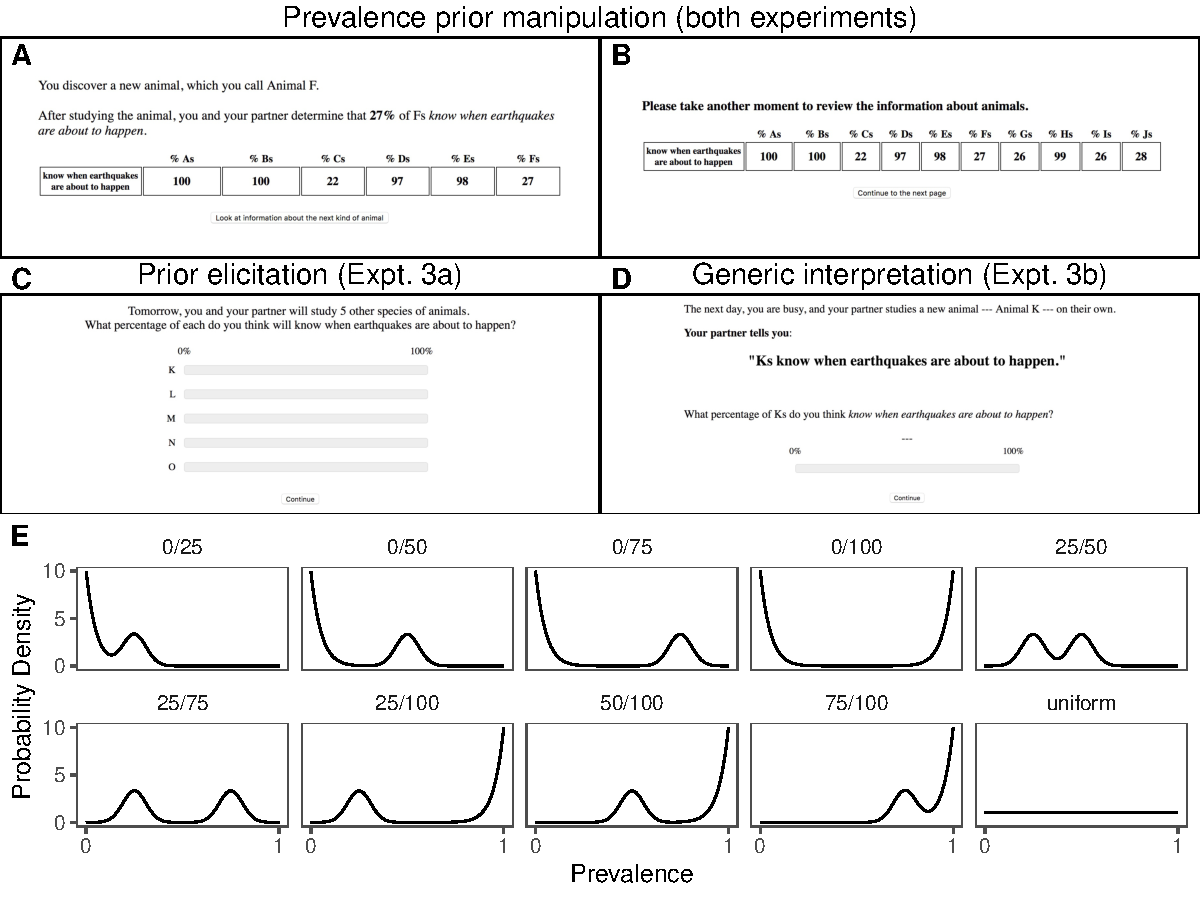
\includegraphics{figs/expt2-overview.pdf}
\caption{\label{fig:priorManipulationExpt}Overview of Experiment 2. A: Prevalences of feature in animals are shown one at a time, described in text and displayed in a table. B: Participants are asked to review previous results once all displayed. C: Prior elicitation task: Participants predict the results of the next five animals. D: Generic interpretation task: Participants rate prevalence after reading generic sentence. E: Experimentally manipulated prevalence prior distributions. The distribution shown in B is the \emph{25/100} distribution.}
\end{figure}
%
In order to avoid participants learning and reasoning about the structure of the task, participants completed only a single trial: Each participant saw only one prevalence distribution.
Participants were given a cover story in which they were asked to imagine they were an astronaut-scientist exploring a distant planet with many new animals on it.
They were studying these animals with another scientist to understand the animals' ability to \enquote{know when earthquakes are about to happen}.
Participants were then shown data that they and their fellow scientist had collected about the prevalence of the property among different novel animals.
In order to minimize distraction, novel animals were simply labeled by a letter (e.g., \enquote{Animal C} or just \enquote{Cs}).
Information about the animal appeared in an \emph{evidence statement} (e.g., \enquote{After studying the animal, you and your partner determine that 98\% of Cs \emph{know when earthquakes are about to happen}.}) and was displayed in a table showing the corresponding numerical data (Figure~\ref{fig:priorManipulationExpt}A).
Participants proceeded in a self-paced way by clicking a button to reveal information about the next animal.
After participants viewed the data for ten categories, they are told to review the information about the animals before continuing (Figure~\ref{fig:priorManipulationExpt}B).
Then, the data table was removed and participants were provided the following prompt:

\begin{quote}
Tomorrow, you and your partner will study 5 other new species of animals. What percentage of each do you think will know when earthquakes are about to happen?
\end{quote}

Participants were given five slider bars ranging from 0\% - 100\%, and asked to predict the prevalence for the next five categories (Animals K - P; Figure~\ref{fig:priorManipulationExpt}C).
After rating the slider bars, we asked participants to explain why they gave the responses that they did.
Then, they completed an attention check survey where they were asked what property was being investigated (choosing a response from a list of 10 options) and to input one of the prevalence levels they saw on the familiarization screen.

\hypertarget{results-1}{%
\subsubsection{Results}\label{results-1}}

Participants who failed to either select the correct property or list a correct number from the familiarization period were excluded ($n=26$), in addition to participants who reported a native language other than English ($n=24$), leaving a total of $n=403$ participants whose data we analyzed.
Similar to the data from Expt. 1a, a response in this task can be thought of as a sample from a prevalence prior distribution and the distribution of responses as estimates for the whole distribution.
We visualize the distributions by discretizing the responses so that each response goes into one of twenty equally spaced bins (effectively turning the 101-pt scale into a 20-pt scale).
Figure~\ref{fig:genint-modelingResults2}A (top row) shows the empirically elicited predicted prevalence distributions.
These distributions clearly reflect the familiarization distributions supplied to participants in the experiment, indicating a successful manipulation, with some idiosyncratic features.
The distribution that is most different from the familiarization distribution is the uniform distribution; the empirical distribution is more unimodal with a peak at 50\%.
Many distributions exhibit a regression to the mean in some participants' predictions: In the \emph{rare or deterministic} distribution (which featured prevalence levels either around 0\% or 100\%), some participants guess that the next animal will have 50\% prevalence; a similar phenomenon can be observed in the \emph{weak or strong} distribution (25\% or 75\%) and to a lesser extent in the other bimodal distributions.



\hypertarget{experiment-2b-generic-interpretation}{%
\subsection{Experiment 2b: Generic interpretation}\label{experiment-2b-generic-interpretation}}

In this experiment, we measure participants' interpretations of generic statements about novel categories following the same manipulation of Expt.~2a, whited altered participants' beliefs about the prevalence of a property among different categories (i.e., the prevalence prior). 


%We use the empirically measured prevalence distributions from Expt. 2a to generate \emph{a priori} model predictions about the generic interpretation data from our five models.\footnote{For the pragmatic model, we fix the two parameters to be the maximum a-posteriori inferred values from the Expt. 1 analysis: \(\alpha = 2; c = 3.5\).}
%To account for our uncertainty in the measurement of the prevalence priors, we bootstrap the priors by resampling subjects (with replacement), calculating the empirical prevalence distributions (by binning, as above), and generating model predictions.
%We repeated this procedure 10,000 times to generate distributions of predictions.
%The bootstrapped mean and 95\% quantiles for each prevalence bin in each distribution are shown in Figure~\ref{fig:priorManipulationResults}A (middle rows).
%We see that context-sensitive interpretations are predicted, with idiosyncrasies that reflect empirically measured distributions.
%In this experiment, we test these predictions against interpretations in the same empirical paradigm as Expt. 2a.

\hypertarget{methods-3}{%
\subsubsection{Methods}\label{methods-3}}

The sample size, exclusion criteria, and planned statistical contrasts were all preregistered: \url{https://osf.io/n342q/register/5771ca429ad5a1020de2872e}.

\hypertarget{participants-4}{%
\paragraph{Participants}\label{participants-4}}
%
We recruited 600 participants from MTurk.
This number was arrived at with the intention of getting approximately 50 ratings for each unique condition in the experiment.
The experiment took on average 2.70 minutes and participants were compensated \$0.30.

\hypertarget{materials-and-procedure}{%
\paragraph{Materials and procedure}\label{materials-and-procedure}}
%
The materials and procedure were almost identical to those of Expt. 2a.
The only difference was that following the familiarization period, the data table was removed and participants were provided the following prompt:

\begin{quote}
The next day, you are busy and your partner studies a new animal on their own: Animal K.
Your partner tells you: \enquote{Ks know when earthquakes are about to happen.}
\end{quote}

In order to encourage participants to pay attention to the language, this text is on the screen for five seconds before participants are asked: \enquote{What percentage of Ks do you think know when earthquakes are about to happen?} and provided with a slider bar ranging from 0\%-100\% (Figure~\ref{fig:priorManipulationExpt}D).
As in Expt. 2a, participants then completed an attention check survey where they were asked what property was being investigated and to input one of the prevalence levels they saw on the familiarization screen.

%\begin{figure}
%\centering
%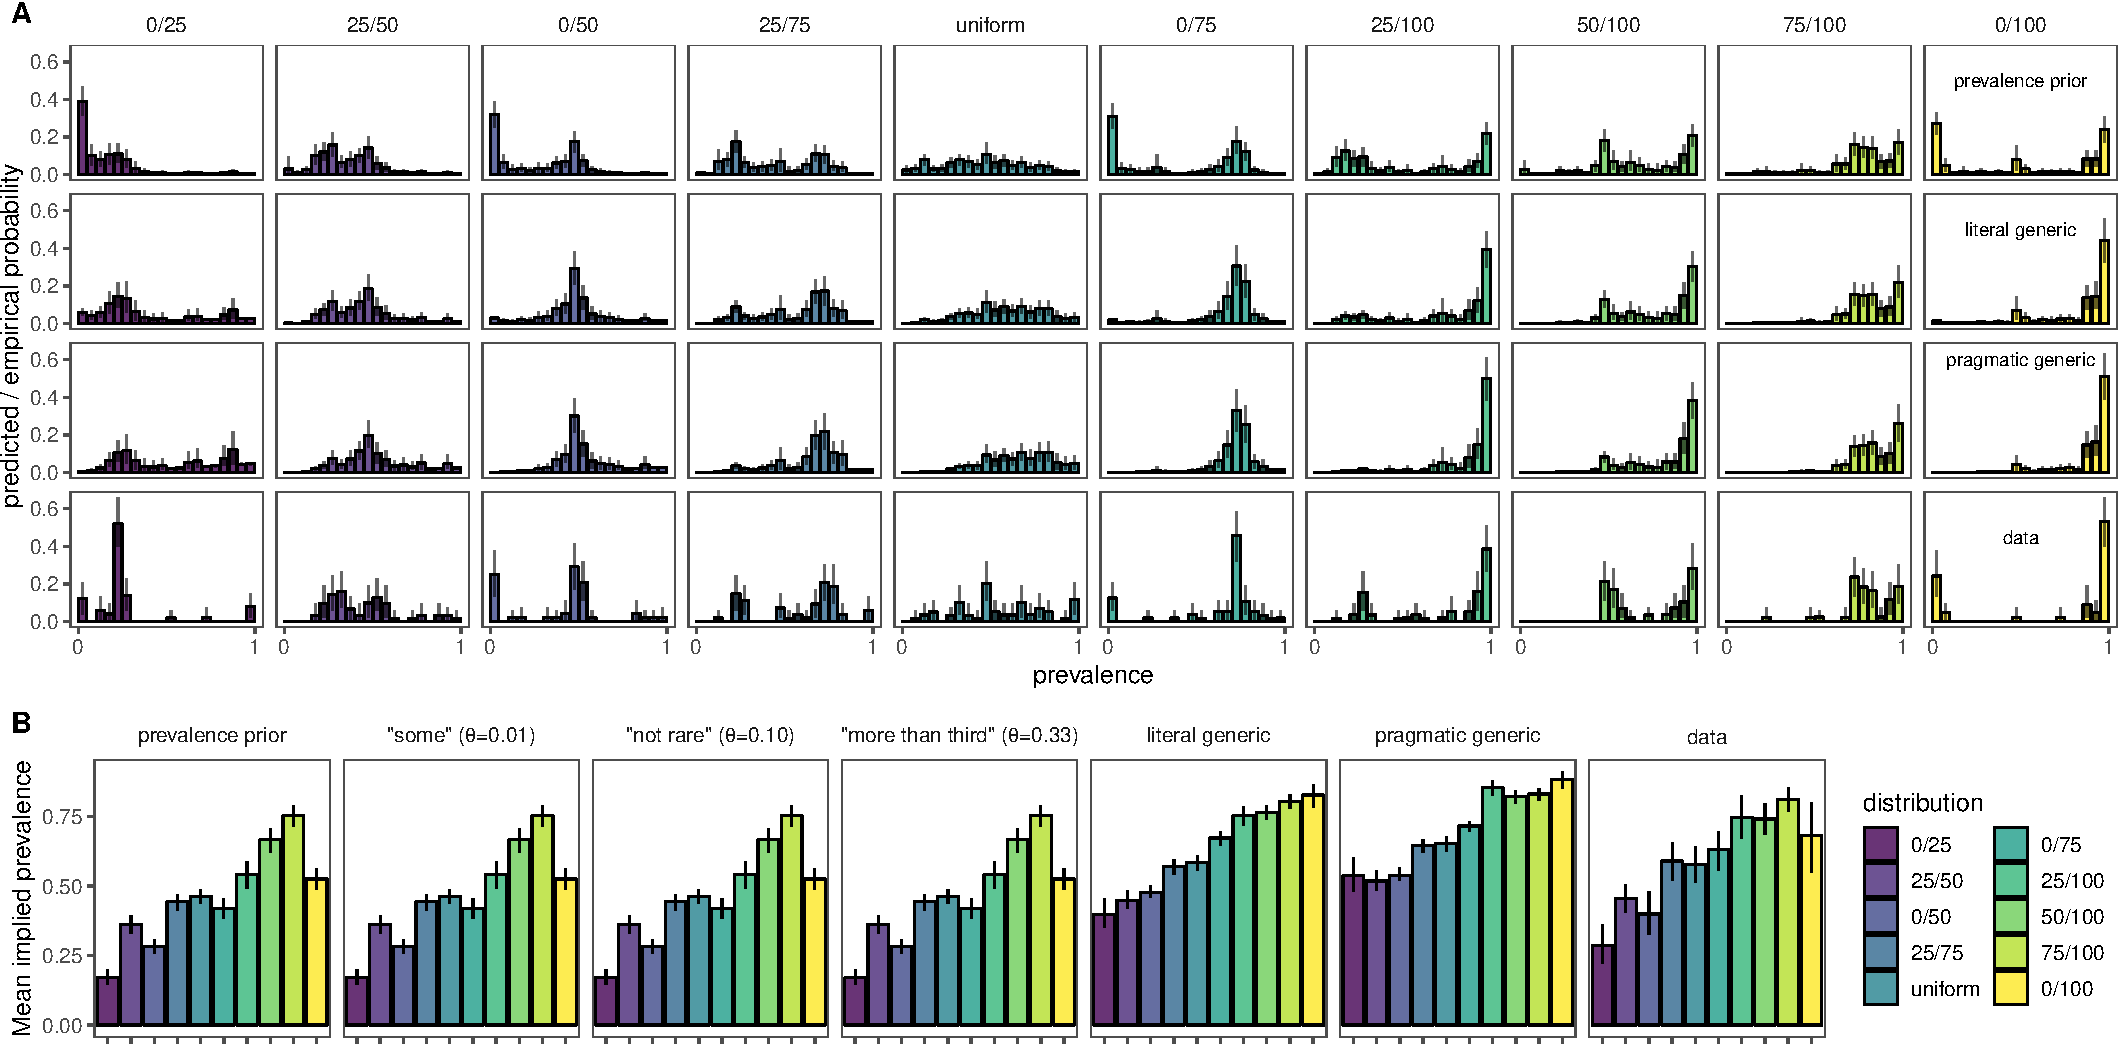
\includegraphics{genint_files/figure-latex/priorManipulationResults-1.pdf}
%\caption{\label{fig:priorManipulationResults}Experiment 2 results. A: Empirical distribution of responses for the prior elicitation task (Expt. 2a; top row), literal and pragmatic generics model predictions based on those empirical distributions (middle two rows), and empirical distributions of responses for the generic interpretation task (Expt. 2b; bottom row). Data and model predictions are shown for ten different prior distribution conditions (horizontal facets). B: Model predicted means for alternative models and empirical means.}
%\end{figure}



\begin{figure}
\centering
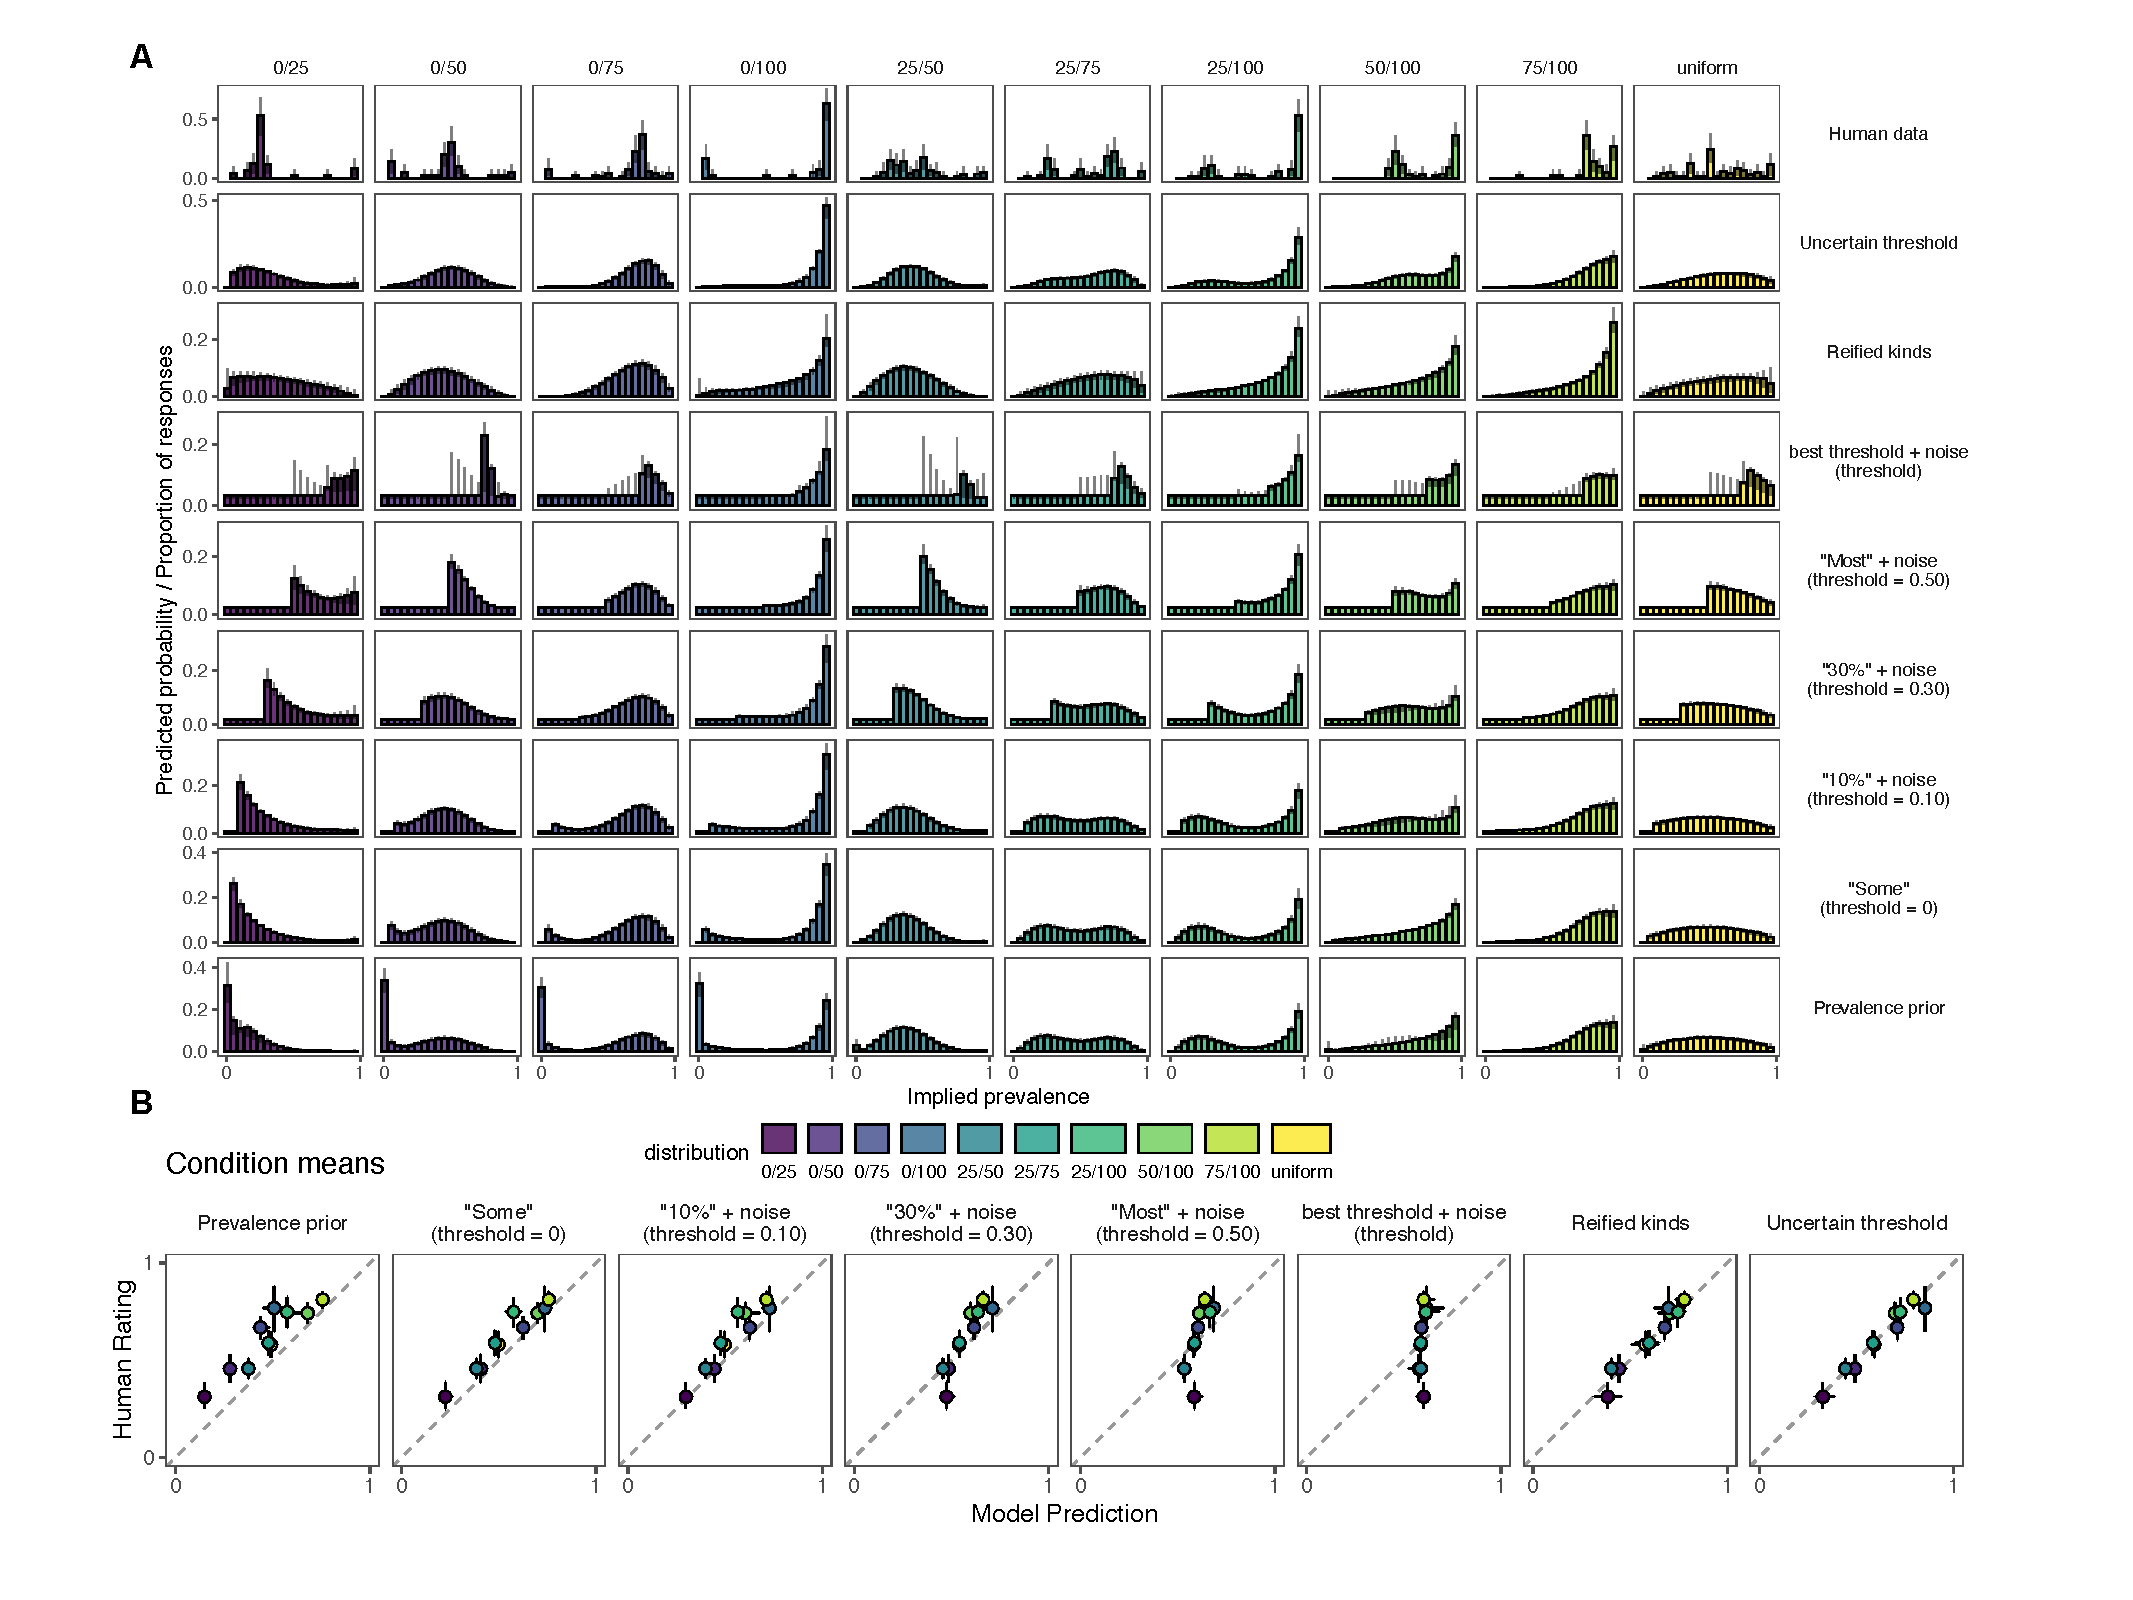
\includegraphics{figs/expt2_model-results_nozero2.pdf}
\caption{\label{fig:genint-modelingResults2}Experiment 3 results. A: Empirical distribution of responses for the generic interpretation task (Expt. 3b; top row), uncertain threshold model predictions, and alternative model predictions. Data and model predictions are shown for ten different prior distribution conditions (horizontal facets). B: Posterior predictive expected values quantitative models in comparison to the human empirical means. Error bars denote bootstrapped 95\% confidence intervals for the behavioral data and 95\% highest posterior density intervals for the model predictions.}
\end{figure}



\hypertarget{results-2}{%
\subsubsection{Results}\label{results-2}}

We used preregistered exclusion criteria, which were also used for Expt. 2a.
Participants who failed to either select the correct property or list a correct number from the familiarization period were excluded (\(n = 39\)).
In addition, we excluded participants who self-reported a native language other than English (\(n = 33\)).
Finally, we employed one exclusion criterion which was not pre-registered: Participants who responded 0\% to the generic interpretation task ($n$ = 18; 3\% of participants); this response is literally impossible under all models of generic interpretation and indicates a misunderstanding of the task. 
A post-hoc analysis of these participants' free-form explanations revealed that the majority of these respondents believed they were responding to a prior elicitation question (predict the next animal); it is likely that these participants were not attending to the generic statement when it was on the screen.
These exclusions left a total of \(n = 514\) participants, with items receiving on average 51 responses (range = {[}40, 62{]}).

Our main qualitative hypothesis is that the same generic sentence (\emph{Ks know when earthquakes are about to happen.}) would be interpreted differently across conditions.
The differences in interpretations are visually evident in the empirical distributions of responses (Figure \ref{fig:genint-modelingResults2}A, top row).
More specifically, we predict that the prevalence implied by the generic sentence will, to a first approximation, track the mean of the prevalence prior distribution.
To test this, we ran a linear model predicting responses with a fixed effect of the prior mean (as estimated by the data from Expt. 2a).
There was a significant main effect of prior mean, with a coefficient close to 1 (\(\beta_1 = 0.94\), \(SE=0.07\), \(t = 12.76\)), indicating a strong linear relationship between the mean of the learned prevalence prior and the resulting interpretations (Figure \ref{fig:genint-modelingResults2}B, left-most facet).
Furthermore, there was a significant main effect of intercept, indicating that participants' responses were significantly greater than the mean of the corresponding prevalence priors (\(\beta_0 = 0.16\), \(SE=0.04\), \(t = 4.44\)).
To more directly test that the distributions of responses in this generic interpretation task (Expt.~2b) were indeed different from the distributions elicited in the prior task (Expt.~1a), we ran exploratory non-parametric Kolmogorov-Smirnoff tests to test for the dissimilarity of the prior and interpretation distributions.  
We found that eight of ten generic interpretation distributions were significantly different than the prior distributions (Table \ref{tab:ks}).
The two which were not significantly different between prior and generic interpretation were the 50/100 and 75/100 distributions. These distributions are also predicted by the uncertain threshold model to be most similar between prior and posterior; since the prior beliefs about prevalence are so strongly skewed towards high prevalence values, the updating power of a generic is more limited.
In summary, these results demonstrate that participants interpret the novel generic sentence in a manner sensitive to the background distribution and that the generic utterance updates participants' beliefs to indicate a prevalence significantly higher than the prior.



\begin{center}
  \begin{table}[h]
    \centering
    \pgfplotstabletypeset[fixed zerofill, precision = 2,
    col sep = comma,
    every head row/.style={before row = \toprule, after row = \midrule},
    every last row/.style={after row = \bottomrule},
    columns/distribution/.style={string type, column name={Distribution Condition}, column type = l},
    columns/D/.style={column name={D}, fixed relative, dec sep, precision = 2},
    columns/pval/.style={column name={$p$-value}, dec sep, precision = 2},
    ]
    {csv_to_tex/expt2_ks_stats.csv}

    \caption{Kolmogorov-Smirnoff test results testing for the dissimilarity between the priors (Expt.~3a) and the generic interpretation (posterior) response distributions (Expt.~3b). The only distributions to be not significantly different between the prior and posterior were the 50/100 and 75/100 distributions; the uncertain threshold model predicts only subtle shifts for these distributions.}
    \label{tab:ks}
  \end{table}
\end{center}


We now rigorously test the uncertain threshold model as a theory of belief updating from generics by asking how it serves the two purposes of a psychological theory: prediction and explanation \cite{shmueli2010explain, yarkoni2017choosing}. 
To test the predictive power of the uncertain threshold model, we can use it and the prior elicitation data (Expt.~2a) to make a number of parameter-free, \emph{a priori} predictions about quantitative differences in mean implied prevalence ratings across the ten distribution conditions.
These predictions were derived by bootstrapping the prevalence prior data to construct bootstrapped 95\% confidence intervals for the uncertain threshold model prediction; from this procedure, we predicted that two conditions should have different mean prevalence ratings if the bootstrapped 95\% confidence interval of the model's predictions did not overlap one another.
With those decision rule in mind, we preregistered the following contrast predictions among mean implied prevalences (conditions within \{\}s indicate a prediction of no difference): 0/25 \(<\) \{25/50, 0/50\} \(<\) \{25/75, \emph{uniform}\} \(<\) 25/75 \(<\) \{25/100, 50/100\} \(<\) \{75/100, 0/100\} (predictions also shown in Table \ref{tab:regResults}).
To evaluate these predictions, we built a Bayesian regression model with the relevant contrasts using a zero- and one-inflated Beta linking function.
The maximum A-Posteriori estimates and 95\% credible intervals of the coefficients of the regression model, as well as the model predicted qualitative differences, are shown in Table \ref{tab:regResults}.
Each of the five predicted positive differences were estimated to be greater than zero, and each of the four predicted null differences were not credibly different from zero.

\begin{table}[h]
\centering
\begingroup\fontsize{10pt}{11pt}\selectfont
\begin{tabular}{llrl}
  \hline
Coefficient & Prediction & Estimate & Credible Interval \\ 
  \hline
Intercept &  & 0.32 & [ 0.221, 0.418] \\ 
  0/25 vs. \{25/50, 0/50\} & $>$ & 0.15 & [ 0.036, 0.278] \\ 
  25/50 vs. 0/50 & = & -0.07 & [-0.270, 0.134] \\ 
  \{0/25, 25/50, 0/50\} vs. \{25/75, uniform\} & $>$ & 0.34 & [ 0.265, 0.409] \\ 
  25/75 vs. uniform & = & 0 & [-0.204, 0.189] \\ 
  \{25/75, uniform\} vs. 0/75 & $>$ & 1.14 & [ 0.903, 1.375] \\ 
  0/75 vs. \{25/100, 50/100\} & $>$ & 1.11 & [ 0.866, 1.352] \\ 
  25/50 vs. 50/100 & = & -0.09 & [-0.297, 0.127] \\ 
  \{25/100, 50/100\} vs. \{75/100, 0/100\} & $>$ & 0.52 & [ 0.307, 0.743] \\ 
  75/100 vs. 0/100 & = & -0.21 & [-0.458, 0.035] \\ 
   \hline
\end{tabular}
\endgroup
\caption{Regression model fits for planned comparisons. Predictions are based on whether the 95\% bootstrapped confidence intervals for the uncertain threshold model prediction overlap.} 
\label{tab:regResults}
\end{table}

To evaluate the uncertain threshold model as an explanation of the data (and in comparison to its its alternatives), we constructed a Bayesian data analysis model to jointly predict the prevalence prior data (Expt.~2a) and the generic interpretation data (Expt.~2b).
As we did for Experiment 1, we model the prevalence prior data for each distribution condition as a mixture of two Beta distributions (with unknown means, variance, and mixture parameters) and we model the generic interpretation via the uncertain threshold model (or an alternative model) that assumes the prevalence prior inferred from the Expt.~2a data (Figure \ref{fig:bayesnet}).
As before, fixed-threshold alternative models make an additional use of a noise parameter to accommodate data points that are literally incompatible with the model. 
To compute the posterior distribution over parameters and generate posterior predictive distributions, we ran for each model 4 MCMC chains consisting of $10^6$ iterations discarding the first $5 \times 10^5$ for burn-in, and checked convergence qualitatively by visual inspection of the parameters and predictions of each chain. 
We additionally performed a formal Bayesian model comparison by computing the marginal likelihood of the data under each model (in order to compute Bayes Factors); to do this, for each model, we collected 1,000 samples from an Annealed Importance Sampling algorithm with an annealing schedule consisting of 50,000 uniformly spaced increments. 

Overall, the uncertain threshold model is the best explanation of the distribution of responses observed in the ten experimental conditions (Table \ref{tab:summary2}). 
For example, in the \emph{0/25} distribution, both the model and participants tend to draw very weak interpretations \emph{a la} the \emph{Some} model, whereas in the \emph{25/100} distribution, the most dominant interpretation is more like \emph{All} (Figure \ref{fig:genint-modelingResults2}).
The model is even able to accommodate subtle shifts in interpretation.
For example, in the \emph{25/75} distribution, most participants interpret the generic as implying roughly 75\% of the category have the property, yet others (a minority) interpret the generic as implying only 25\% have the property. 
This prediction is made by the uncertain threshold model: Higher prevalence levels are more likely under this model, but they are not the only interpretation of the generic; it is plausible that someone could utter this sentence with only in mind that a minority of the category have the property. 
The quantitative details of this kind of weak or inferior inference can also be observed by comparing the 25/100, 50/100, and 75/100 distributions, where there are two kinds of animals, those that always have the property and those that sometimes have the property (where what counts as ``sometimes'' varies between 25, 50, and 75\%). 
Here, the Uncertain threshold model predicts some subset of responses will be at the inferior mode (25/50/75\%) and that the proportion of responses at that inferior mode should increase as the mean of that mode increases (25 $<$ 50 $<$ 75\%), which is also observed in the empirical data. 
This uncertainty in the interpretation data is additionally a reason why the \emph{Reified kinds} model falls short; this model always selects the component of the prior distribution with higher prevalence. 

%We conclude that the prevalence prior is causally related to interpretations of novel generics in the way predicted by the generics models.


%We observe that a number of participants report 0\% of Ks knew when earthquakes were about to happen when they read \enquote{Ks know when earthquakes are about to happen} (Figure~\ref{fig:priorManipulationResults}A, bottom row, \enquote{data}).
%Examining these participants' explanations revealed that the majority of these respondents believed they were answering a slightly different question than the one being asked; they believed they were responding to a question similar to the prior elicitation task: Predict the next animal.
%These \enquote{prior-type} responses are a source of noise in the data that affects all models (except the prior only model) to an equal degree: the models have no way to account for 0\% responses, which are literally impossible given the utterance of the form \enquote{Ks F}.
%%To compute the likelihood of the complete data set under these models, 
%We thus make the further data analysis assumption that the true generative process of the data is a mixture of responding according to one of the generic interpretation models and responding according to the prior.
%In computing marginal likelihood of the data we sum over this mixture parameter in the range of 0-20\% prior-type responses (approximated using the following discretization \(= \{0.001, 0.01, 0.05, 0.1, 0.15, 0.20\}\)).
%%We calculate Bayes Factors assuming a uniform distribution of noise between 0-20\% (approximated using the following discretization \(= \{0.001, 0.01, 0.05, 0.1, 0.15, 0.20\}\)).
%%\ndg{should report posterior CI for this param -- what portion of responses are taken to be prior-type?}
%%\mht{we didn't do a full bayesian analysis of these data; rather the predictions are either 0-parameter predictions based on the empirical priors; the pragmatic predictions are based on a fixed speaker optimality}
%We use this to compute Bayes factors (i.e.~ratio of marginal likelihoods under competing models, discretizing the empirical distributions and model predictions into ten equally spaced bins).
%To account for uncertainty in the measurement of the prior, we again bootstrap the model predictions by resampling the prior.
%As is shown in Table 3, the literal and pragmatic generic interpretation models are best at predicting these data.\footnote{These data do not definitively distinguish the literal and pragmatic models from each other. This is not unexpected, since this experiment was designed to test the causal influence of the prevalence priors and not to distinguish models, which was the goal of the previous experiment.}




%The computational models we have articulated  predict the full distribution of responses, not only the \emph{mean} implied prevalence.
%The model performance in terms of variance-explained and mean squared errors for the full distribution of responses are shown in Table 3.
%(Recall that there are no free parameters fit for this analysis, in any of the models, since we use the best values from the analysis of the previous experiment.)
%
%We next aim to computed the likelihood of the data under each model, to enable model comparison.
%
%While the overall agreement between data and generics models is good, a number of participants 


\begin{center}
  \begin{table}[h]
    \centering
    \pgfplotstabletypeset[fixed zerofill, precision = 2,
    col sep = comma,
    every head row/.style={before row = \toprule, after row = \midrule},
    every last row/.style={after row = \bottomrule},
    columns/model/.style={string type, column name={Model}, column type = l},
         columns/threshold/.style={string type, column name={Threshold}, column type = l},
                   columns/noise/.style={string type, column name={Noise}, column type = l},
    columns/mse/.style={column name={MSE}, fixed relative, dec sep, precision = 2},
    columns/r2/.style={column name={$r^2$}, dec sep, precision = 3},
    columns/log_bf/.style={column name={(log) Bayes Factor}, dec sep, fixed, precision=0}%,
    ]
    {csv_to_tex/expt2_model_summary_stats2.csv}

    \caption{Summary statistics for models of Experiment 2. Mean Squared Errors and variance explained are calculated at the level of the distribution condition means. Bayes Factors quantify evidence in support of each model relative to the Uncertain threshold model and are computed over the full distribution of responses for Expt.~2a \& Expt.~2b. Numbers below 0 indicate evidence in support of the Uncertain threshold model.}
    \label{tab:summary2}
  \end{table}
\end{center}




%\begin{table}[h]
%\centering
%\begingroup\fontsize{9pt}{10pt}\selectfont
%\begin{tabular}{llll}
%  \hline
%Model & log Bayes Factor & expected value statistics & full distribution statistics \\ 
%  \hline
%Prior & -53.9 (-44, -63.6) & r\textsuperscript{2}(10) = 0.91; MSE = 0.0192 & r\textsuperscript{2}(200) = 0.49; MSE = 0.00381 \\ 
%  Threshold = 0.01 & -48.6 (-39, -58.4) & r\textsuperscript{2}(10) = 0.83; MSE = 0.00887 & r\textsuperscript{2}(200) = 0.53; MSE = 0.00358 \\ 
%  Threshold = 0.1 & -26.4 (-17.9, -35.4) & r\textsuperscript{2}(10) = 0.76; MSE = 0.00865 & r\textsuperscript{2}(200) = 0.56; MSE = 0.00334 \\ 
%  Threshold = 0.35 & -48.6 (-39.3, -57.9) & r\textsuperscript{2}(10) = 0.7; MSE = 0.0114 & r\textsuperscript{2}(200) = 0.39; MSE = 0.00485 \\ 
%  Literal Generic & 0 & r\textsuperscript{2}(10) = 0.89; MSE = 0.00429 & r\textsuperscript{2}(200) = 0.64; MSE = 0.00275 \\ 
%  Pragmatic Generic & -2.1 (1.5, -5.6) & r\textsuperscript{2}(10) = 0.82; MSE = 0.0162 & r\textsuperscript{2}(200) = 0.55; MSE = 0.00352 \\ 
%   \hline
%\end{tabular}
%\endgroup
%\caption{Summary statistics for alternative generic interpretations. (Log) Bayes Factors quantify evidence in favor of each model in comparison to the literal generics model. Numbers less than 0 indicate evidence in favor of the literal model. Summary statistics displayed for the model fits for the expected values (means) of the distributions and the full (discretized) distributions. 
%%\ndg{use LL instead of BF here as for previous expt?} \mht{actually LL is misleading here because we are bootstrapping the priors... the range of LLs is large for any given model, but the range of ratios of LL (BFs) is much smaller, because when one model does worse due to a resampled prior, they all tend to do worse}
%} 
%\end{table}


%\begin{table}[h]
%\centering
%\begingroup\fontsize{9pt}{10pt}\selectfont
%\begin{tabular}{llll}
%  \hline
%Model & Log marginal likelihood & Expected value statistics & Full distribution statistics \\ 
%  \hline
%Prior & -403 (-429, -378) & r\textsuperscript{2}(10) = 0.91; MSE = 0.0192 & r\textsuperscript{2}(200) = 0.49; MSE = 0.00381 \\ 
%  Threshold = 0.01 & -397 (-425, -372) & r\textsuperscript{2}(10) = 0.83; MSE = 0.00887 & r\textsuperscript{2}(200) = 0.53; MSE = 0.00358 \\ 
%  Threshold = 0.1 & -375 (-400, -352) & r\textsuperscript{2}(10) = 0.76; MSE = 0.00865 & r\textsuperscript{2}(200) = 0.56; MSE = 0.00334 \\ 
%  Threshold = 0.35 & -397 (-435, -372) & r\textsuperscript{2}(10) = 0.7; MSE = 0.0114 & r\textsuperscript{2}(200) = 0.39; MSE = 0.00485 \\ 
%  Literal Generic & -349 (-372, -326) & r\textsuperscript{2}(10) = 0.89; MSE = 0.00429 & r\textsuperscript{2}(200) = 0.64; MSE = 0.00275 \\ 
%  Pragmatic Generic & -351 (-375, -328) & r\textsuperscript{2}(10) = 0.82; MSE = 0.0162 & r\textsuperscript{2}(200) = 0.55; MSE = 0.00352 \\ 
%   \hline
%\end{tabular}
%\endgroup
%\caption{Summary statistics for alternative generic interpretations. (Log) Bayes Factors quantify evidence in favor of each model in comparison to the literal generics model. Numbers less than 0 indicate evidence in favor of the literal model. Summary statistics displayed for the model fits for the expected values (means) of the distributions and the full (discretized) distributions. \ndg{use LL instead of BF here as for previous expt?}} 
%\end{table}

\hypertarget{general-discussion}{%
\section{General Discussion}\label{general-discussion}}


%\red{SOcial import, minimal example (property)
%L0: predicate observed, all other features missing
%language is hard for actually describing specifics
%think about hte law
%good for minimal examples
%}

Generic language is the foremost case study of how abstract, generalizable knowledge is transmitted through language.
%, and it is commonly believed that generics carry strong interpretations (analogous to the quantifier \enquote{most} or \enquote{all}).
Despite their ubiquity and relative morphosyntactic simplicity, generics have been examined by few quantitative studies and no quantitative models that make predictions about how generic language updates beliefs.
Here, we explored the hypothesis proposed by \citeA{Tessler2019psychrev} that generics update beliefs according to an uncertain threshold semantics. 
We tested these models using a diverse set of stimuli and showed that the generic interpretations can be predicted with high-quantitative accuracy as a function of background knowledge about the property updated by an uncertain threshold rule (Experiment 1).
In Experiment 2, we showed how model also explains extant differences observed from the previously published work of Cimpian et al. (2010).
Furthermore, we found that the background knowledge about the expected prevalence of the feature was causally responsible for how novel generic statements get interpreted (Experiment 3).
%Our data strongly support the conclusion that generics can be thought of as conveying quantitative information about the prevalence of the property in the category. 
% The information content, however, is not derivable outside of context; the meaning of generic statement manifests via reasoning about what threshold would be likely to be true given background knowledge about the property.
% interprets generics pragmatically provides a better explanation of the observed data than a literal interpretation model.
This work validates a computational formalism to articulate how beliefs are updated from generic language, which appears to be adequate within the domains considered; it represents a first step in understanding how generics serve to convey knowledge between people and generations.


%
The experimental data we present shows that generics can receive a systematic spectrum of prevalence-based interpretations, including being interpreted as only applying to a minority of the category (what we might call \emph{weak generics}). 
Statements like \emph{Lorches live in zoos}, \emph{Feps perform in the circus}, and \emph{Wugs have seizures} all received average implied prevalence ratings below 50\%, with many individual participants providing ratings of 10\% or less (Expt. 1b).
When manipulating the prevalence prior distributions to suggest only prevalence levels of around 0\% or around 25\%, participants readily interpret the statement \emph{Ks know when earthquakes are about to happen} to mean about a quarter of them do (Expt. 3b).
%These nuanced interpretations are an aspect of generic language understanding often swept under the rug: Generics are believed (in a generic sense) to carry strong implications.
These results highlight the variety of generic interpretations, which stand in contrast to a common view in the psychological literature on generics that generics (in a generic sense) convey monolithic, strong meanings.
Here, we trace the variability of generic interpretations back to prior beliefs, demonstrating how generics can convey strong implications, weak implications, and all shades in-between.\footnote{
The response measure we use in our paradigm, as in the previous paradigms on generic implications, might encourage gradience even if gradience was limited.
For example, \citeA{armstrong1983some} showed that one can elicit gradience from objectively binary properties (e.g., the ``evenness'' of numbers).
Gradience in property prevalence interpretations (e.g., how many wugs have seizures), which we examine in this paper, is distinct, however, from gradience in property knowledge (e.g., whether or not an individual instance or episode could be a gradient exemplar of a property such as a seizure). Our results cannot speak one as to whether or not property knowledge \emph{per se} is gradient, just that knowledge of prevalence is gradient. Prevalence knowledge being gradient is not particularly surprising given that the underlying construct is itself gradient (i.e., prevalence is a probability or frequency, which is a number between 0 - 1). 
}

\subsection{Generics, statistics, and concepts}


A dominant view in psychology is that the meaning of generic statements cannot be reduced to statistical information about the prevalence of the feature in the category \cite<e.g.,>{Leslie2008, Cimpian2010, Khemlani2012, Prasada2013}. 
This conclusion is often arrived at by only considering fixed-threshold models of a prevalence-based semantics.
Our comparisons to models that assume fixed-thresholds support this narrow conclusion, that a fixed-threshold semantics for generics is difficult to support given the data.
The broader conclusion --- rejecting all possible semantic models based on prevalence --- is not warranted, however (see also \citeNP{kochari2020generics} for a similar argument).
The meanings of many expressions in natural language depend inextricably on context. 
For example, gradable adjectives like \emph{tall} or \emph{expensive} do not convey a single precise quantity of height or price (e.g., an expensive watch is probably a different price than an expensive hamburger), and yet we do not conclude from that the core meaning of \emph{tall} has nothing to do with height or that the meaning of \emph{expensive} is not really about the price of the object.
The meanings of gradable adjectives are often arrived by considering a comparison class of other objects of the same type \cite<e.g., an expensive hamburger is one that has a price that is high relative to other hamburgers;>{Kennedy2007} or which is pragmatically felicitous \cite{Tessler2017}, and the meaning of vague adjectives can be modeled using an uncertain threshold in a way completely analogous to how we have modeled the meaning of generics \cite{Lassiter2015}.
Therefore, we conclude that quantitative, prevalence information can be at the core of generic meaning, but that such a meaning must be vague and context-sensitive (see also \citeNP{Sterken2015, Nickel2016} for related ideas about context-sensitivity of generics, and see \citeNP{vanRooij2020generics} for a mathematically similar account of generics).

At the same time, generics are known to influence conceptual knowledge.
The fact that generics refer to abstractions has pinpointed them as potentially central to the growth of conceptual knowledge \cite{Gelman2003, Gelman2009}, such as intuitive or folk theories of biology or psychology \cite{carey1985conceptual, gopnik1997words}. 
Generics can also encode normative beliefs about objects or people \cite{gockeritz2014young, roberts2017group, orvell2018s}. 
In our model of generics, conceptual changes can occur at a higher level of abstraction above our minimalist, prevalence prior representations of world knowledge (e.g., the prevalence prior may be a lower-level variable in a rich, generative model of kinds and properties \emph{a la} \citeNP{kemp2012integrated}). 
That is, the prevalence prior is an intermediate representation between conceptual knowledge (e.g., which could encode normative beliefs) and truth-functional semantics with a quantifiable, unified metric to evaluate whether a statement is true or false. 
Our model does takes the strong view that the mechanism by which generics influence conceptual beliefs is via beliefs about prevalence or probability. 
This view may turn out to be incorrect (e.g., a notion of value could also be a part of the core meaning of generics, as formalized by \citeNP{vanRooij2020generics}), but in our three heterogenous data sets that we have modeled and presented here, we do not see any gap between the uncertain threshold model predictions and the empirical data, suggesting that prevalence alone in the semantics of generics is sufficient.


\subsection{Generics as a vehicle for cultural transmission}

The model we examined closely in this paper was first proposed as a listener model embedded inside of a pragmatic speaker model designed to predict generic endorsements, or truth judgments \cite{Tessler2019psychrev}.
\citeA{Tessler2019psychrev} showed that the generic endorsement judgments (e.g., do you endorse the statement:  \emph{Mosquitos carry malaria}?) can be predicted this speaker model deciding whether or not to produce the generic to a naive listener, where the naive listener updates its prior beliefs via an uncertain threshold function. 
We show here that the model of the naive listener---the \emph{Uncertain threshold model}---perfectly tracks with the generic interpretation data (Expt.~1b, 2b, 3b), in a manner that closely resembles how the predictions of the  speaker model of \citeA{Tessler2019psychrev} closely tracked with the variability among generic endorsements.
Taken together, this pair of results---the speaker model of \citeA{Tessler2019psychrev} predicts generic endorsements, and the listener model (about which the speaker model reasons) predicts generic interpretations---points to a more general conclusion that our unified, model-based approach warrants: Generic endorsements and interpretations behave as one would expect if speakers and listeners are rational users of language. 
More broadly, speakers and listeners use and interpret generics in a manner indicative of a mechanism for faithful transmission of knowledge \cite{Tomasello1999}. 
That is, at least for our set of stimuli, listeners interpret generics in the ways that speakers intend.
This conclusion supports the role of generic language in the broader toolkit for human cultural transmission \cite<see also>{tomasello2016cultural, gelman2017language}.

%The conclusion that generics are a mechanism for faithful transmission of knowledge

There are some important features of our paradigm that make our experiments a kind of ``best case'' scenario for finding evidence for faithful knowledge transmission and should be taken into account to understand the generalizability of this conclusion. 
Foremost, is that our stimuli are all generics about animals categories and properties, the statistics of which are relatively common knowledge and uncontroversial.
For features that have difficult-to-understand statistical properties \cite<e.g., features of social categories;>{judd1991accuracy}, prior beliefs about the prevalence of features can easily be misaligned between any individual pair of speaker and listener, potentially leading to the propagation of misinformation or stereotypes \cite<see also>{roberts2017group}.
A second crucial feature of our designs that impact the generalizable of this conclusion is that our studies are all done with adults.
The usage of generics as a mechanism of transmitting knowledge to children may also result in unfaithful transmission due to different prior beliefs throughout development \cite<e.g.,>{brandone2017changes}.
Testing the \emph{Uncertain threshold model} (and the speaker model component in \citeNP{Tessler2019psychrev}) with generics about socially sensitive topics and in development are important future directions for this approach.


%This notion of faithful transmission of knowledge stands in opposition to previous reports of an ``asymmetry'' between endorsements and interpretations \cite{Cimpian2010}. This work, however, relied on an intuitive model for how generics 
%Without a precise model for how generics should update beliefs and how generic endorsements are made, 





%Rather than view , we show that generics also carry weak implications and all shades in-between.

%\mht{Describe arguments against fixed-threshold, classical views in psychology}

%\mht{
%\begin{enumerate}
%\item relationship to single observation
%\item conceptual interpretations
%\end{enumerate}}

%The model of the literal content of a generic as conveying a single, positive observation is mathematically equivalent to the interpretation model assumed by Tessler \& Goodman (2019) where the generic acts a vague quantifier (Appendix A). 
%The generics-as-vague-quantifier formulation is similar to a Rational Speech Act model proposed by Lassiter and Goodman (2017) for interpreting context-sensitive, scalar adjectives (e.g., \emph{tall}).
%Lassiter and Goodman (2017) argued that the truth-functional threshold (i.e., the literal point at which something becomes tall) ought to be reasoned about by the pragmatic listener: That is, their model ``lifts'' the threshold variable to the pragmatic listener to allow communicative reasoning to influence the value of the threshold (e.g., the listener reasons about what thresholds would be informative) in a style consistent with other ``lifted variable'' RSA models (see Goodman \& Frank, 2016 for a review). 
%Our pragmatic model of generics does not reason about the threshold; in fact, the generics-as-single-observation version of the model no longer makes reference to a threshold variable. 
%Instead, our model is analogous to a Lassiter \& Goodman (2017) style model where the threshold variable is only present at the level of the literal listener and is integrated out of the model prior to any pragmatic reasoning. 
%That being said, the predictions of these two versions of a pragmatic generics model are only very subtly different from one another, and we omit a detailed comparison of these models for brevity. 

\hypertarget{the-relationship-between-prevalence-priors-and-generic-interpretations}{%
\subsection{The relationship between prevalence priors and generic interpretations}\label{the-relationship-between-prevalence-priors-and-generic-interpretations}}

%{\textcolor{Green}{[ndg: people may worry about circularity of argument, given rich background knowledge elicitation that also uses language (similar to ellen's point). i think we should discuss this directly. relatedly we should discuss the implications of our structured background knowledge (elicitation and results).]}}
%{\textcolor{Blue}{[mht: does this address it?]}}

In our experiments, we predict participants' implied prevalence ratings with our computational model as a function of empirical measurements of participants' background knowledge about properties, specifically background knowledge about the prevalence of properties. 
%The background knowledge elicitation tasks involve reasoning about the properties of alternative categories of animals.
%In order to elicit this knowledge, however, we conveyed instructions and questions using language. 
%Thus, there is the potential for circularity in our argument: We are predicting beliefs updated from language via beliefs elicited from language.
%A close inspection of the prior elicitation questions and our control quantitative models argue against circularity, however. 
%Our argument is not circular, however, because of the nature of the prior elicitation questions and our control quantitative models, which we describe below.
In Expt. 1a, we elicited background knowledge by having participants first generate different animal categories and then later rate prevalence for different properties of those animals.
One might worry that there is a potential for circularity because we are predicting beliefs updated from language (\emph{generic interpretation}; Expt.~1b) via beliefs elicited partly from language (\emph{prevalence prior}; Expt.~1a).
Perhaps participants answer the prevalence prior questions (e.g., \emph{What percentage of dogs develop phobias?}) by first asking themselves internally a generic question (\emph{Do dogs develop phobias?}) and then  if the answer to this question was \emph{yes}, responding with their personal (already generically-interpreted) prevalence (and rating 0\% prevalence if the answer to the generic question was \emph{no}).
This procedure would be consistent with a view of generics as representationally primary (as posited by \citeNP{Prasada2000} in the form of \enquote{generic beliefs}) and in which prevalence estimates are derived by these \enquote{generic beliefs}. 
%Furthermore, under this view, the generic interpretation task (Expt.~1b) reduces to simply reporting back the part of the prior distribution that was generated when participants answered \enquote{yes} to their internally-directed generic question in the prevalence  prior task (\enquote{Do dogs develop phobias?}).
Under this view, the two experiments would be measuring essentially the same construct, with the latter experiment (\emph{generic interpretation}; Expt.~1b) restricting to  kinds that generically have the property. 

%Several aspects of our data argue against this possibility. 
Our formal model comparisons provide strong evidence against this interpretation.
First, the \emph{Some} model---which updates the prior by ruling out the 0\% prevalence part of the distribution---is a simple control model that captures the reasoning articulated above: If there is an inherently binary kind of reasoning occurring (``kinds either do not do not [generically] have the property''), we would expect updating the prior by removing the 0\% prevalence part of the distribution to return whatever it means to ``generically have the property''. 
%Foremost, the prevalence priors do not seem to be a simple mixture of two distributions (e.g., \emph{generically do and do not have the property})---we needed to model each distribution as a mixture of three distributions because they exhibit complex structure. 
%Second, if the above strategy were that employed by participants, the most accurate model for the generic interpretation data should be the existentially-quantified
The \emph{Some} model consistently under-predicts the generic interpretation data, however, and was easily ruled out by model comparison given our data.
An even more sophisticated version of this hypothesis is formalized by the \emph{Reified kinds} model, which explicitly reasons about the prevalence in a kind of binary fashion: It looks at the prior as a mixture of two distributions (intuitively, the ``haves'' vs. the ``have nots'') and selects the distribution with the higher mean prevalence value (the ``haves'').
While the predictions of this model closely track the predictions of the \emph{Uncertain threshold} model for many generics, the \emph{Reified kinds} model over-predicts the prevalence ratings for generics that convey weak interpretations (e.g., \emph{Dorbs live in zoos.}) and is ruled out consistently by the data via formal model comparison. 
In addition, the \emph{Reified kinds} model is unsatisfactory from a theoretical perspective because it ties the meaning of a generic to a particular structural assumption about world knowledge (e.g., the prevalence prior as a mixture distribution). 
These results support the idea that belief-updating from generics is more nuanced that simply fixing the binary value of a \emph{generic belief} node to be true (cf., Prasada, 2000; Csibra and Shamsudheen, 2015).
Instead, it is most parsimonious to conclude that from these experiments that generics update prior beliefs about prevalence in a graded fashion, modeled as an uncertain threshold rule.
%If this were the case, there are only two possibilities for participants' beliefs---the category either does or does not (generically) have the property---and the generic interpretation task 
%
%
%The fact that the \enquote{some} model consistently underpredicts the generic interpretation data argues against the circularity in our measurements of the prevalence prior and generic interpretations.


\subsection{Generics and pragmatics}

The \emph{uncertain threshold} model of generic interpretation that we test and validate this paper is a kind of \emph{Literal Listener} model used in a probabilistic models of pragmatic language use (e.g., the Rational Speech Act theory; \citeNP{Frank2012, Goodman2016, problang}). 
It is noteworthy that we are able to predict the inferences from generics in these experiments without having to articulate a full-blown model of pragmatic reasoning (i.e., a \emph{Pragmatic Listener} model). 
In the course of this project, we formalized and tested two different versions of a pragmatic listener model. \footnote{Specifically, we formalized a model that treated the threshold variable as a ``lifted'' variable subject to recursive pragmatic reasoning (analogous to \citeA{Lassiter2015}'s model gradable adjective interpretation) and another which marginalized out the threshold variable before engaged in recursive reasoning.}
The predictions of these pragmatic listener models were only subtly different than the literal listener model and we found that the models provided comparable fits to the data in comparison to our literal listener model, but where penalized in the model comparison due to their additional flexibility in the kinds of data they could predict (i.e., the pragmatic models were more flexible due to their structure and an additional free parameter governing the rationality of the hypothetical speaker who produced the generic). 

Our observation that the predictions of the pragmatic listener models and the literal listener models were only subtly different suggests that an experiment likely needs to be designed specifically to arbitrate between these hypotheses in order to distinguish them.
Such a paradigm should probably move beyond the artificial, hypothetical situations studied here and in previous work on generic interpretations. 
For example, an interactive paradigm where a listener can understand that a speaker produced a generic as an intentional action may be more well suited to tap into the perceived intents of the interlocutors. 



%The model as we have articulated in this paper derives a problematic interpretation of the generic that A produces.


%Similarly, the patterns of data we observe in our experiments are additionally unlikely to be identical to those obtained using the quantifier \enquote{Some} (i.e., \enquote{Some Ks have F}).
%Though we did not empirically measure judgments given the existentially quantified statements, the alternative model that assumes a fixed-threshold at 0\%-prevalence provides insight into what should be expected for those data.\footnote{Recall the fixed-threshold models are \enquote{literal interpretation} models and do not compute scalar implicatures.}
%In both of our experiments, we found that the \enquote{some} model provided too weak of interpretations, consistent with the intuition that generic statements convey stronger prevalence implications that the existential statement.

%A similar argument can be made for the structured elicitation task in Expt. 1a.
%In Expt. 1, we assumed a particular model of the prevalence prior (i.e., a mixture of Betas) and elicited participants' knowledge about the property using questions that we assumed tapped into this structure.
%One question concerned the probability that a kind would have 0\% prevalence of the feature (or, equivalently, the proportion of categories for whom the property is expected to be present at some non-zero level of prevalence) by asking \enquote{How likely is it that \emph{there is a K with F}?}
%Intuitively, the response to such a question should be that it is very likely for properties that exist in many categories (e.g., \emph{is female}) and very unlikely for properties that only exist in a few categories (e.g., \emph{has purple feathers}).
%The second question concerned the shape of the non-zero conditional distribution of prevalence; this was measured by asking \enquote{\emph{Suppose there is a K with F}, how many Ks do you think have F?}.
%This question measures the projectibility of the property given a single, positive exemplar.
%Thus, the predictions of the alternative, fixed-threshold \enquote{some} model (which rules out 0\% prevalence) for this experiment correspond to the inferences upon learning that \emph{at least one member of the category has the property}.
%In Expt. 1, we again find the generic interpretation data are distinct from those of the conditional, non-zero distribution of prevalence, as evidenced by the \enquote{some} model comparisons.
%The fact that we use this \enquote{single, positive observation} question to elicit prior knowledge may in fact have blurred the distinction between the literal and the pragmatic model, which is why we Expt. 2 was conducted.


%Another interesting question is whether the same pattern of data could arise from a bonafide pedagogically sampled observation (cf., Csibra \& Shamsudheen, 2015).
%Given the success of the pragmatic model, we suspect this is possible, provided the pedagogical example is a minimal example. 
%We also suspect, however, an interaction with the alternative actions available to the speaker or teacher.
%That is, we do not expect bonafide generic interpretations from pedagogical demonstrations when the speaker could have said a generic.
%Finally, it should be noted that many of the properties used in our experimental stimuli are not directly observable either due to the nature of the property (e.g., \enquote{transmit HIV}) or to the habituality of the predicate (e.g., \enquote{fly into building windows}).


%\subsection{Weak generics and the danger of asymmetry}

%The fact that understanding generics relies heavily on background knowledge about properties provides a clear avenue for miscommunication when using and learning from generics.
%Cimpian et al. (2010) provided evidence for an \emph{asymmetry} between the conditions that permit a speaker to assert a generic and the prevalence learned by the listener from that same statement. 
%The situation arises if a speaker endorses a generic when the prevalence is quite low, believing that they and the listener share the background assumptions that the property is a low-prevalence property in general (see Tessler \& Goodman, 2019 for the relevant model of speaker endorsement of generics).
%To the extent that a listener has a different set of assumptions of the distribution of the property, miscommunication will result.
%%For many properties, the difference in implied prevalence may be inconsequential.
%We saw that the biggest differences between the literal interpretation model (which guides the predictions of the generic speaker model used in Tessler \& Goodman, 2019) and the pragmatic generic interpretation model occur when the distribution of the property is most uncertain.







%Adults flexibly use their causal knowledge of the world to restrict the interpretation of a generic statement to a reasonable population, as evidenced by their explanations (e.g., \enquote{I thought that there would be many more Dobles in the wild than in zoos}).
%At the same time, the communicative force of a generic encodes a pressure for higher prevalence interpretations (e.g., without strong prior knowledge, generics imply high prevalence).
%Thus, listeners who do not have the substantial prior knowledge to restrict an interpretation of generics to a weak interpretation (e.g., young children) might derive a high-prevalence interpretation and furthermore posit abstract relations that would make a high-prevalence interpretation more likely.
%For example, upon learning \enquote{Dobles live in zoos}, a naive learner might infer that there is something about Dobles that causes them to live in zoos (cf., Prasada, Khemlani, Leslie, \& Glucksberg, 2013).
%This is potentially problematic for language about social categories (e.g., \enquote{Tall people are good at basketball}) for which an adult speaker might wish to convey a relatively low prevalence interpretation (e.g., \emph{some tall people\ldots{}} because most people are not good at basketball) but which a naive listener might derive a higher prevalence interpretation.
%This points to an aspect of generic meaning that might differ between adults and children: Whether or not children understand weak generics.



%The fact that an underspecified quantifier semantics proposed by Tessler and Goodman (2019) is equivalent to an observation model provides a route to learning the truth-functional meanings of natural language expressions through analogy to a more general learning mechanism. 
%That is, an uncertain quantifier updates beliefs in exactly the same way as a single positive observation. 


%\mht{What is Leslie's ``default generalization'', then? A single pedagogical observation}

%\mht{what do the words in the generic do? they point to the features that are relevant in the observation, kind of analogous to a demonstrator exaggerating their actions when producing a demonstration. they also point to the category to generalize (though, the actual category to generalize may be a restricted class (e.g., ``cabs are yellow'' [NYC cabs])}

%\mht{generics come in diverse syntax (within and across languages). ``A dog barks'' literally means one dog barked. ``You see a dog, it barks'' has the same semantics as both a particular and a generic?}


%\mht{another model: $x^n$ semantics... probably computationally indistinguishable as well}

%\mht{why is a single positive observation model different than the ``some'' model? ``some'' just tells you that both sides of the coin are not tails. gen tells you that you flipped it and it came up heads...}




%In what follows, we elaborate the assumptions in our modeling framework, describe how conceptual knowledge can guide prevalence-based interpretations, discuss how our answer to the problem of generic interpretation can inform an answer to the parallel problem of \emph{generic identification}, and speculate about the implications for communicating weak generics.
%

%{\textcolor{Green}{[ndg: i'm not so sure about including these following discussion sections. they seem like interesting but only thematically related, as apposed to being crucial to our story or responses to probably objections. i didn't comment / edit them yet -- let's first decide if they stay.]}}
%
%
%\hypertarget{conceptual-generic-interpretations}{%
%\subsection{Conceptual generic interpretations}\label{conceptual-generic-interpretations}}
%
%In this paper, we tested a particular model of generic interpretation that uses a prior distribution over the prevalence of a feature across relevant categories and assumes the truth-functional meaning of the generic is an uncertain threshold on the prevalence.
%The prevalence prior distributions, which we elicit from participants, are likely influenced by the conceptual knowledge of our participants.
%For example, the prevalence priors over properties that have to do with reproduction (e.g., \emph{have menstrual cycles}, \emph{get erections}) are multi-modal with one mode around 50\%, clearly reflecting participants' biological knowledge that these properties are specific to one sex of the animal.
%We thus predict that 4-year-olds, who lack significant biological knowledge (Carey, 1985), would derive different interpretations than adults from generics about these properties.
%
%Consistent with the intuition that conceptual knowledge underlies prevalence judgments, participants appeal to domain knowledge in their explanations for low-prevalence ratings, revealing aspects of their intuitive theories which guide their judgments.
%One participant wrote: \enquote{About half are females and females have menstrual cycles.}
%Another: \enquote{I assumed that only a percentage of Moxes were female and young enough to have a menstrual cycle.}
%A typical explanation of a participant's response to \emph{Dobles live in zoos} was \enquote{I thought that there would be many more Dobles in the wild than in zoos. This is true of most animals in zoos today}.
%Here, it is clear that the participant is using their knowledge of the property, derived from other animals, to learn about the category.
%Participants often wrote about the lack of an enabling causal situation when describing their weak interpretations: \enquote{Most frams don't have access to nicotine.}
%Explicitly modeling the intuitive theories that give rise to the intuitions about prevalence is an obvious future direction of this work.
%
%Other semantic theories of generics make use of a mechanism by which the domain over which the prevalence of the feature in the category is calculated is contextually restricted (e.g., Cohen, 1999; Declerck, 1991).
%In such a theory, the statement \enquote{Morseths have a menstrual cycle} gets evaluated as \enquote{Female morseths have a menstrual cycle}; under such an account, the implied prevalence of the feature would be 100\% (or near 100\%) because 100\% of the \emph{relevant lorches} (i.e., the females) have a menstrual cycle.\footnote{The scientifically correct term for a \enquote{menstrual cycle} is actually an \enquote{estrous cycle}. We are grateful to one of our MTurk participants for pointing this out to us. }
%Interestingly, domain restricted interpretations are present in the empirical data.
%Several properties about the reproductive behavior of animals (Expt. 1b) have interpretation distributions that are bimodal.
%For example, \enquote{Morseths have a menstrual cycle} is interpreted primarily as applying to 50\% of morseths (38 out of 64 give a response between 45\% and 55\%); however, some participants (10 of 64) rate this as applying to 100\% of morseths.
%This behavior could result from a participant interpreting the question as pragmatically restricting the domain to only the members of that category that \emph{could} have the property (e.g., 100\% of female morseths have a menstrual cycle).
%The domain restricted interpretation is not limited to the generic interpretation data, however.
%The bimodality is present in our prevalence elicitation task (Expt. 1a) as well: The distribution over several of the reproductive properties is tri-modal, with peaks at 0\% (the animals that don't have a menstrual cycle), 50\% (\enquote{only females}) and 100\% (perhaps, \enquote{all females}).
%The fact that this multi-modality appears in the prior elicitation task means that the generic interpretation model predicts bi-modal interpretation distributions for the implied prevalence data, which is what we observe.
%Still, the question remains why some participants interpret the noun phrase in generic statements as restricted to a salient subset of the category.
%
%


%\hypertarget{generic-identification}{%
%\subsection{Generic identification}\label{generic-identification}}
%
%{\textcolor{Blue}{[mht: i think this should be cut... unless you think there is something here?]}}
%
%Though often interpreted as generics, bare plural sentences (e.g., \enquote{Dogs bark}) can also manifest as \emph{non-generics} (e.g., \enquote{Dogs are on my front lawn}).
%Figuring out when a sentence expresses a generic meaning vs.~a non-generic meaning is called the problem of generic identification and is a parallel challenge to the problem of generic meaning (Carlson \& Pelletier, 1995).
%Our answer to the question \enquote{what do generics mean?} involves vagueness concerning the prevalence, which recruits beliefs about the property in question.
%The properties themselves may involve vagueness in terms of genericity, or its event counterpart \emph{habituality}, such as \emph{barks}: How often does an individual dog need to bark in order to qualify as a thing that barks?
%Tessler and Goodman (2019) showed that the same uncertain threshold mechanism explains graded endorsements of habitual statements like \enquote{John's dog barks}.
%
%The habituality of the predicate may actually be the source of the perceived generic/non-generic distinction.
%For instance, \enquote{Dogs are on my front lawn} exhibits only a single generalization (e.g., over \emph{dogs}); it is not a habitual predicate like \emph{barks}.
%The habituality of the predicate may influence the expected prevalence in the head noun category: A more vague, habitual predicate may be applied by human observers to more instances of the category because it is harder to verify than static properties.
%For non-habitual predicates, the expected prevalence would be substantially more restricted.
%Thus, we may find continuity in interpretations of underspecified noun phrases, including so-called \enquote{non-generics}: \enquote{Tigers have stripes} has higher implied prevalence than \enquote{Tigers are in the savanna} which is higher than \enquote{Tigers are in zoos}, \enquote{Tigers are in my local zoo}, and \enquote{Tigers are on my front lawn}.
%An uncertain threshold mechanism of the kind we have posited here may be such a way as to pragmatically infer a continuum of interpretations, from generics that are interpreted as universals (\enquote{Tigers are mammals}) to those that are interpreted existentially but habitually (\enquote{Tigers are in zoos}) to those that are interpreted existentially and non-habitually (\enquote{Tigers are on my front lawn}).
%Deriving such a prediction would necessarily involve a model of compositional generic interpretation, in which a habitual predicate meaning can be resolved jointly with a generic subject.


\hypertarget{conclusion}{%
\subsection{Conclusion}\label{conclusion}}

An easy way to acquire abstract knowledge is to understand a generic statement produced by a helpful interlocutor. 
A computational model that understands generics as operating as a vague quantifier is able to predict the large variability in generic interpretations.
This work provides further support for a computational approach to generic language, opening the door to understanding more precisely how abstract knowledge is learned from language and conveyed through generations.

\newpage

%\hypertarget{references}{%
%\section{References}\label{references}}
\bibliographystyle{apacite}

%\setlength{\bibleftmargin}{.125in}
%\setlength{\bibindent}{-\bibleftmargin}

\bibliography{generics}
%\hypertarget{refs}{}
%\leavevmode\hypertarget{ref-Abelson1966}{}%
%Abelson, R. P., \& Kanouse, D. E. (1966). Subjective acceptance of verbal generalizations. In S. Feldman (Ed.), \emph{Cognitive consistency: Motivational antecedents and behavioral consequents} (pp. 171--197). Academic Press.
%
%\leavevmode\hypertarget{ref-Baker2009}{}%
%Baker, C. L., Saxe, R., \& Tenenbaum, J. B. (2009). Action understanding as inverse planning. \emph{Cognition}, \emph{113}, 329--349. doi:\href{https://doi.org/10.1016/j.cognition.2009.07.005}{10.1016/j.cognition.2009.07.005}
%
%\leavevmode\hypertarget{ref-carey1985conceptual}{}%
%Carey, S. (1985). \emph{Conceptual change in childhood.} Cambridge, Massachusetts: MIT Press.
%
%\leavevmode\hypertarget{ref-Carlson1977}{}%
%Carlson, G. N. (1977). \emph{Reference to kinds in english} (PhD thesis). University of Massachusetts, Amherst.
%
%\leavevmode\hypertarget{ref-Carlson1995}{}%
%Carlson, G. N., \& Pelletier, F. J. (1995). \emph{The generic book.} Chicago, IL: Chicago University Press.
%
%\leavevmode\hypertarget{ref-Cimpian2010}{}%
%Cimpian, A., Brandone, A. C., \& Gelman, S. A. (2010). Generic statements require little evidence for acceptance but have powerful implications. \emph{Cognitive Science}, \emph{34}(8), 1452--1482. doi: \href{https://doi.org/10.1111/j.1551-6709.2010.01126.x}{10.1111/j.1551-6709.2010.01126}
%
%\leavevmode\hypertarget{ref-Cimpian2009:explanations}{}%
%Cimpian, A., \& Markman, E. M. (2009). Information learned from generic language becomes central to children's biological concepts: Evidence from their open-ended explanations. \emph{Cognition}, \emph{113}(1), 14--25. doi:\href{https://doi.org/10.1016/j.cognition.2009.07.004}{10.1016/j.cognition.2009.07.004}
%
%\leavevmode\hypertarget{ref-Clark1996}{}%
%Clark, H. H. (1996). \emph{Using language}. Cambridge, England: Cambridge University Press.
%
%\leavevmode\hypertarget{ref-Cohen1999}{}%
%Cohen, A. (1999). Generics, Frequency Adverbs, and Probability. \emph{Linguistics and Philosophy}, \emph{22}(3), 221--253.  doi:\href{https://doi.org/10.1023/A:1005497727784}{10.1023/A:1005497727784}
%
%\leavevmode\hypertarget{ref-Crone2016}{}%
%Crone, P., \& Frank, M. (2016). Inferring Generic Meaning From Pragmatic Reference Failure. In Papafragou, A., Grodner, D., Mirman, D., \& Trueswell, J.C. (Eds.), \emph{Proceedings of the 38th Annual Meeting of the Cognitive Science Society}. Austin, TX: Cognitive Science Society.
%
%\leavevmode\hypertarget{ref-Csibra2015}{}%
%Csibra, G., \& Shamsudheen, R. (2015). Nonverbal Generics: Human Infants Interpret Objects as Symbols of Object Kinds. \emph{Annual Review of Psychology}, \emph{66}, 689--710. doi:\href{https://doi.org/10.1146/annurev-psych-010814-015232}{10.1146/annurev-psych-010814-015232}
%
%\leavevmode\hypertarget{ref-Declerck1991}{}%
%Declerck, R. (1991). The origins of genericity. \emph{Linguistics}, \emph{29}(1), 79--102. doi:10.1515/ling.1991.29.1.79
%
%\leavevmode\hypertarget{ref-Frank2012}{}%
%Frank, M. C., \& Goodman, N. D. (2012). Predicting pragmatic reasoning in language games. \emph{Science}, \emph{336}(6084), 998--998. doi: 10.1126/science.1218633
%
%\leavevmode\hypertarget{ref-Gelman2004}{}%
%Gelman, S. A. (2004). Learning words for kinds: Generic noun phrases in acquisition. In \emph{Weaving a lexicon} (pp. 445--484). Cambridge, Massachusetts: MIT Press.
%
%\leavevmode\hypertarget{ref-Gelman2009}{}%
%Gelman, S. A. (2009). Learning from others: Children's construction of concepts. \emph{Annual Review of Psychology}, \emph{60}, 115--140. doi:\href{https://doi.org/10.1146/annurev.psych.59.103006.093659}{10.1146/annurev.psych.59.103006.093659}
%
%\leavevmode\hypertarget{ref-Gelman1998}{}%
%Gelman, S. A., Coley, J. D., Rosengren, K. S., Hartman, E., \& Pappas, A. (1998). Beyond labeling: the role of maternal input in the acquisition of richly structured categories. \emph{Monographs of the Society for Research in Child Development}, \emph{63}(1), I--V, 1--148. doi:\href{http://dx.doi.org/10.2307/1166211}{10.2307/1166211}
%
%\leavevmode\hypertarget{ref-Gelman2008}{}%
%Gelman, S. A., Goetz, P. J., Sarnecka, B. W., \& Flukes, J. (2008). Generic language in parent-child conversations. \emph{Language Learning and Development}, \emph{4}(1), 1--31. doi:\href{https://doi.org/10.1080/15475440701542625}{10.1080/15475440701542625}
%
%\leavevmode\hypertarget{ref-Gelman2002}{}%
%Gelman, S. A., Star, J. R., \& Flukes, J. E. (2002). Children's use of generics in inductive inferences. \emph{Journal of Cognition and Development}, \emph{3}(2), 179--199. doi:\href{https://doi.org/10.1207/S15327647JCD0302\_3}{10.1207/S15327647JCD0302\_3}
%
%\leavevmode\hypertarget{ref-GelmanEtAl2004}{}%
%Gelman, S. A., Taylor, M. G., Nguyen, S. P., Leaper, C., \& Bigler, R. S. (2004). Mother-child conversations about gender: Understanding the acquisition of essentialist beliefs. \emph{Monographs of the Society for Research in Child Development}, \emph{69}(1), vii, 116--127. doi:\href{https://doi.org/10.1111/j.1540-5834.2004.06901001.x}{10.1111/j.1540-5834.2004.06901001.x}
%
%\leavevmode\hypertarget{ref-Goodman2016}{}%
%Goodman, N. D., \& Frank, M. C. (2016). Pragmatic language interpretation as probabilistic inference. \emph{Trends in Cognitive Sciences}. \emph{20}(11), 818--829. doi:\href{https://doi.org/10.1016/j.tics.2016.08.005}{10.1016/j.tics.2016.08.005}
%
%\leavevmode\hypertarget{ref-Goodman2013}{}%
%Goodman, N. D., \& Stuhlmüller, A. (2013). Knowledge and implicature: Modeling language understanding as social cognition. \emph{Topics in Cognitive Science}. \emph{5}(1), 173--184. doi:\href{https://doi.org/10.1111/tops.12007}{10.1111/tops.12007}
%
%\leavevmode\hypertarget{ref-dippl}{}%
%Goodman, N. D., \& Stuhlmüller, A. (2014). The Design and Implementation of Probabilistic Programming Languages. \url{http://dippl.org}.
%
%\leavevmode\hypertarget{ref-Grice1975}{}%
%Grice, H. P. (1975). Logic and conversation. In P. Cole \& J. L. Morgan (Ed.), \emph{Syntax and semantics} (Vol. 3, pp. 41–58). New York, NY: Academic Press.
%
%\leavevmode\hypertarget{ref-Judd1991}{}%
%Judd, C. M., Ryan, C. S., \& Park, B. (1991). Accuracy in the Judgment of In-Group and Out-Group Variability. \emph{Journal of Personality and Social Psychology}, \emph{61}(3), 366–379. doi:\href{https://doi.org/10.1037/0022-3514.61.3.366}{10.1037/0022-3514.61.3.366}
%
%\leavevmode\hypertarget{ref-Khemlani2009}{}%
%Khemlani, S., Leslie, S.-J., \& Glucksberg, S. (2009). Generics, prevalence, and default inferences. In N. Taatgen \& H. van Rijn (Ed.), \emph{Proceedings of the 31st annual conference of the Cognitive Science Society}. Austin, TX: Cognitive Science Sociey.
%
%\leavevmode\hypertarget{ref-Khemlani2012}{}%
%Khemlani, S., Leslie, S.-J., \& Glucksberg, S. (2012). Inferences about members of kinds: The generics hypothesis. \emph{Language and Cognitive Processes}, \emph{27}(6), 887--900. doi:\href{https://doi.org/10.1080/01690965.2011.601900}{10.1080/01690965.2011.601900}
%
%\leavevmode\hypertarget{ref-Harris2006}{}%
%Harris, P. L., \& Koenig, M. A. (2006). Trust in testimony: How children learn about science and religion. \emph{Child development}, \emph{77}(3), 505-524.
%doi:\href{10.1111/j.1467-8624.2006.00886.x}{10.1111/j.1467-8624.2006.00886.x}	
%
%\leavevmode\hypertarget{ref-Lassiter2017}{}%
%Lassiter, D., \& Goodman, N. D. (2017). Adjectival vagueness in a Bayesian model of interpretation. \emph{Synthese}, \emph{194}(10), 3801--3836. doi:\href{ https://doi.org/10.1007/s11229-015-0786-1}{10.1007/s11229-015-0786-1}
%
%\leavevmode\hypertarget{ref-LeeWagenmakers2014}{}%
%Lee, M. D., \& Wagenmakers, E. (2014). \emph{Bayesian cognitive modeling: A practical course}. Cambridge: Cambridge University Press.
%
%\leavevmode\hypertarget{ref-Leslie2008}{}%
%Leslie, S.-J. (2008). Generics: Cognition and acquisition. \emph{Philosophical Review}, \emph{117}(1), 1--47.
%
%\leavevmode\hypertarget{ref-Levinson2000}{}%
%Levinson, S. (2000). \emph{Presumptive meanings: The theory of generalized conversational implicature}. Cambridge, Massachusetts: MIT Press.
%
%\leavevmode\hypertarget{ref-Montague1973}{}%
%Montague, R. (1973). The Proper Treatment of Quantification in Ordinary English. In J. Kulas, J. H. Fetzer, \& T. L. Rankin (Eds.), \emph{Philosophy, language, and artificial intelligence} (pp. 141-----162). Springer. Retrieved from \url{http://semantics.uchicago.edu/kennedy/classes/s08/semantics2/montague73.pdf}
%
%\leavevmode\hypertarget{ref-neal2001annealed}{}%
%Neal, R. M. (2001). Annealed importance sampling. \emph{Statistics and Computing}, \emph{11}(2), 125--139. doi: \href{https://doi.org/10.1023/A:1008923215028}{10.1023/A:1008923215028}
%
%\leavevmode\hypertarget{ref-Prasada2013}{}%
%Prasada, S., Khemlani, S., Leslie, S.-J., \& Glucksberg, S. (2013). Conceptual distinctions amongst generics. \emph{Cognition}, \emph{126}(3), 405--22. doi:\href{https://doi.org/10.1016/j.cognition.2012.11.010}{10.1016/j.cognition.2012.11.010}
%
%\leavevmode\hypertarget{ref-Prasada2000}{}%
%Prasada, S. (2000). Acquiring generic knowledge.  \emph{Trends in Cognitive Sciences}, \emph{4}(2), 66--72. doi:\href{https://doi.org/10.1016/S1364-6613(99)01429-1}{10.1016/S1364-6613(99)01429-1}
%
%\leavevmode\hypertarget{ref-Ritchie2016}{}%
%Ritchie, D., Stuhlmüller, A., \& Goodman, N. D. (2016). C3: Lightweight incrementalized mcmc for probabilistic programs using continuations and callsite caching. In A. Gretton \& C. C. Robert (Eds.), \emph{Proceedings of the 19th International Conference on Artificial Intelligence and Statistics}, 51: 28-37.
%
%\leavevmode\hypertarget{ref-hurdleModels}{}%
%Rose, C. E., Martin, S. W., Wannemuehler, K. A., \& Plikaytis, B. D. (2006). On the use of zero-inflated and hurdle models for modeling vaccine adverse event count data. \emph{Journal of Biopharmaceutical Statistics}, \emph{16}(4), 463--481.
%
%\leavevmode\hypertarget{ref-problang}{}%
%Scontras, G., Tessler, M. H., \& Franke, M. (2018). Probabilistic language understanding: An introduction to the Rational Speech Act framework. \url{http://problang.org}.
%
%\leavevmode\hypertarget{ref-Shepard1987}{}%
%Shepard, R. N. (1987). Toward a universal law of generalization for psychological science. \emph{Science}, \emph{237}(4820), 1317--1323. doi:\href{https://doi.org/10.1126/science.3629243}{10.1126/science.3629243}
%
%\leavevmode\hypertarget{ref-Sterken2015}{}%
%Sterken, R. K. (2015). Generics in context. \emph{Philosophers' Imprint}, \emph{15}(21), 1--30.
%
%\leavevmode\hypertarget{ref-Tenenbaum2011}{}%
%Tenenbaum, J. B., Kemp, C., Griffiths, T. L., \& Goodman, N. D. (2011). How to grow a mind: statistics, structure, and abstraction. \emph{Science}, \emph{331}(6022), 1279--85. doi:\href{https://doi.org/10.1126/science.1192788}{10.1126/science.1192788}
%
%\leavevmode\hypertarget{ref-Tessler2019psychrev}{}%
%Tessler, M. H., \& Goodman, N. D. (2019). The language of generalization. \emph{Psychological Review}, \emph{126}(3), 395--436. doi:\href{http://dx.doi.org/10.1037/rev0000142}{10.1037/rev0000142}

\newpage
\section{Appendix A: Equivalence to an uncertain threshold model}

Belief-updating based on a single positive observation is mathematically equivalent to the interpretation model proposed by Tessler and Goodman (2019), as belief-updating based on a threshold-function (e.g., \(\mbox{ $[\![ gen ]\!]$} = r > \theta\)) whose threshold value is uncertain and is drawn from a uniform prior (\(\theta \sim \text{Uniform}(0, 1)\)):

\begin{align}
L_0(r, \theta \mid u) \propto {\delta_{\mbox{ $[\![ u ]\!]$}(r, \theta)} \cdot P(r) \cdot P(\theta)} \label{eq:L0a}
\end{align}

Here, the truth-functional meaning of a generic is a threshold-function mandating that the prevalence \(r\) is greater than the threshold \(\theta\), represented by the Kronecker delta \(\delta_{\mbox{ $[\![ u ]\!]$}(r, \theta)}\) that returns \(1\) when the utterance is true (i.e., when \(r > \theta\)) and \(0\) otherwise.
%
%\begin{align}
%\delta_{\mbox{ $[\![ u_{gen} ]\!]$}(r, \theta)} &\propto  \begin{cases}
%1 & \text{if } r > \theta \\
%0 & \text{otherwise}
%\end{cases}\label{eq:delta}
%\end{align}
%
This version of the model uses the standard truth-functional tools of formal semantics (Montague, 1973) and relates to the literal semantics of quantifiers, which can also be described by threshold functions (e.g., \(\mbox{ $[\![ some ]\!]$} = r > 0\), \(\mbox{ $[\![ most ]\!]$} = r > 0.5\), \(\mbox{ $[\![ all ]\!]$} = r = 1\)).
Note that since \(\theta \sim \text{Uniform}(0, 1)\),  \(P(\theta) \propto 1\)  and thus Equation \ref{eq:L0a} can be rewritten as: \(L_0(r, \theta \mid u) \propto P(u \mid r, \theta)\) where

\begin{align}
P(u \mid r, \theta)  &\propto \begin{cases}
P(r) & \text{if } r > \theta \\
0 & \text{otherwise} \end{cases} \label{eq:delta2}
\end{align}

\noindent To arrive at \(L_0(r \mid u)\) from Equation \ref{eq:delta2}, we integrate out \(\theta\).

\begin{align}
L_0(r, \mid u) =& \int_{0}^{1} L_0(r, \theta \mid u) \mathop{}\!\mathrm{d}\theta \nonumber \\
\propto& \int_{0}^{1} P(u \mid r, \theta)  \mathop{}\!\mathrm{d}\theta \nonumber \\
=& \int_{0}^{r} P(u \mid r, \theta) \mathop{}\!\mathrm{d}\theta + \int_{r}^{1}P(u \mid r, \theta) \mathop{}\!\mathrm{d}\theta \nonumber \\
=& \int_{0}^{r} P(r) \mathop{}\!\mathrm{d}\theta + \int_{r}^{1} 0 \mathop{}\!\mathrm{d}\theta \nonumber  \\ 
   = &  P(r) \int_{0}^{r} \mathop{}\!\mathrm{d}\theta \nonumber \\
     = &   P(r) \cdot r \label{eq:L0d}
\end{align}

Thus, the model of Tessler and Goodman (2019) that assumes the literal meaning of a generic utterance is a uniformly uncertain threshold-function is mathematically equivalent to Bayesian belief-updating based on a single positive observation. 

\newpage
\hypertarget{appendix-items}{%
\section{Appendix B: Items}\label{appendix-items}}

\setcounter{table}{0} \renewcommand{\thetable}{B.\arabic{table}}

\begingroup\fontsize{11pt}{12pt}\selectfont
\begin{longtable}{ |p{3in}|}
  \hline
{\bfseries Property} \\ 
  \hline
are afraid of dogs \\ 
   \hline
are afraid of loud noises \\ 
   \hline
are intelligent \\ 
   \hline
attack hikers \\ 
   \hline
attract mates by secreting pheromones \\ 
   \hline
cannibalize each other \\ 
   \hline
capture other animals territory \\ 
   \hline
carry Lyme disease \\ 
   \hline
carry malaria \\ 
   \hline
carry out premeditated murder \\ 
   \hline
chase their tails \\ 
   \hline
develop back problems \\ 
   \hline
develop phobias \\ 
   \hline
do handstands to scare off predators \\ 
   \hline
drink alcohol left behind by tourists \\ 
   \hline
drink soda \\ 
   \hline
eat candy wrappers \\ 
   \hline
eat cannabis \\ 
   \hline
eat garbage \\ 
   \hline
eat grass \\ 
   \hline
eat human food \\ 
   \hline
eat insects \\ 
   \hline
eat people \\ 
   \hline
experience emotions \\ 
   \hline
experience empathy \\ 
   \hline
feed on the carcasses of dead animals \\ 
   \hline
fish in the Hudson River \\ 
   \hline
fly into building windows \\ 
   \hline
get addicted to nicotine \\ 
   \hline
get cancer \\ 
   \hline
get dandruff \\ 
   \hline
get erections \\ 
   \hline
get in fights with other animals \\ 
   \hline
give birth underwater \\ 
   \hline
go bald \\ 
   \hline
have a menstrual cycle \\ 
   \hline
have an exquisite sense of smell \\ 
   \hline
have brown fur \\ 
   \hline
have dozens of sexual partners \\ 
   \hline
have four legs \\ 
   \hline
have intensely beautiful feathers \\ 
   \hline
have personalities \\ 
   \hline
have seizures \\ 
   \hline
have spots \\ 
   \hline
have strange genetic mutations \\ 
   \hline
have very long wings \\ 
   \hline
hunt other animals \\ 
   \hline
know how to open doors \\ 
   \hline
know how to ride bicycles \\ 
   \hline
know when earthquakes are about to happen \\ 
   \hline
lay eggs in other birds nests \\ 
   \hline
lay eggs without needing fertilization \\ 
   \hline
like to cuddle \\ 
   \hline
live in high-rise buildings \\ 
   \hline
live in the hulls of sea vessels \\ 
   \hline
live in trees \\ 
   \hline
live in urban areas \\ 
   \hline
live in zoos \\ 
   \hline
live to be a hundred years old \\ 
   \hline
live to be five hundred years old \\ 
   \hline
live to be twenty years old \\ 
   \hline
lose their teeth \\ 
   \hline
mourn their dead \\ 
   \hline
perform in the circus \\ 
   \hline
play with bottlecaps \\ 
   \hline
pound their chests to display dominance \\ 
   \hline
ride the subway \\ 
   \hline
sing beautiful songs \\ 
   \hline
sleep during the day \\ 
   \hline
steal farmers crops \\ 
   \hline
swim in shallow pools \\ 
   \hline
torture other animals \\ 
   \hline
transmit HIV \\ 
   \hline
transmit rabies \\ 
   \hline
use tools \\ 
   \hline
\hline
\caption{Items used in Expt. 1} 
\end{longtable}
\endgroup


\begingroup\fontsize{11pt}{12pt}\selectfont

\begin{longtable}{ |p{3in}| |p{2 in}|}
  \hline
{\bfseries Property} & {\bfseries Property type} \\ 
  \hline
broken legs & accidental \\ 
   \hline
burned skin & accidental \\ 
   \hline
cracked claws & accidental \\ 
   \hline
dusty skin & accidental \\ 
   \hline
fungus-covered fur & accidental \\ 
   \hline
infected ears & accidental \\ 
   \hline
itchy tails & accidental \\ 
   \hline
muddy feathers & accidental \\ 
   \hline
rotten teeth & accidental \\ 
   \hline
sore legs & accidental \\ 
   \hline
sore teeth & accidental \\ 
   \hline
swollen ears & accidental \\ 
   \hline
torn feathers & accidental \\ 
   \hline
torn tails & accidental \\ 
   \hline
wet fur & accidental \\ 
   \hline
worn-out claws & accidental \\ 
   \hline
blue claws & color \\ 
   \hline
orange ears & color \\ 
   \hline
orange tails & color \\ 
   \hline
pink teeth & color \\ 
   \hline
purple feathers & color \\ 
   \hline
silver legs & color \\ 
   \hline
violet skin & color \\ 
   \hline
yellow fur & color \\ 
   \hline
claws & part \\ 
   \hline
ears & part \\ 
   \hline
feathers & part \\ 
   \hline
fur & part \\ 
   \hline
legs & part \\ 
   \hline
skin & part \\ 
   \hline
tails & part \\ 
   \hline
teeth & part \\ 
   \hline
big claws & vague \\ 
   \hline
curly fur & vague \\ 
   \hline
long legs & vague \\ 
   \hline
long tails & vague \\ 
   \hline
long teeth & vague \\ 
   \hline
rough skin & vague \\ 
   \hline
small ears & vague \\ 
   \hline
smooth feathers & vague \\ 
   \hline

\caption{Items used in Expt. 2. All predicates were paired with the verb \emph{have/has}.} 
\end{longtable}

\endgroup




\newpage


\end{document}





%\subsection{A communicatively relevant, minimal example}
%
%The pragmatic generic interpretation model interprets a generic as conveying a communicatively relevant, minimal example to the listener. 
%The example is minimal in the sense that the language picks out the correct feature (and only that feature) for the listener to attend to and generalize. 
%Drawing the same generalization from actual observational data alone would require significant covariation data to identify the feature relevant for generalization. 
%Thus, using generics to convey generalizations is expected to be more efficient than observational data because the speaker isolates a feature for generalization. 
%Generics may also allow speakers to describe properties that listeners could not in principle observe (Harris and Koenig, 2006). 
%
%%The fact that the literal meaning of a generic is equivalent to observing a single positive instance of the category with a property suggests a very primitive foundation to generic language.
%%Bayesian belief-updating based on observations is a general learning mechanism for any animal {\textcolor{Red}{(is there some citation for bayes in other animals?)}}.
%%The work here suggests that the human unique component of understanding generic language comes not from understanding
%%syntax or the meaning of the words but from understanding the communicative intent of the speaker {\textcolor{Red}{(cite tomasello?)}}.
%The view of generics as communicatively relevant examples has been suggested by Csibra and Shamsudheen (2015), who argue that individual objects are interpreted by infants as symbolic representations of the object kind.
%Under their account, a pedagogically presented exemplar from a category can be interpreted as a \enquote{nonverbal generic} by providing indexical reference to the object category.
%The connection between generics and indexicality has also been made by Sterken (2015), who argues that the context-sensitivity exhibited by indexicals is the exact kind we need to model generics.
%Our model that interprets generics as communicatively relevant minimal examples is a very natural formalization of the nonverbal generic / indexical view.\footnote{
%	One difference between our model and the view of Csibra and Shamsudheen (2015) is that our model does not assume any qualitative distinctions between ``generic knowledge'' and ``probabilistic knowledge''. All the knowledge in our model is probabilistic knowledge. 
%	}
%
%
%It may be surprising that our model for the semantics of generics as a single example is actually distinct from a model of existential quantification (i.e., the ``some'' model). 
%After all, observing a single example of category with a property entails that at least one member of the category has the property. 
%%The difference between existential quantification and a minimal example is that 
%A minimal example is a more powerful belief-updating mechanism, however, because in a sense, it is more concrete. 
%Consider the case of trying to infer the weight of a biased coin: The quantifier ``some'' ($r > 0$) is tantamount to learning that it is not the case that both sides are tails; the posterior belief distribution about the weight of the coin would still be uniform over the range $(0, 1]$, because all you have learned is that the value is not zero (see Figure \ref{fig:modelSimulations}B).
%Observing a minimal example, by contrast, requires actually flipping the coin and seeing it land on heads. 
%Even without strong prior knowledge about the weight of a coin, it is more likely than not that the coin has a heads bias after observing just a single heads outcome; in fact, the most likely state of affairs to produce a single heads outcome (given uniform uncertainty about the weight of a coin) is that both sides of the coin are heads.
%A minimal example entails existential quantification, but Bayesian reasoning updates beliefs based on an example in a stronger way.
%Such a strong generalization is not supported by existential quantification.
%%\mht{anything to say about demonstratives like ``this fep has wings''?}
%
%In our experiments, we investigate bare plural sentences, which are a common syntactic way of conveying generics (Gelman et al., 2008).
%Generic meanings, however, can be packaged into different syntactic frames in English (e.g., ``A raven is black''; ``The blue-breasted quail eats small bugs and various grasses''), which are also commonly used to express concrete specifics (e.g., definite and indefinite singulars). 
%Our ``minimal example'' semantics is very similar to the natural semantics of an indefinite or definite singular.
%The main difference is that with concrete reference a speaker is referring to an instance that the listener knows about or could observe. 
%That is, the difference is whether a referent is in common ground.
%It is plausible that the bare plural syntactic frame is a cue to the lack of such common ground, but one that is defeasible as in the case ``dogs are on my lawn'' (see Crone \& Frank, 2016 for a similar line of reasoning).
%Future work will need to investigate whether syntactic and pragmatic cues are enough to explain when a generic interpretation is derived, from different syntactic constructions, or if semantic elaboration is needed as well.
%


%\subsection{Pragmatic strengthening of an uncertain threshold semantics}
%
%Human endorsement judgments can be traced back to the shared beliefs about the property in question represented by the prevalence prior distribution $P(r)$ (Eq. \ref{eq:L0}) and the formalization of endorsement as a speech act in which a sentence is judged as relatively good at achieving a speaker's goals in comparison to some set of alternative utterances. 
%Formally, the view of truth judgments as an endorsement speech act can represented by a speaker reasoning about the listener model defined by Eq. \ref{eq:L0} (see also Degen and Goodman, 2014).
%The speaker reasons about whether the generic statement would be good at conveying the speaker's beliefs or whether an alternative would be better; the utility of a generic in this task is in conveying a speaker's subjective prevalence (which, under certain circumstances, may be similar to the objective frequency) and the space of alternative utterances only includes the generic and an informationless, silent alternative.\footnote{
%Tessler and Goodman (2019) also consider utterances that convey the opposite meaning to the generic being considered (e.g., to evaluate ``Robins lay eggs'', the alternative is ``Robins do not lay eggs'' or ``It is not the case that robins lay eggs''). The original authors report that model predictions are highly consistent across these alternatives, and we keep the informationless, silent utterance for consistency and simplicity. 
%}
%The overall utility of an utterance takes into account the action cost associated with producing the utterance, which for such a model operates as a global free parameter.
%In addition, the generic production speaker model uses a soft-max decision rule (which interpolates between probability matching and utility-maximizing behavior) to compute a posterior distribution on utterances $u$ given some level of prevalence $r$:
%
%\begin{align}
%S_1(u \mid r) \propto &\exp{(\alpha \cdot ( \ln L_0(r \mid u) - C(u))}) \label{eq:S1} \\
%L_0(r \mid u) = &\int_\theta L_0(r, \theta \mid u) \diff\theta
%\end{align}
%
%The model in Equation \ref{eq:S1} is a model of an approximately rational speaker who produces utterances to convey information to a naive listener. 
%Following standard practice in the Rational Speech Act modeling framework (Frank and Goodman, 2012; Goodman and Frank, 2016), we define a pragmatic generic interpretation model, who updates his beliefs about the prevalence not given the literal meaning of the generic but rather by inverting their generative model of the speaker:
%
%\begin{eqnarray}
%L_1(r, \mid u) \propto S_1(u \mid r) \cdot P(r) \label{eq:L1}
%\end{eqnarray}
%
%Equations \ref{eq:S1}-\ref{eq:L1} extend the literal generic interpretation model defined by Equation \ref{eq:L0} with a standard, RSA architecture; this same RSA architecture has been used to account for a number of diverse pragmatic language understanding phenomena (for a review, see Goodman \& Frank, 2016; for a tutorial, see Scontras, Tessler, \& Franke, 2018).
%%Equation \ref{eq:S1} is a model of a softmax rational agent deciding whether or not to produce an utterance in order to convey information to a literal listener $L_0$  (as defined in Equation \ref{eq:L0}), while taking into account the cost of producing the utterance (e.g., longer utterances are more costly to produce).
%Equation \ref{eq:L1} is a model of a pragmatic listener who understands that the generic utterance was produced by an intentional speaker \(S_1\) (Figure \ref{fig:cartoon}).
%As with the literal model, interpretations are strongly driven by the prevalence priors (Figure \ref{fig:tripartite}C). 
%However, pragmatic reasoning allows the utterances to imply stronger generalizations than literal interpretation because a speaker might not have bothered to produce the generic if the prevalence was not sufficiently high, especially if the speaker incurred some cost in producing the utterance (compare Figure~\ref{fig:tripartite}A~vs.~\ref{fig:tripartite}C).
%The pragmatic interpretation mechanism can also lead to asymmetry in speaker--listener behavior, a point which we return to in the General Discussion. 
%
%
%Since we are interested in testing models of interpretation, the question naturally arises of what is the best model for modeling prevalence interpretations of generics: The literal vague quantifier model (Eq. \ref{eq:L0}) or a model that updates their beliefs about the prevalence not given the literal contribution of the generic, but given the fact that a speaker chose to say the generic?
%We design our items in Expt.~1 to elicit a wide range of implied prevalence ratings in order to have sufficient quantitative variability to distinguish the predictions of the literal~vs.~pragmatic models.
%
%
%\begin{figure}
%\centering
%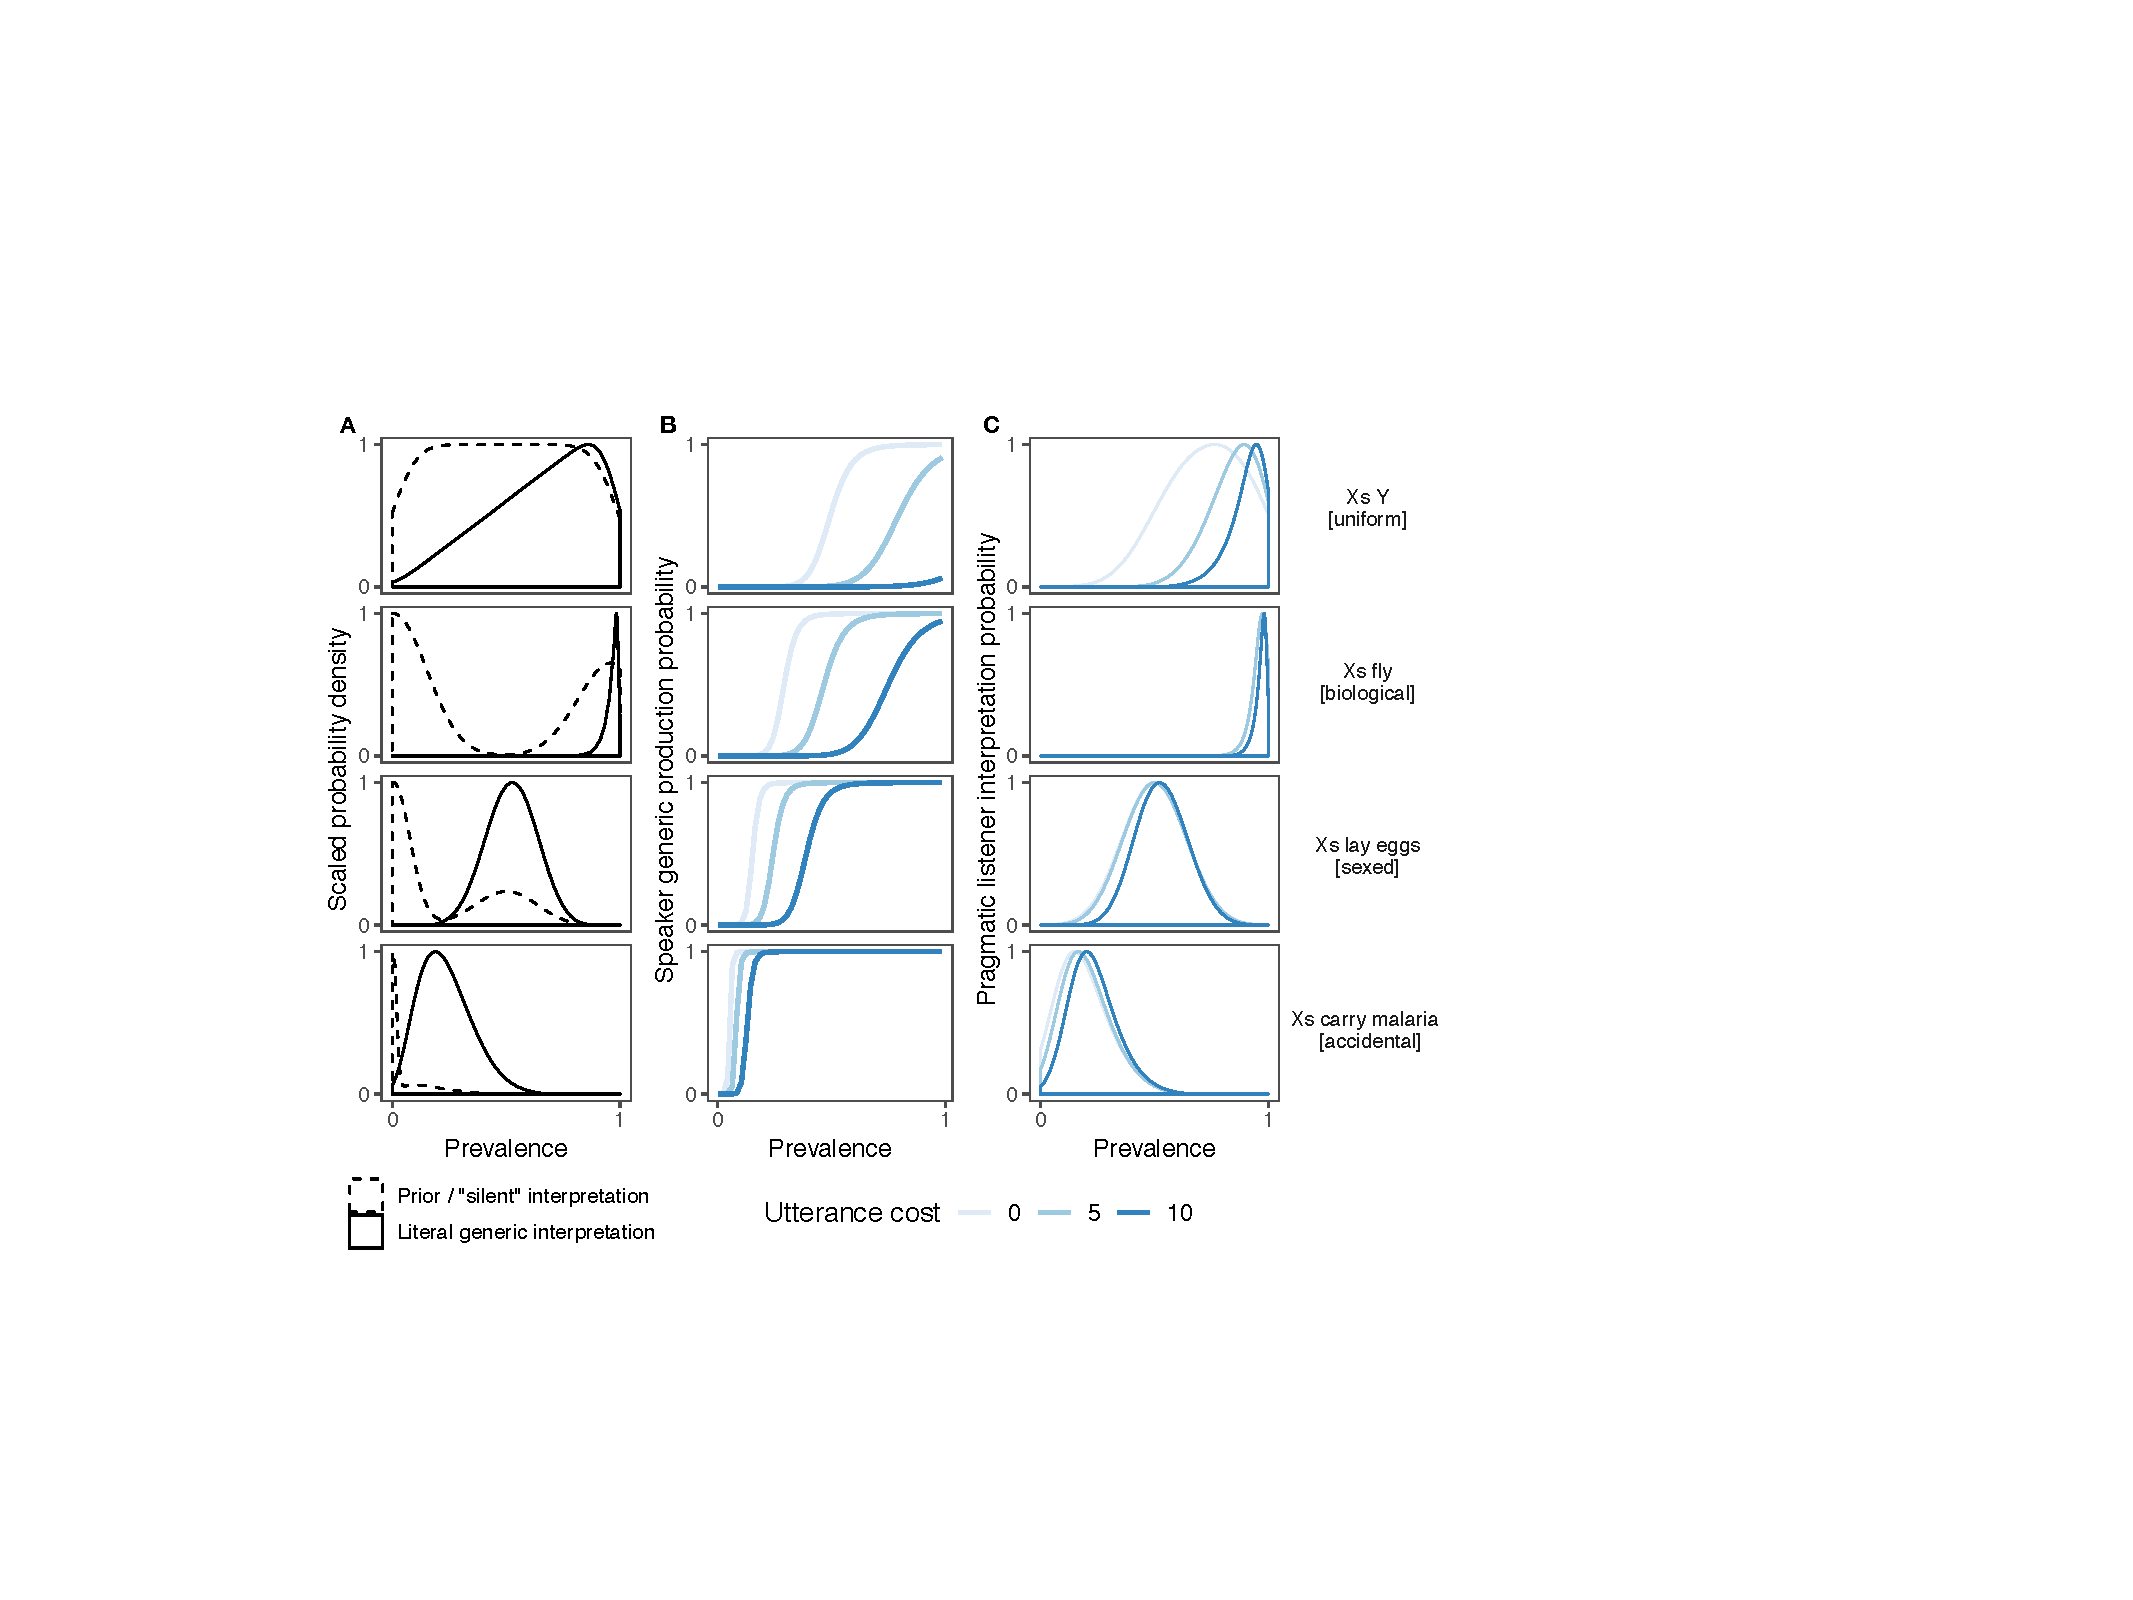
\includegraphics[width=0.8\textwidth]{figs/tripartite.pdf}
%\vspace{0.5cm}
%\caption{Examples of the three layers of the pragmatic interpretation model for four different properties. A: Literal listener $L_0$ interpretations (solid) for different prevalence priors (dashed). Priors also correspond to the literal interpretations of the ``silent'' utterance produced by the speaker $S_1$. B: Speaker $S_1$ production probabilities at different levels of prevalence for the generic utterance for three different costs of the generic utterance. C: Pragmatic listener interpretations of the generic utterance under different assumed costs of utterances. Differences between pragmatic and literal models are most pronounced for the priors with more uncertainty, such as the uniform prior. Speaker optimality parameter $\alpha$ set to 10 for panels B and C. Probability distributions are scaled so that the maximum density value in each panel is equal to 1. }
%\label{fig:tripartite}
%\end{figure}